\documentclass[12pt]{article}

\usepackage{amsmath}
\usepackage{amsfonts}
\usepackage{amssymb}
\usepackage{amsthm}
\usepackage{mathrsfs}

\usepackage[margin=2cm]{geometry}
\usepackage{graphicx}
\usepackage{xcolor}
\usepackage{enumitem}
\usepackage{hyperref}
\usepackage{tabularx}
\usepackage{float}

\usepackage{tikz}

% No indentation after new paragraph
\setlength{\parindent}{0cm}

% No vertical space above or below a math environment
\setlength{\abovedisplayskip}{0pt}
\setlength{\belowdisplayskip}{0pt}
\setlength{\abovedisplayshortskip}{0pt}
\setlength{\belowdisplayshortskip}{0pt} 

% Hyperlink setup
\hypersetup{
	colorlinks   = true,
	linkcolor=blue,
	citecolor=blue
}

% To use dottet line in table of contents
% https://tex.stackexchange.com/questions/53898/how-to-get-lines-with-dots-in-the-table-of-contents-for-sections
\usepackage{tocloft}

\newtheorem{theorem}{Theorem}[section]
\newtheorem{lemma}[theorem]{Lemma}
\newtheorem{proposition}[theorem]{Proposition}
\newtheorem{corollary}[theorem]{Corollary}
\newtheorem{definition}[theorem]{Definition}
\newtheorem{remark}[theorem]{Remark}
\newtheorem{example}[theorem]{Example}

% The basic number types N, Z, Q, R, C
\newcommand{\NN}{\mathbb{N}}
\newcommand{\ZZ}{\mathbb{Z}}
\newcommand{\QQ}{\mathbb{R}}
\newcommand{\RR}{\mathbb{R}}
\newcommand{\eRR}{(\minus\infty,\plus\infty]}
\newcommand{\CC}{\mathbb{C}}

% The fancy letters
\newcommand{\rH}{\mathcal{H}}
\newcommand{\rP}{\mathcal{P}}
\newcommand{\rD}{\mathscr{D}}
\newcommand{\rC}{\mathcal{C}}
\newcommand{\rX}{\mathcal{X}}
\newcommand{\rY}{\mathcal{Y}}
\newcommand{\rL}{\mathcal{L}}
\newcommand{\rK}{\mathcal{K}}

% Machine Learning
\newcommand{\trSet}{D_{\mathrm{Train}}}
\newcommand{\teSet}{D_{\mathrm{Test}}}
\newcommand{\daSet}{D}
\newcommand{\hyp}{\mathcal{F}}
\newcommand{\reMe}{\mu}
\newcommand{\emMe}{\mu_{\mathrm{emp}}}

% Common shortcuts
\newcommand{\ra}{\rightarrow}
\newcommand{\se}{\searrow}
\newcommand{\ane}{\nearrow}
\newcommand{\Ra}{\Rightarrow}
\newcommand{\sep}{\;\vert\;} % separator
\newcommand{\st}{\;:\;} % such that
\newcommand{\ha}{\rightharpoonup} % half arrow
\newcommand{\prt}{\partial}
\newcommand{\vp}{\varphi}

%Small plus and minus
\newcommand{\plus}{\raisebox{.2\height}{\scalebox{.8}{+}}}
\newcommand{\minus}{\raisebox{.2\height}{\scalebox{1}{-}}}
\newcommand{\sgeq}{\raisebox{.0\height}{\scalebox{.55}{$\geq$}}}

% Mathematical definitions
\newcommand{\atinner}[3]{\left\langle #1,\,#2\right\rangle_{#3}}
\newcommand{\inner}[2]{\atinner{#1}{#2}{\rH}}
\newcommand{\ltwoinner}[2]{\atinner{#1}{#2}{\ltwosub}}
\newcommand{\atnorm}[2]{\left\Vert #1\right\Vert_{#2}}
\newcommand{\abs}[1]{\left\vert #1\right\vert}
\newcommand{\norm}[1]{\atnorm{#1}{\rH}}
\newcommand{\infnorm}[1]{\atnorm{#1}{\infty}}
\newcommand{\normltwoat}[2]{\Vert #1\Vert_{L^2(#2;\rH)}}
\newcommand{\normltwo}[1]{\normltwoat{#1}{0,T}}
\newcommand{\normloneat}[2]{\Vert #1\Vert_{L^1(#2;\,\rH)}}
\newcommand{\normlone}[1]{\normloneat{#1}{0,T}}
\newcommand{\norminf}[1]{\atnorm{#1}{\infty}}
\newcommand{\simplies}{\;\;\Rightarrow\;\;}
\newcommand{\qimplies}{\qquad\Rightarrow\qquad}
\newcommand{\sequiv}{\;\;\Leftrightarrow\;\;}
\newcommand{\qequiv}{\qquad\Leftrightarrow\qquad}
\DeclareMathOperator{\idm}{\mathrm{id}}
\DeclareMathOperator{\conv}{\mathrm{conv}\,}
\DeclareMathOperator{\cl}{\mathrm{cl}\,}
\DeclareMathOperator{\supp}{\mathrm{supp}}
\newcommand{\id}{\idm_{\rH}}
\newcommand{\idltwo}{\idm_{\ltwosub}}
\DeclareMathOperator{\res}{\mathcal{J}}
\DeclareMathOperator{\pr}{\mathrm{Pr}}
\DeclareMathOperator{\dist}{\mathrm{dist}}
\DeclareMathOperator{\esssup}{\mathrm{ess}\,\sup}
\DeclareMathOperator{\ltwomap}{\mathcal{I}}
\DeclareMathOperator*{\minimize}{\mathrm{minimize}}
\DeclareMathOperator*{\subj}{\mathrm{subject\;to}}
\DeclareMathOperator*{\Int}{\mathrm{int}}
\newcommand{\atlp}[3]{L^{#1}\big(#2;\,#3\big)}
\newcommand{\atlpsub}[3]{L^{#1}(#2;\,#3)}
\newcommand{\lpgeneral}[1]{\atlp{p}{#1}{\rH}}
\newcommand{\linf}{\atlp{\infty}{0,T}{\rH}}
\newcommand{\linfnn}{\atlp{\infty}{0,\plus\infty}{\rH}}
\newcommand{\lone}{\atlp{1}{0,T}{\rH}}
\newcommand{\ltwo}{\atlp{2}{0,T}{\rH}}
\newcommand{\ltwosub}{L^2}
\newcommand{\wonetwo}{W^{1,2}(0,T;\,\rH)}
\newcommand{\woneone}{W^{1,1}(0,T;\,\rH)}
\newcommand{\atcts}[2]{C^{\, 0}\big(#1;\,#2\big)}
\newcommand{\cts}{\atcts{0,T}{\rH}}
\newcommand{\bv}{\mathrm{BV}(0,T;\,\rH)}

\begin{document}
	\begin{titlepage}
	\begin{center}
		\vspace*{1cm}
		
		\large
		\textbf{Jethro Warnett}
		
		\vspace{1.5cm}
		
		\Huge{\textbf{Gradient Flows in Hilbert Spaces with Application}}
		
		\vfill
		
		\large
		\textit{Semester Paper supervised by:} Prof. Dr. Alessio Figalli
		
		\vspace{0.8cm}
		
		ETH Zürich, Herbstsemester 2021
	\end{center}
\end{titlepage}
	\section{Abstract}
The paper presents a collage of results for the theory of gradient flow
from the textbook \cite{brezis1973ope} from Haïm Brézis.
The main focus is placed on maximal monotone multivalued
operators in $ \RR $-Hilbert spaces and on the
inhomogeneous generalised gradient descent evolution
equation. In particular we study the case of when
the maximal monotone multivalued operator is the sub differential
operator of a proper convex lower semi continuous function 
on a $ \RR $-Hilbert space.
The paper demonstrates at the end how the theory of gradient flow
is applied in machine learning with an example
in ridge regression. 
	
	\renewcommand{\cftsecleader}{\cftdotfill{\cftdotsep}}	
	\begingroup
	\let\clearpage\relax
	\tableofcontents
	
	\section{Introduction}
The implementation and use of machine learning algorithms to solve
intricate and complex problems in areas such as data analysis
has been staggering in recent years. 
This is not surprising due to the ability of the state-of-the-art
machine learning algorithms to efficiently and reliably solve
problems, which are impracticable if not infeasible
for a human to attempt to resolve. These problems include
semantic segmentation \cite{DBLP:journals/corr/BadrinarayananK15},
language translation \cite{edunov2018understanding}
or speech recognition \cite{park2020improved}. 
The fundamental algorithm that is used in machine learning (or at least a variant) is called the discrete gradient descent method.
The theory behind this algorithm finds some of its origin 
from the theory of maximal monotone multivalued operators 
from Haïm Brezis \cite{brezis1973ope}.
For a detailed account of the history behind the theory
of maximal monotone multivalued operators, we
refer interested readers to the paper \cite{borwein2010fifty}.\medskip

This semester paper presents the theory of
maximal monotone operators and in particular
the theory of gradient flow
from the textbook \cite{brezis1973ope} from Haïm Brézis
and indicates the connection to machine learning algorithms.\medskip

\subsection{Semester Paper Structure}
In Section 3 we state the theory of maximal monotone multivalued
operators in $ \RR $-Hilbert spaces and study
in particular the subdifferential operator of 
proper convex lower semicontinuous maps.\smallskip

We start section 4 by introducing the reader to
some preliminaries of function spaces over
a $ \RR $-Hilbert space. We proceed by
introducing the evolution equation
of the generalised gradient descent equation,
which is defined by
\begin{align*}
	\begin{cases}
		\partial_t u+Au \ni f & \text{ on }[0,T],\\
		u=u_0 & \text{ on }\{0\}.
	\end{cases}
\end{align*}
First we consider the homogeneous case where $ f=0 $,
and then the inhomogeneous case with 
$ f\in\lone $. We finish the section by investigating the special case, 
where the maximal multivalued operator $ A $
is the subdifferential of a proper
convex lower semi continuous function.\smallskip 

In Section 5 we provide a brief explanation of what neural networks
are in machine learning and how gradient flow is applied in
algorithms to train these networks. We finish the section by
presenting an example in ridge regression 
as described in originally in the paper \cite{hoerl1970ridge}, 
or for a more recent version in \cite{signoretto2014learning}.
Alongside this example we conduct and present the results
of a numerical experiment of ridge regression.\medskip

All the material that was used to write this semester
paper can be found on the following public repository
on
\href{https://github.com/JethroWarnettMath/Semester-Project-Gradient-Flow-HS2021}
{GitHub}.\medskip

Throughout the entire paper we assume that $ \rH $ is a $ \RR $-Hilbert space. 
We denote by $ \inner{\cdot}{\cdot} $ the inner product of $ \rH $, 
and by $ \norm{\cdot} $ the induced norm of $ \rH $, i.e. $ \norm{x}=\sqrt{\inner{x}{x}} $
for all $ x\in\rH $.
	\section{Maximal Monotone Operators in Real Hilbert Spaces}

\subsection{Multivalued Operators}

In this section we will introduce a class of multivalued operators
in $\RR$-Hilbert spaces called maximal monotone operators and study
some of their properties. The theory of gradient flows is based on the class 
of these operators. We proof a criterion for these operators to be 
maximally monotone and use this condition to present a few examples.

\begin{definition}
	A multivalued operator $ A $ in $ \rH $ is a mapping $ A:\rH \ra \rP(\rH)$,
	where $ \rP $ denotes the powerset. 
	The domain of $ A $ is defined by the set $ D(A):=\{x\in \rH \sep A(x) \neq \emptyset\} $ and the range of $ A $ is defined by 
	$ R(A):=\{y\in\rH \sep \exists x \in \rH \st y \in A(x) \} $.
	The mapping $ A $ is single valued, if all elements in the domain of $ A $
	are mapped to singletons.
\end{definition}

Throughout this paper we will make the following simplifications:
For any $ x \in \rH $ we write $ Ax $ as short hand for $ A(x) $, and 
we identify single valued operators with self-mappings in $ \rH $,
i.e. functions of the form $ \rH\ra\rH $. 
We assume $ A\eta $ is any value $ \xi\in A\eta $ for $ \eta\in D(A) $ 
unless specified otherwise. \medskip

It is useful to relate multivalued operator with their graphs in $ \rH\times \rH $. 
This is because set inclusion will endow the set of multivalued operators in 
$ \rH $ with a partial order.

\begin{definition}
	Let $ A $ be a multivalued operator in $ \rH $.
	The graph of $ A $ is defined by the set 
	$ \{(\eta,\xi) \sep \eta\in D(A),\; \xi\in A\eta\} $.
	We identify the multivalued operator $ A $ with its own graph. 
\end{definition}

We need multivalued operators to be compatible with the vector space structure of 
$ \rH $. This motivates the following definition.

\begin{definition}
	Let $ A $ and $ B $ be multivalued operators in $ \rH $ and $ \lambda \in \RR$ any real value. We construct the following multivalued operators in $ \rH $:
	\begin{itemize}
		\item The sum $ A+B $ is defined by $ (A+B)x:=\{y+z \sep y \in Ax,\; z \in Bx\} $ for all $ x\in\rH $, with the domain given by the intersection $ D(A)\cap D(B) $.
		\item The scalar multiple $ \lambda A $ is defined by 
		$ \lambda Ax:=\{\lambda y \sep y \in Ax\} $ for all $ x\in\rH $, 
		whose domain coincides with that of $ A $.
		\item The inverse $ A^{-1} $ of $ A $ is defined by its graph 
		$ A^{-1}:=\{(y,x) \sep (x,y) \in A\} $. The domain and range of $ A^{-1} $ 
		coincide with the ones from $ A $ but interchanged, 
		this means we have that $ D(A^{-1}) = R(A) $ and $ R(A^{-1}) = D(A) $.
	\end{itemize}
\end{definition}

In the Hilbert space $ \RR $ a mapping $ f:\RR\ra\RR $ is monotonically 
increasing if and only if 
it satisfies for the following inequality
\begin{align*}
	\big(f(x)-f(y)\big)\cdot \big(x-y\big)\geq 0
	\qquad \forall x,y\in\RR.
\end{align*} 
This notion of monotonicity can be generalised to any $ \RR $-Hilbert space.

\begin{definition}
	We say a multivalued operator $ A $ in $ \rH $ is monotone, 
	if it fulfils the following inequality
	\begin{align*}
		\inner{\xi_1-\xi_2}{\eta_1-\eta_2}\geq 0
		\qquad \forall (\eta_1,\xi_1),(\eta_2,\xi_2)\in A.
	\end{align*}
\end{definition}

\begin{lemma}\label{lemma:char of mon op}
	Let $ A $ be a multivalued operator in $ \rH $.
	Then $ A $ is monotone if and only if
	for all $ \lambda>0 $ the following inequality holds true
	\begin{align}\label{equation:char of mon op}
		\norm{\eta_1-\eta_1}\leq 
		\norm{(\id+\lambda A)\eta_1-(\id+\lambda A)\eta_2}
		\qquad\forall \eta_1,\eta_2\in D(A).
	\end{align}
\end{lemma}
\begin{proof}
	First suppose the inequality \eqref{equation:char of mon op} 
	holds true. Thus by squaring and restructuring the equations
	we get the equivalent statement
	\begin{align*}
		-\lambda^2 \norm{A\eta_1-A\eta_2}^2\leq 2\lambda 
		\inner{A\eta_1-A\eta_2}{\eta_1-\eta_2},
	\end{align*}
	If we divide by $ \lambda $ and take the limit $ \lambda\se 0 $,
	we get that $ A $ is monotone. On the other hand, if $ A $ is
	monotone, we can reverse the arguments to see that the inequality
	\eqref{equation:char of mon op} is correct.
\end{proof}

\begin{remark}
	Lemma \ref{lemma:char of mon op} shows how the notion of a monotone
	multivalued operator can be extended to include Banach spaces. This
	generalization is investigated in papers such as \cite{10.2307/2373376}. 
\end{remark}

Of particular interest are the maximal elements in the set of monotone 
multivalued operators in $ \rH $ that are partially ordered by the set inclusions
of their graphs.

\begin{definition}
	A monotone multivalued operator $ A $ in $ \rH $ is maximally monotone, if its graph is 
	inclusion-wise maximal in the set of graphs of monotone multivalued operators in $ \rH $. 
	This means that if $ B $ is a monotone multivalued operator in $ \rH $
	with $ A\subseteq B $, then $ A=B $. 
\end{definition}

\begin{remark}\label{remark:char graph el}
	The graph of a maximally monotone operator $ A $ has an equivalent
	definition, on which this semester project will rely on many times. Namely for 
	$ (x,y)\in\rH \times \rH $ we have
	\begin{align}\label{eq1:remark:char graph el}
		(x,y)\in A
		\qequiv
		\inner{y-\xi}{x-\eta}\geq 0
		\qquad\forall (\eta,\xi)\in A.
	\end{align} 
\end{remark}

With the condition \eqref{eq1:remark:char graph el} 
we can build other maximally monotone
operators from an existing one.

\begin{example}\label{example:easy examples of max mon op}
	If $ A $ is a maximally monotone operator on $ \rH $, then so to is
	the scalar multiple $ \lambda A $ for all $ \lambda>0 $ and the inverse
	$ A^{-1} $. \smallskip
	
	In general the same cannot be said about the finite sum of maximally 
	monotone multivalued operators in $ \rH $, as the intersection
	of their domains may be empty. Although there are conditions on the domain
	that permit the aforementioned sum to be maximally monotone 
	(cf. \cite[Chapter 2.6]{brezis1973ope}).
\end{example}

A maximally monotone multivalued operator imposes structural constraints 
on the image of individual elements.

\begin{lemma}\label{lemma:mapped element is weak cl and conv}
	Let $ A $ be a maximally monotone operator in $ \rH $  and
	$ \eta\in D(A) $. Then the set $ A\eta $ is convex and weakly closed 
	for all $ \eta \in D(A) $. In addition for any
	$ \eta_1,\eta_2\in D(A) $ we have
	that $ \Int A\eta_1\cap \Int A\eta_2=\emptyset $, whenever $ \eta_1\neq \eta_2 $.
\end{lemma}
\begin{proof}
	"$ A\eta $ is convex": For all  $ \theta\in[0,1] $ and $ \xi_1,\xi_2\in A\eta $
	we have $ \theta\xi_1+(1-\theta)\xi_2\in A\eta $, since the value satisfies
	the condition \eqref{eq1:remark:char graph el} by the following computation
	\begin{align*}
		\begin{split}
			\inner{\theta \xi_1 + (1-\theta) \xi_2 -y}{\eta-x}
			&=\inner{\theta (\xi_1-y) + (1-\theta) (\xi_2 -y) }{\eta-x}\\
			&=\theta\inner{\xi_1-y}{\eta-x}
			+(1-\theta)\inner{\xi_2 -y}{\eta-x}\\
			& \geq 0
		\end{split}
		\qquad
		\forall (x,y)\in A.
	\end{align*}
	"$ A\eta $ is weakly closed": Let $ (\xi_n)_{n\in\NN}\subseteq A\eta$ 
	be any sequence such that $ \xi_n\ha \xi $ for some $ \xi\in\rH $. 
	Then $ \xi\in A\eta $, as the value satisfies the condition
	\eqref{eq1:remark:char graph el} by the following calculation
	\begin{align*}
		\inner{\xi-y}{\eta-x}
		=\lim_{n\ra\infty}\inner{\xi_n-y}{\eta-x}
		\geq 0
		\qquad
		\forall (x,y)\in A.
	\end{align*}
	"$\Int A\eta_1\cap \Int A\eta_2=\emptyset$": Suppose there exists
	$ \xi\in\rH $ and $ \varepsilon>0 $, such that every $ x\in\rH $ with
	$ \norm{x}<\varepsilon $ satisfies $ \xi+x\in A \eta_1\cap A\eta_2 $.
	Then as $ A $ is maximally monotone we see
	\begin{align*}
		\inner{x}{\eta_1-\eta_2}
		=\inner{(\xi+x)-\xi}{\eta_1-\eta_2}
		\geq 0.
	\end{align*}
	As this inequality must hold for all elements $ x $ in a neighbourhood
	of $ 0 $, we deduce that the identity $ \eta_1=\eta_2 $ must stand.
\end{proof}

We will see in Theorem \ref{theorem:res is proj in limit and dom is conv},
in combination with example \ref{example:easy examples of max mon op},
that a maximally monotone operator even imposes structural constraints 
on its domain and range.\smallskip

Next we present a criterion for a multivalued operator to be
maximally monotone. This proposition will require the use of the
following theorem, a proof of which can be found in 
\cite[Theorem 2.1]{brezis1973ope}.

\begin{theorem}\label{theorem:monotone extension}
	Let $ C $ be a closed convex set in $ \rH $ and $ A $ a monotone operator in $ \rH $.
	For all $ y \in \rH $ there exists $ x\in C $ such that
	\begin{align*}
		\inner{\xi + x}{\eta - x}\geq \inner{y}{\eta - x}
		\quad \forall (\eta,\xi) \in A.
	\end{align*}
\end{theorem}

This theorem lets us state a useful 
criteria for a multivalued operator to be maximally monotone.
In fact we will need these conditions for the examples at the end of this section.

\begin{proposition}\label{proposition:criteria for max mon}
	Let $ A $ be a multivalued operator in $ \rH $. Then the following
	are equivalent
	\begin{enumerate}[label=(\roman*)]
		\item $ A $ is maximally monotone.
		\item $ A $ is monotone and $ R(\id + A)=\rH $.
	\end{enumerate}
\end{proposition}
\begin{proof}
	"(i) $\Ra$ (ii)":  
	If we set $ C=\rH $ in theorem \ref{theorem:monotone extension}, 
	then for all $ y\in\rH $ there exists $ x\in\rH $ with
	\begin{align*}
		\inner{\xi + x}{\eta - x}\geq \inner{y}{\eta - x}
		\quad \forall (\eta,\xi) \in A.
	\end{align*}
	By condition \eqref{eq1:remark:char graph el} we have
	that $ y-x\in Ax $ and thus
	$ y\in R(\id+ A) $. This proves $ R(\id+A)=\rH $.\smallskip
	
	"(ii) $\Ra$ (i)": Let $ B $ be a monotone multivalued operator 
	on $ \rH $ such that $ A\subseteq B $. By assumption for all 
	$ (\eta,\xi)\in B $ 
	there must exist $ z\in D(A) $ satisfying 
	$ \eta+\xi\in z+Az \subseteq z+Bz $. Clearly we have 
	$ \eta+\xi\in \eta+B\eta $.
	Then by using the monotonicity of $ B $, we compute
	\begin{align*}
		0\leq \inner{(\eta+\xi-z)-(\eta+\xi-\eta)}{z-\eta}=-\norm{\eta-z}^2\leq 0.
	\end{align*}
	This shows $ \eta = z $ and thus $ (\eta,\xi)\in A $. Then 
	$ A $ is maximally monotone as $ A=B $.\smallskip
\end{proof}

Of independent interest is that any multivalued monotone 
operator in $ \rH $ can be extended
to a maximally monotone operator. The extension of the domain 
can be restricted to at most the closure of the convex hull 
of the monotone operator.

\begin{corollary}\label{corollary:max mon ext}
	Let $ A $ be a monotone multivalued operator in $ \rH $. 
	There exists some maximally
	monotone operator $ B $ in $ \rH $ with $ A\subseteq B $ 
	and $ D(B)\subseteq \overline{\conv D(A)}$.
\end{corollary}
\begin{proof}
	Let us define the set $ \rD $ of all monotone multivalued
	operators $ B $ in $ \rH $ with $ A\subseteq B $ 
	and $ D(B)\subseteq \overline{\conv D(A)}$. The
	set is endowed with the partial order of the graphs of 
	multivalued operators in $ \rH $. The set $ \rD $
	is non-empty as it contains $ A $. Thus by
	Zorn's Lemma, there exists a maximal element $ B$ in $\rD $.\smallskip
	
	We claim that $ B $ is maximally monotone. Indeed 
	if we set $ C=\overline{\conv D(A)} $ in theorem 
	\ref{theorem:monotone extension}, 
	then for all $ y\in\rH $ there exists $ x\in C $ with
	\begin{align*}
		\inner{\xi + x}{\eta - x}\geq \inner{y}{\eta - x}
		\quad \forall (\eta,\xi) \in B.
	\end{align*}
	As $ B $ is maximal in $ \rD $, we have
	that $ y-x\in Bx $ and thus
	$ y\in R(\id+ B) $. From this we deduce $ R(\id+B)=\rH $.
	So by proposition \ref{proposition:criteria for max mon}
	we have that $ B $ is maximally monotone.
\end{proof}

\begin{remark}
	One may wonder if in corollary \ref{corollary:max mon ext},
	the domain of $ B $ can be restricted to a smaller
	set than $ \overline{\conv D(A)} $. We will see in
	theorem \ref{theorem:res is proj in limit and dom is conv}
	that this is not true.
\end{remark}

With proposition \ref{proposition:criteria for max mon} it is possible
to count some examples of maximally monotone operators.

\begin{example}\label{exampel:mon R funct op}
	Let $ f:\RR \ra \RR$ be a non-decreasing mapping. Define 
	the multivalued operator $ A $ in $ \RR $ by 
	$ A\eta:=[f(\eta-),f(\eta+)] $ for all $ \eta\in \RR $,
	with $ f(\eta\pm):=\lim_{h\se 0}f(\eta\pm h) $. Clearly
	$ R(A) $ is a closed interval in $ \RR $ and thus 
	$ \idm_{\RR}+A $ is a surjective multivalued operator
	and it is monotone as $ f $ is non-decreasing.
	Thus by proposition \ref{proposition:criteria for max mon}
	we know that $ A $ is maximally monotone.
\end{example}

\begin{example}\label{example:map max mon op from H to L2}
	There is a mapping 
	$ \ltwomap $ from maximally monotone
	operators in $ \rH $ into maximally monotone operators in the 
	$ \RR $-Hilbert space\footnote{See definition 
	\ref{definition:lp space in hilbert space}} $ \ltwo $.
	For any maximally monotone operator $ A $ in $ \rH $ we define
	the multivalued operator $ \ltwomap A $ by
	\begin{align*}
		\ltwomap Af=\{u\in\ltwo \sep u(t)\in Af(t)\text{ for a.e. }t\in [0,T]\}
		\qquad\forall f\in D(\ltwomap A),
	\end{align*}
	where the domain of $ \,\ltwomap A $ is defined by 
	$ \{f\in\ltwo\sep f(t)\in D(A)\text{ for a.e. }t\in [0,T] \}$. 
	To show that $ \ltwomap A $ is maximally monotone,
	by proposition \ref{proposition:criteria for max mon}
	it suffices to verify that $ \ltwomap A $
	is monotone and $ R(\idltwo+\ltwomap A)=\ltwo $.
	Then $ \ltwomap A $ is indeed monotone, since for all 
	$ (f_1, u_1),(f_2,u_2)\in\ltwomap A $ we see
	by the monotonicity of $ A $ that
	\begin{align*}
		\ltwoinner{u_1-u_2}{f_1-f_2}
		=\int_0^T
		\inner{u_1-u_2}{f_1-f_2}\,dt
		\geq 0.
	\end{align*}
	Moreover it holds that $ R(\idltwo+\ltwomap A)=\ltwo $,
	since for any
	$ u\in\ltwo $ there exists for almost all $ t\in[0,T] $
	some $ f(t)\in D(A) $ with $ u(t)=f(t)+Af(t) $.
	We have that $ f\in \ltwo $ since
	by lemma \ref{lemma:res is contr onto dom} we know that
	$ \norm{f(t)}\leq \norm{u(t)} $ for almost all $ t\in[0,T] $
	and thus by the dominated convergence theorem we infer the claim. 
	Furthermore $ f\in D(\ltwomap A) $ and
	$ u=f+\ltwomap A f $.
\end{example}

%% Interesting conseuqeunce
%\begin{remark}
%	If we apply the operator $ \ltwomap $ consecutively 
%	$ k $ times for $ k\geq 1 $, then \textbf{replace
%	$ \rH $ with $ \rH^k $} 
%	\begin{align*}
%		\left\{\begin{array}{l}
%			\ltwomap^k Af=
%			\{u\in\ltwo \sep u(t)\in Af(t)\text{ for a.e. }t\in [0,T]\}
%			\qquad\forall f\in D(\ltwomap A)\\
%			D(\ltwomap^k A)=
%			\{f\in\ltwo\sep f(t)\in D(A)\text{ for a.e. }t\in [0,T] \}
%		\end{array}
%		\right.
%	\end{align*}
%\end{remark}

\begin{example}\label{example:sem pos def lin op is max mon}
	Let $ A $ be a linear operator in $ \rH $. Then
	$ A $ is maximally monotone if and only if $ A $
	is positive semi-definite, the range of $ A $
	is dense in $ \rH $ and $ A $ is closed under
	monotone extensions. \smallskip
	
	By definition the linear operator $ A $ is
	positive semi-definite if and only if its
	monotone.\smallskip
	
	So suppose first that $ A $ is maximally monotone.
	To show that the range is dense, suppose that $ y\in R(A)^{\bot} $. 
	So $ \inner{A\eta-y}{\eta-0}\geq 0 $ for all 
	$ \eta\in D(A) $ and thus by condition 
	\eqref{eq1:remark:char graph el} we have $ y=A0=0 $.
	The fact that $ A $ is closed under monotone 
	extensions holds by definition.\smallskip
	
	For the converse direction, suppose that $ A $ has
	a dense range and is closed under monotone extensions. 
	Assume that the pair $ (x,y)\in \rH\times \rH $
	satisfies the necessary condition \eqref{eq1:remark:char graph el},
	that is $ \inner{A\eta-y}{\eta-x}\geq 0 $ for all $ \eta\in D(A) $. 
	Then the linear mapping $ D(A)+\RR x\rightarrow\rH, 
	\eta+\lambda x\mapsto A\eta+\lambda y$ is a monotonic
	extension of $ A $. Indeed for $ \eta_1,\eta_2\in D(A) $
	and $ \lambda_1,\lambda_2\in\RR $ we compute by the linearity
	of $ A $ and the property of $ (x,y) $ that
	\begin{align*}
		&\inner{(A\eta_1+\lambda_1 y)-(A\eta_2+\lambda_2 y)}{(\eta_1+\lambda_1 x)
		-(\eta_2-\lambda_2 x)}\\
		&\qquad\qquad\qquad
		=\inner{A(\eta_1-\eta_2)+(\lambda_1-\lambda_2)y}{
			(\eta_1-\eta_2)+(\lambda_1-\lambda_2)x}\\
		&\qquad\qquad\qquad\geq 0.
	\end{align*}
	As $ A $ is closed under monotonic extensions, we 
	determine that $ x\in D(A) $ and $ Ax=y $. Hence we see
	from condition \eqref{eq1:remark:char graph el} that
	$ A $ is a maximally monotone operator.
\end{example}

\begin{example}\label{example:spat der of W is max mon}
	Let $ \rK $ be any $ \RR $-Hilbert space and define 
	the $ \RR $-Hilbert space $ \rH=L^2(0,\rL;\,\rK) $ 
	and the linear operator $ A $ on $ \rH $ as the spatial 
	derivative $ A=\prt_x $ with domain
	defined by the set\footnote{The set $ W^{1,p}(0,\rL; \rK) $
		is the Sobolev space 
		(cf. definition \ref{definition:sobolev space for hilbert space})}
	$ \{f\in W^{1,2}(0,\rL; \rK)\sep f(0)=0\} $. 
	The operator is positive semi-definite since
	\begin{align*}
		\ltwoinner{Af}{f}
		=\int_0^\rL\atinner{\prt_x f}{f}{\rK}\,dx
		=\frac{1}{2}\atnorm{f(\rL)}{\rK}^2
		\geq 0.
	\end{align*}
	It can be shown that $ A $ has dense range in $ \rH $.
	Indeed if $ g\in\rH $ is such that $ g(0)=0 $,
	then its integral $ G(x):=\int_0^x g(y)\,dy $
	for $ x\in[0,T] $ is in the domain of $ A $
	and it will map to $ g $, i.e. $ AG=g $.
	It thus suffices to prove that any constant function
	can be approximated arbitrarily well. But this is clear, by
	taking the integral of a step function that is sufficiently 
	large near a neighbourhood of $ 0 $ and vanishes everywhere else.
	Thus by example \ref{example:sem pos def lin op is max mon}
	we know that $ A $ is maximally monotone.\smallskip
	
	In fact for any $ u_0\in \rK $ we know that $ A+u_0 $ is
	also maximally monotone. Thus we may exchange the domain of
	$ A $ with the domain that sets $ u_0 $ as an initial 
	condition, i.e. we can swap $ D(A) $
	with the set $\{f\in W^{1,2}(0,\rL;\rK)\sep f(0)=u_0\} $.
\end{example}

\subsection{The Resolvent and Yosida Approximation}

In this section we will define two single valued operators, namely
the resolvent and the Yosida approximation of maximal monotone operators.
These constructions are very important tools for the
study of maximal monotone operators and gradient flow, on
which this paper will rely on many times. In addition we will
show for a maximal monotone multivalued operator,
that the closure of its domain is convex and that its
resolvent strongly converges to the projection operator of its own domain.
We end the section by studying the attributes of 
the Yosida approximation.\smallskip

Throughout this section let $ A $ be a maximally monotone multivalued
operator in $ \rH $. For a convex set $ C\subseteq \rH $, we
let $ \pr_C:\rH\ra \overline{C} $ be the projection mapping
of $ \rH $ onto the closure of $ C $.\smallskip

\begin{definition}\label{def:resolvent}
	Let $ A $ be a maximally monotone multivalued operator and $ \lambda > 0 $ arbitrary. Define the resolvent of $ A $ (with parameter $ \lambda $) as
	the multivalued operator $ \res_\lambda:=(\id+\lambda A)^{-1} $.
\end{definition}

\begin{lemma}\label{lemma:res is contr onto dom}
	The resolvent $ \res_\lambda $ of a maximally monotone multivalued operator 
	$ A $ in $ \rH $ is a single valued operator with image $ D(A) $. 
	Specifically it is a contraction from $ \rH $ onto $ D(A) $.
\end{lemma}
\begin{proof}
	From proposition \ref{proposition:criteria for max mon} we learn
	that $ D(\res_\lambda)=\rH $. By definition of the inverse operator, 
	we have that $ R(\res_\lambda)=D(A) $.
	From lemma \ref{lemma:char of mon op} we learn the resolvent is a contraction. 
	In particular this means that the mapping is single valued.
\end{proof}

We analyze the asymptotic behavior of the resolvent $ \res_\lambda $
of $ A $ whenever $ \lambda\se 0 $. 

\begin{example}
	Let $ A $ be defined as in example \ref{exampel:mon R funct op} with 
	$ f:(-1,1)\rightarrow \RR;\, x \ra \ln(1-x)-\ln(1+x) $. From
	example \ref{exampel:mon R funct op} we know that 
	$ A $ is a maximally monotone operator with $ D(A)=(-1,1) $. 
	Note for all $ x\in (-1,1) $ we have $ x+\lambda Ax
	= x +\lambda f(x) \ra x $ when $ \lambda \se 0 $. This
	shows that $ \res_\lambda x \ra \pr_{D(A)} x $ 
	for all $ x\in\RR $. Compare this with figure 
	\ref{fig:example of projection}.
\end{example}

\begin{example}\label{example:res of spat der of W}
	Define the Hilbert space $ \rH $ and maximally monotone
	multivalued operator $ A $
	as in example \ref{example:spat der of W is max mon}.
	We assume that $ D(A) $ sets $ u_0\in\rH $ as an initial condition
	for any $ u_0\in\rH $. Thus for every $ u\in D(A) $ and all $ \lambda >0 $
	the resolvent $ \res_\lambda $ of $ A $ has the explicit form
	\begin{align*}
		\res_\lambda u(x)
		=e^{-\frac{x}{\lambda}}u_0
		+\frac{1}{\lambda}\int_0^x e^{\frac{y-x}{\lambda}} u(y)\,dy
		\qquad\forall x\in[0,\rL].
	\end{align*}
	Indeed the following computation verifies the claim
	\begin{align*}
		\begin{split}
			(\idltwo+\lambda A)&
			e^{-\frac{x}{\lambda}}u_0
			+\frac{1}{\lambda}\int_0^x e^{\frac{y-x}{\lambda}} u(y)\,dy\\
			&=e^{-\frac{x}{\lambda}}u_0
			+\lambda A e^{-\frac{x}{\lambda}}u_0
			+\frac{1}{\lambda}e^{\frac{-x}{\lambda}}
			\int_0^x e^{\frac{y}{\lambda}} u(y)\,dy
			+A e^{\frac{-x}{\lambda}}\int_0^x e^{\frac{y}{\lambda}} u(y)\,dy\\
			&=e^{-\frac{x}{\lambda}}u_0
			-e^{\frac{-x}{\lambda}} u_0
			+\frac{1}{\lambda}e^{\frac{-x}{\lambda}}
			\int_0^x e^{\frac{y}{\lambda}} u(y)\,dy
			-\frac{1}{\lambda}e^{\frac{-x}{\lambda}}
			\int_0^x e^{\frac{-x}{\lambda}}u(y)\,dy
			+u(x)\\
			&=u(x).
		\end{split}
		\qquad\forall x\in[0,\rL].
	\end{align*}
	Using integration by
	parts and the weak derivative\footnote{See 
		definition \ref{definition:weak der}},
	we see that $ \res_\lambda\ra\idltwo $ whenever $ \lambda\se 0 $.
	\begin{align*}
		\res_\lambda u(x)
		=e^{-\frac{x}{\lambda}}u_0
		+\frac{1}{\lambda}\int_0^x e^{\frac{y-x}{\lambda}} u(y)\,dy
		=e^{-\frac{x}{\lambda}}u_0
		+\left[e^{\frac{y-x}{\lambda}} u(y)\right]_0^x
		-\int_0^x e^{\frac{y-x}{\lambda}} \prt_y u(y)\,dy.
	\end{align*}
	If we take the limit $ \lambda\ra 0 $ we see that
	\begin{align*}
		\lim_{\lambda\se 0}\res_\lambda u(x)
		=\lim_{\lambda\se 0} e^{-\frac{x}{\lambda}}u_0
		+\left[e^{\frac{y-x}{\lambda}} u(y)\right]_0^x
		-\int_0^x e^{\frac{y-x}{\lambda}} \prt_y u(y)\,dy
		=u(x).
	\end{align*}
\end{example}

\begin{figure}
	\centering
	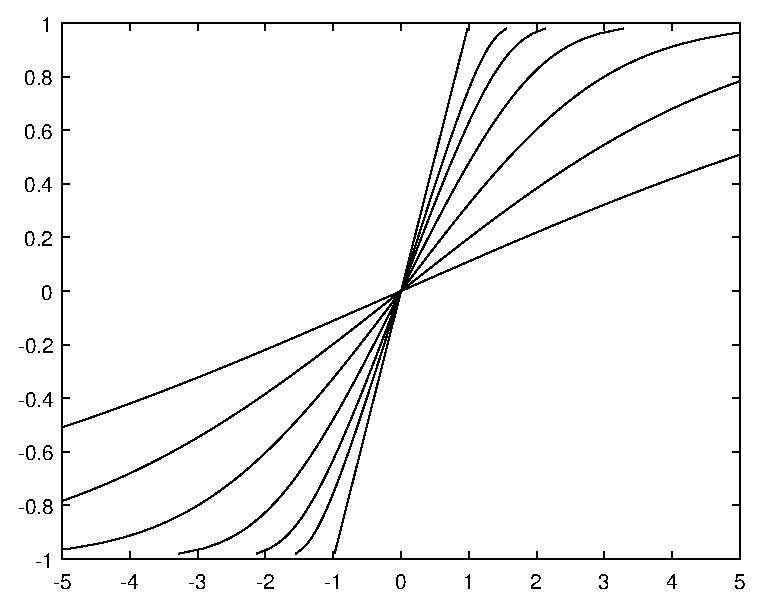
\includegraphics{projectionExample}
	\caption{Shows how the resolvent $ \res_\lambda $
		approximates the projection $ \pr_{D(A)} $ whenever
		$ \lambda\se 0 $.}
	\label{fig:example of projection}
\end{figure}

The following theorem shows that the examples generalise to all maximal monotone
operators.

\begin{theorem}\label{theorem:res is proj in limit and dom is conv}
	The set $ \overline{D(A)} $ is convex and 
	$ \res_\lambda x \ra \pr_{\overline{D(A)}} x $ 
	as $ \lambda\se 0 $ for all $ x\in\rH $.
\end{theorem}
\begin{proof}
	Define $ C:=\overline{\conv D(A)}  $ and for any $ x\in\rH $
	define $ x_\lambda:=\res_\lambda x $. First we show
	that $ x_\lambda $ is bounded as $ \lambda \se 0 $. 
	By definition of the resolvent 
	we have $ x\in x_\lambda+\lambda A x_\lambda $,
	then with the monotonicity of $ A $ we get
	for any $ (\eta,\xi)\in A $ the inequality
	\begin{align*}
		\inner{\frac{x-x_\lambda}{\lambda}-\xi}{x_\lambda-\eta}\geq 0.
	\end{align*}
	We multiply with $ \lambda $ and use the Cauchy-Schwartz inequality 
	to prove the boundedness of $ x_\lambda $ by
	\begin{align}\label{eq1:theorem:res is proj in limit and dom is conv}
		\norm{x_\lambda}^2
		\leq \inner{\lambda \xi - x}{\eta}+\inner{x_\lambda}{\eta+x-\lambda \xi}
		\leq \inner{\lambda \xi - x}{\eta}+\norm{x_\lambda}\norm{\eta+x-\lambda \xi}.
	\end{align}
	Next we show that $ x_\lambda \ra \pr_{\overline{D(A)}} x $ 
	as $ \lambda\se 0 $. 
	By lemma \ref{lemma:res is contr onto dom} we know that
	$ (x_\lambda)_{\lambda>0} $ is contained in $ D(A) $.
	As any bounded sequence in a Hilbert space has a weakly convergent
	subsequence,
	there exists a positive null-sequence $ (\lambda_n)_{n\in\NN} $ such
	that $ x_{\lambda_n} \ha x_0$ for some $ x_0 \in C $. If we apply the
	limit to \eqref{eq1:theorem:res is proj in limit and dom is conv}, 
	we get
	\begin{align}\label{eq2:theorem:res is proj in limit and dom is conv}
		\norm{x_0}^2
		\leq \limsup_{n \ra \infty}\norm{x_\lambda}^2
		=\inner{x_0}{\eta+x}-\inner{x}{\eta}
		\qimplies
		\inner{x-x_0}{\eta-x_0}
		\leq 0.
	\end{align}
	Observe the inequality on the right hand side in 
	\eqref{eq2:theorem:res is proj in limit and dom is conv}
	holds for all $ \eta \in D(A) $ and thus for all $ \eta \in C $
	(by a similar argument as in remark 
	\ref{lemma:mapped element is weak cl and conv}).
	Yet as $ C $ is closed and convex, this inequality 
	can only hold if $ x_0=\pr_{C}x $. Note that this result is independent of 
	the choice of null-sequence, which implies $ x_\lambda \ha \pr_{C}x $
	as $ \lambda \se 0 $.
	
	Lastly we must show that $ \overline{D(A)} $ is convex. 
	The same argument as above shows that the inequality on the 
	left hand side of \eqref{eq2:theorem:res is proj in limit and dom is conv}
	holds for all $ \eta\in C $. In particular if we set $ \eta=x_0 $
	in this inequality we deduce
	\begin{align}\label{eq3:theorem:res is proj in limit and dom is conv}
		\limsup_{\lambda \ra \infty}\norm{x_\lambda}^2
		= \inner{x_0}{x_0+x}-\inner{x}{x_0}
		= \norm{x_0}^2
	\end{align}
	Then \eqref{eq3:theorem:res is proj in limit and dom is conv}
	 and weak convergence is enough to imply $ x_\lambda \ra x_0 $.
	 Thus if $ x$ is in $ C $, then the sequence $ (x_\lambda)_{\lambda>0} $
	 is in $ D(A) $ and converges to $ x $. This implies $ \overline{D(A)}=C $
	 and hence $ \overline{D(A)} $ is convex.
\end{proof}

Now we introduce the Yosida approximation. A vital tool for
studying gradient flow and proper convex lower semi-continuous functions.

\begin{definition}\label{definition:Yosida Approximation}
	Let $ B $ be a maximally monotone multivalued operator in $ \rH $. 
	Define the Yosida approximation of $ B $ as the multivalued operator 
	$ B_\lambda:=\lambda^{-1}(\id-\res_\lambda) $.
\end{definition}

\begin{remark}\label{remark:triv prop yos app}
	$ \bullet $ The Yosida Approximation is a single valued operator on $ \rH $.
	\medskip
	
	$ \bullet $ The operators $ A $ and $ A_\lambda $ are 
	related for all $ x\in \rH $ by 
	$ A_\lambda x \in A \res_\lambda x $. Indeed 
	this follows from
	\begin{align*}
		A_\lambda x\in A\res_\lambda x
		\qequiv
		x\in (\id+\lambda A)\res_\lambda x 
		\qequiv
		x\in \res_\lambda^{-1}\res_\lambda x.
	\end{align*}
	
	$ \bullet $ In case $ A $ is a linear operator, then  
	$ A $ and $ A_\lambda $ are related for all 
	$ \eta\in D(A) $ by $ A_\lambda \eta=\res_\lambda A\eta $.
	The same argument as above holds, but we can replace the membership
	with an equality.
\end{remark}

\begin{definition}
	Let $ B $ be a maximally monotone multivalued operator in $ \rH $. Define the 
	minimum norm section $ B_0 $ of $ B $ to be the single valued operator with
	domain $ D(B_0)=D(B) $ and is defined by
	$ B_0 \eta := \arg\,\min_{x\in B\eta}\norm{x} $ for $ \eta\in D(B_0) $.
	This map is well-defined by lemma 
	\ref{lemma:mapped element is weak cl and conv}.
\end{definition}

We will need the following lemma a few times during this paper.

\begin{lemma}\label{lemma:weak seq cond}
	Let $ (x_n,y_n)_{n\in\NN}\subseteq A $
	be a sequence. Then we have
	$ (x,y)\in A $ if at least one of the following
	conditions is true.
	\begin{enumerate}[label=(\roman*)]
		\item We observe that $ x_n\ra x $ and $ y_n\ra y $ when $ n\ra\plus\infty $.
		\item We can verify $ x_n\ra x $ and $ y_n\ha y $ whenever $ n\ra\plus\infty $.
		\item We have that $ x_n\ha x $, $ y_n\ha y $ and 
		$ \abs{\inner{x_n}{y_n}} $ is bounded from above by 
		$ \abs{\inner{x}{y}} $ as $ n\ra\plus\infty $.
	\end{enumerate}
\end{lemma}
\begin{proof}
	We have that $ (i) $ follows from $ (ii) $, and $ (ii) $ follows from
	$ (iii) $. Indeed the first implication is clear and for the second we
	have that as $ (y_n)_{n\in\NN} $ is weakly convergent, it is 
	bounded in norm by some $ M>0 $ and thus we deduce with
	the Cauchy-Schwarz inequality
	\begin{align*}
		\abs{\inner{x_n}{y_n}-\inner{x}{y}}
		&\leq \abs{\inner{x_n-x}{y_n}}
		+\abs{\inner{x}{y_n-y}}\\
		&\leq \norm{y_n}\norm{x_n-x}
		+\abs{\inner{x}{y_n-y}}\\
		&\leq M\norm{x_n-x}
		+\abs{\inner{x}{y_n-y}}\\
		&\ra 0.
	\end{align*}
	For the property $ (iii) $, it suffices to verify the condition 
	\eqref{eq1:remark:char graph el}.
	To that end for all $ (\eta, \xi)\in A $ we compute
	\begin{align*}
		\begin{split}
			0
			\leq \limsup_{n \ra \infty}\inner{y_n-\xi}{x_n-\eta}
			&=\limsup_{n \ra \infty}\inner{y_n}{x_n}
			-\inner{\xi}{x_n}
			-\inner{y_n}{\eta}
			+\inner{\xi}{\eta}\\
			&\leq \inner{y}{x}
			-\inner{\xi}{x}
			-\inner{y}{\eta}
			+\inner{\xi}{\eta}\\
			&\leq\inner{y-\xi}{x-\eta}
		\end{split}.
	\end{align*}
\end{proof}

The Yosida Approximation has important properties, which we will use to 
construct the theory of Gradient Flows.

\begin{proposition}\label{proposition:prop of Yos app}
	Let $ A $ be a maximally monotone multivalued operator in $ \rH $. Then
	the Yosida approximation of $ A $ has the following properties
	\begin{enumerate}[label=(\roman*)]
		\item The mapping $ A_\lambda $ is $ \lambda^{-1} $-Lipschitz.
		\item The function $ A_\lambda $ is maximally monotone.
		\item We have the homomorphicity property 
		$ (A_\mu)_\lambda=A_{\mu+\lambda} $ 
		for $ \lambda,\mu >0 $.
		\item For all $ x\in D(A) $ and for any $ 0<\mu\leq \lambda $ 
		we have
		$ \norm{A_\lambda x}\leq\norm{A_\mu x}\leq \norm{A_0 x} $.
		In fact we have the estimate
		 $ \norm{ A_\lambda x- A_\mu x}^2
		\leq \norm{ A_\mu x}^2-\norm{ A_\lambda x}^2$.
		\item For all $ x\in D(A) $ we have $ A_\lambda x \ra A_0 x $ 
		when $ \lambda \se 0 $ .
		\item If $ x\notin D(A) $, then $ \norm{A_\lambda x} \ane \infty $ when 
		$ \lambda \se 0 $.
	\end{enumerate}
\end{proposition}
\begin{proof}
	"$(i)$": As $ A $ is monotone we see with the Cauchy-Schwarz inequality
	and by remark \ref{remark:triv prop yos app} for all 
	$ \eta_1,\eta_2\in\rH $ that
	\begin{align*}
		\norm{A_\lambda \eta_1-A_\lambda \eta_2}\norm{\eta_1-\eta_2}
		&\geq \inner{A_\lambda \eta_1-A_\lambda \eta_2}{\eta_1-\eta_2}\\
		&= \inner{A_\lambda \eta_1-A_\lambda \eta_2}{\lambda A_\lambda \eta_1
		-\lambda A_\lambda \eta_2+\res_\lambda \eta_1-\res_\lambda\eta_2}\\
		&= \lambda \norm{A_\lambda \eta_1-A_\lambda \eta_2}^2+
		\inner{A_\lambda \eta_1-A_\lambda \eta_2}{\res_\lambda \eta_1-\res_\lambda\eta_2}\\
		&\geq \lambda \norm{A_\lambda \eta_1-A_\lambda \eta_2}^2.
	\end{align*}
	"$ (ii) $": Suppose for some
	$ (x,y)\in\rH\times\rH $ we have
	\begin{align}\label{eq1:proposition:prop of Yos app}
		0\leq \inner{\xi-y}{\eta-x}
		\qquad \forall (\eta,\xi)\in A_\lambda.
	\end{align}
	By remark \ref{remark:triv prop yos app} we have that $ D(A_\lambda)=\rH $.
	Thus in \eqref{eq1:proposition:prop of Yos app} we get
	for all $ \eta\in\rH $ and any $ t>0 $ that
	\begin{align*}
		0
		\leq \inner{A_\lambda\big((1-t)x+t\eta\big)-y}{\big((1-t)x+t\eta\big)-x}
		= t\inner{A_\lambda((1-t)x+t\eta)-y}{\eta-x}.
	\end{align*}
	Because $ A_\lambda $ is $ \lambda^{-1} $-Lipschitz by property $ (i) $, 
	we can divide by $ t $ and take the limit $ t\se 0 $ to compute
	\begin{align*}
		0\leq \inner{A_\lambda x-y}{\eta-x}.
	\end{align*}
	As this inequality must hold for all $ \eta\in\rH $, we deduce that 
	$ A_\lambda x=y $. 
	This proves that $ A_\lambda  $
	is maximally monotone.\smallskip
	
	"$ (iii) $": The claim is an immediate consequence of the following equivalence chain
	\begin{align*}
		(\eta,\xi)\in A_\lambda
		\sequiv
		\res_\lambda \eta=\eta-\lambda \xi 
		\sequiv
		\eta\in (\eta-\lambda \xi)+\lambda A(\eta-\lambda \xi)
		\sequiv
		(\eta-\lambda \xi, \xi)\in A.
	\end{align*}
	"$ (iv) $":  
	For $ 0<\mu<\lambda $ and by remark \ref{remark:triv prop yos app} 
	we compute using the monotonicity of $ A $ and the Cauchy-Schwarz inequality
	\begin{align*}
		\begin{split}
			\inner{A_0 x - A_{\lambda-\mu} x}{x-\res_{\lambda-\mu} x}\geq 0
			&\simplies
			\inner{A_0 x - A_{\lambda-\mu} x}{A_{\lambda-\mu} x}\geq 0\\
			&\simplies
			\norm{A_0 x}\norm{A_{\lambda-\mu} x}
			\geq \inner{A_0 x}{A_{\lambda-\mu} x}
			\geq \norm{A_{\lambda-\mu} x}^2.
		\end{split}
	\end{align*}
	We extract the following inequalities which are of interest to us
	\begin{align}
		\norm{A_{\lambda-\mu} x} 
		&\leq \norm{A_0 x},
		\label{eq2:proposition:prop of Yos app}\\
		\norm{A_{\lambda-\mu} x}^2
		&\leq \inner{A_0 x}{A_{\lambda-\mu} x}.
		\label{eq3:proposition:prop of Yos app}
	\end{align}
	Now we show the first bound of $ (iv) $.
	From \eqref{eq2:proposition:prop of Yos app}
	we can easily see that $ \norm{A_\mu x}\leq\norm{A_0 x} $.
	Note that $ (A_\mu)_0=A_{\mu} $ as $ A_\mu $ is single valued from 
	remark \ref{remark:triv prop yos app}. So we may replace $ A $ with $ A_\mu $ 
	in \eqref{eq2:proposition:prop of Yos app}
	and use property $ (iii) $ to get $ \norm{A_\lambda x}\leq \norm{A_\mu x} $. 
	\smallskip
	
	For the second bound in $ (iv) $, we argue analogue
	as before and transform
	\eqref{eq2:proposition:prop of Yos app}
	into the inequality $ \inner{A_\lambda x}{A_\mu x}\leq \norm{A_\lambda x}^2 $.
	Then we get the desired inequality
	\begin{align*}
		\norm{ A_\lambda x- A_\mu x}^2
		&=\norm{ A_\lambda x}^2+\norm{A_\mu x}^2-2\inner{A_\lambda x}{A_\mu x}
		\leq \norm{A_\mu x}^2+\norm{ A_\lambda x}^2-2\norm{A_\lambda x}^2.
	\end{align*}
	
	"$(v)$": Property $ (iv) $ tells us that $ \norm{A_\lambda x} $
	is monotonically increasing as $ \lambda\se 0 $ with upper
	bound $ \norm{A_0 x} $. This fact coupled with the second
	property $ (iv) $ shows that the sequence $ (A_\lambda x)_{\lambda>0} $ is
	Cauchy and hence strongly converges to some $ y\in\rH $
	with $ \norm{y}\leq \norm{A_0 x} $.
	Moreover by theorem
	\ref{theorem:res is proj in limit and dom is conv}
	as $ x\in D(A) $ we have that $ \res_\lambda x\ra \pr_{\overline{D(A)}} x =x$,
	and by remark \ref{remark:triv prop yos app} we have a sequence 
	$ (\res_\lambda x,A_\lambda x)_{\lambda >0}\subseteq A $.
	Thus by lemma \ref{lemma:weak seq cond} we see that $ (x,y)\in A $.
	By definition of the minimum norm section and as $ \norm{y}\leq \norm{A_0 x} $
	we must have $ y=A_0 x $.\medskip
	
	"$ (vi) $": We show the contra-positive. So suppose that the
	sequence $ \norm{A_\lambda x} $ is bounded as $ \lambda \se 0 $.
	As an immediate consequence we get
	 $ x-\res_\lambda x=\lambda A_\lambda x\ra 0 $.
	 Then by theorem \ref{theorem:res is proj in limit and dom is conv} 
	 we have that $ \res_{\lambda_n} x \ra \pr_{\overline{D(A)}} x=x$.
	There must exist some positive null-sequence $ \lambda_n\ra 0 $
	and $ y\in\rH $ such that $ A_{\lambda_n} x\ha y $. 
	Then by lemma \ref{lemma:weak seq cond}
	we have $ (x,y)\in A $.
	In particular we derive that $ x\in D(A) $ thus proving the property $ (vi) $.
\end{proof}

\subsection{Proper Convex Lower Semicontinous Potentials in Hilbert Spaces}

In this section we analyse an important class of maximal monotone operators,
namely the sub differentials of proper convex lower semicontinous
functions in a Hilbert Space.\medskip

For any mapping $ \varphi:\rH \ra \eRR $ we define its domain $ D(\vp) $
by the set $ \{x\in\rH\sep\vp(x)\neq\plus\infty \} $.

\begin{definition}
	A mapping $ \varphi:\rH \ra \eRR $ is called a proper convex function 
	if it satisfies
	\begin{enumerate}[label=(\roman*)]
		\item The domain of $ \vp $ is non-empty, i.e. $ D(\vp)\neq\emptyset $.
		\item For all $ x,y\in D(\vp) $ 
		and all $ 0<\lambda<1 $ we have 
		$ \vp(\lambda x+(1-\lambda)y)\leq \lambda\vp(x)+(1-\lambda)\vp(y) $.
	\end{enumerate}
\end{definition}

\begin{remark}\label{remark:dom of prop conv fun is conv}
	Any proper convex function $ \varphi:\rH \ra \eRR $
	is complemented with a convex domain. Indeed this is an immediate
	consequence of the definition.
\end{remark}

\begin{definition}
	A function $ \varphi:\rH \ra \eRR $ is lower semi-continuous (l.s.c) if 
	it satisfies the lower continuity condition, i.e. if it satisfies
	\begin{align*}
		\forall x\in D(\vp)\,
		\forall \eta>0\,
		\exists\delta>0\,
		\forall y\in D(\vp)
		\quad :\;
		\norm{x-y}<\delta
		\implies 
		f(x)-\varepsilon<f(y).
	\end{align*}
\end{definition}

\begin{remark}\label{remark:lim inf prop lsc}
	Let $ \varphi:\rH \ra \eRR $ be a l.s.c. function, 
	$ (x_n)_{n\in\NN}\in D(\vp) $ a sequence with limit $ x\in D(\vp) $.
	As an immediate consequence of the definition 
	we have the following limit behaviour 
	\begin{align*}
		\vp(x)\leq \liminf_{n\ra \infty}\vp(x_n).
	\end{align*} 
\end{remark}

\begin{remark}\label{remark:prop lsc func is sup of aff}
	%TODO find source
	From \cite{rockafellar2015convex}
	we know that for every proper lower semi-continuous function 
	$ \vp:\rH\ra(\minus\infty,\plus\infty] $ 
	there exists a family of affine functions
	$ \ell_i(x):=\inner{v_i}{x}+b_i $ for
	$ i\in I $, $ v_i\in\rH $, $ b_i\in\RR $ and every 
	$ x\in\rH $, such that 
	\begin{align*}
		\vp(x)=\sup_{i\in I}\ell_i(x)
		\qquad\forall x\in\rH.
	\end{align*}
\end{remark}

\begin{definition}
	For any proper convex l.s.c function $ \varphi:\rH \ra \eRR $ we
	define the sub differential mapping $ \prt\vp $ of $ \vp $
	as the multivalued operator in $ \rH $ with the graph defined by
	\begin{align*}
		\prt\vp:=\{(\eta,\xi)\in D(\vp)\times\rH
		\sep \forall x\in D(\vp)\;:\;\vp(x)\geq \vp(\eta)+\inner{\xi}{x-\eta}\,\}.
	\end{align*}
\end{definition}

\begin{remark}
	From the definition we have that $ D(\prt\vp)\subseteq D(\vp) $.
\end{remark}

In other literature a proper convex l.s.c mapping
$ \vp:\rH\ra(\minus\infty,\plus\infty] $ is also
called a potential on $ \rH $. We can show that the sub 
differential mapping is a multivalued 
maximal monotone operator in $ \rH $. This follows from the next two lemmas.

\begin{lemma}\label{lemma:sub diff is mon}
	The sub differential $ \prt \vp $ of a proper convex l.s.c.
	function $ \varphi:\rH \ra \eRR $ is monotone.
\end{lemma}
\begin{proof}
	We have for all $ (\eta_1,\xi_1), (\eta_2, \xi_2)\in \prt \vp $
	by definition of the sub differential
	\begin{align*}
		\vp(\eta_2)&\geq \vp(\eta_1)+\inner{\xi_1}{\eta_2-\eta_1},\\
		\vp(\eta_1)&\geq \vp(\eta_2)+\inner{\xi_2}{\eta_1-\eta_2}.
	\end{align*}
	We can reformulate these inequalities as
	\begin{align*}
		\inner{\xi_1}{\eta_1-\eta_2}&\geq \phantom{-(}\vp(\eta_1)-\vp(\eta_2),\\
		\inner{-\xi_2}{\eta_1-\eta_2}&\geq -(\vp(\eta_1)-\vp(\eta_2)).
	\end{align*}
	We prove the claim by taking the sum of these inequalities since
	\begin{align*}
		\inner{\xi_1-\xi_2}{\eta_1-\eta_2}\geq 0.
	\end{align*}
\end{proof}

\begin{lemma}\label{lemma:cond prop conv. l.s.c. sub diff}
	Let $ \vp:\rH \ra \eRR $ be a proper convex l.s.c.
	function, pick any $ \alpha > 0 $ and let
	$ \eta,\xi\in\rH $. Then the mapping $ \psi:\rH \ra \eRR;\, 
	x\mapsto \vp(x)+\frac{\alpha}{2}\norm{x-\xi}^2$
	attains its minimal value at $ \eta $ if and only if
	$ \alpha(\xi-\eta) \in \prt \vp(\eta) $.
\end{lemma}
\begin{proof}
	Suppose first that the mapping $ \psi $ attains its minimal value at
	$ \eta $. Then for all $ x\in\rH $ and all $ 0<t<1 $ we have
	by the monotonicity of $ \vp $ that
	\begin{align*}
		t(\vp(x)-\vp(\eta))
		&\geq \vp\big((1-t)\eta+tx\big)-\vp(\eta)\\
		&\geq \frac{\alpha}{2}\norm{\eta-\xi}^2
		-\frac{\alpha}{2}\norm{(1-t)\eta+tx-\xi}^2\\
		&= \frac{\alpha}{2}\norm{\eta-\xi}^2
		-\frac{\alpha}{2}\norm{t(x-\eta)+\eta-\xi}^2\\
		&\geq -t^2\frac{\alpha}{2}\norm{x-\eta}^2
		-t\alpha\inner{x-\eta}{\eta-\xi}.
	\end{align*}
	If we divide by $ t $ and take the limit $ t\se 0 $, 
	we prove $ \alpha(\xi-\eta)\in\prt\vp(\eta) $ by
	\begin{align*}
		\vp(x)-\vp(\eta)
		\geq -\alpha\inner{x-\eta}{\eta-\xi}
		\qimplies
		\vp(x)
		\geq \vp(\eta)+\inner{\alpha(\xi-\eta)}{x-\eta}.
	\end{align*}

	Now assume that the converse holds true, i.e.
	$ \alpha(\xi-\eta)\in\prt\vp(\eta) $. Then $ \psi $ is has
	a minimum at $ \eta $ by the following computation
	\begin{align*}
		\begin{split}
			\vp(x)-\vp(\eta)
			&\geq \alpha\inner{\xi-\eta}{x-\eta}\\
			&\geq \alpha\inner{\xi-\eta}{x-\eta}-\frac{\alpha}{2}\norm{x-\eta}^2\\
			&=\frac{\alpha}{2}\norm{\eta-\xi}^2-\frac{\alpha}{2}\norm{x-\xi}^2.
		\end{split}
		\qquad
		\forall x\in \rH.
	\end{align*}
\end{proof}

\begin{corollary}\label{corollary:sub diff of pr lsc func is max mon op}
	The sub differential $ \prt \vp $ of a proper convex l.s.c.
	function $ \varphi:\rH \ra \eRR $ is maximally monotone.
\end{corollary}
\begin{proof}
	From lemma \ref{lemma:sub diff is mon} 
	we know that $ \prt\vp $ is monotone.
	So by proposition \ref{proposition:criteria for max mon}
	it suffices to prove that $ R(\id+\prt \vp)=\rH $.
	Note that the function $\psi: \rH \ra \eRR;\, 
	x\mapsto \vp(x)+\frac{1}{2}\norm{x-\xi}^2$ diverges towards
	$ \plus\infty $ as $ \norm{x}\ra\plus\infty $
	for all $ \xi\in\rH $. Indeed 
	this is clear if $ \vp $ is an affine function. Then by 
	remark \ref{remark:prop lsc func is sup of aff}
	the claim holds for any l.s.c. proper convex function.
	Therefore $ \psi $ has some minimal value $ \eta\in D(\vp) $.\smallskip
	
	But by lemma \ref{lemma:cond prop conv. l.s.c. sub diff}
	we know that $ \eta $ is a minimal value of $ \psi $
	if and only if $ \xi-\eta \in \prt \vp(\eta) $. This means
	that $ \xi \in \eta + \prt \vp(\eta) $ from which follows the claim.
\end{proof}

We will need an elementary lemma for the next proposition,
characterizing the convexity of a differentiable
function on $ \RR $ by its first derivative.
We will only state the lemma and not the proof,
as it is only tangentially related to the subject.

\begin{lemma}\label{lemma:der of conv fun is mon inc}
	Let $ \vp:\RR\ra\RR $ be a differentiable function, then we have that
	$ \prt_t f $ is monotonically increasing if and only if 
	$ f $ is convex.
\end{lemma}

The upcoming proposition shows that the Yosida approximation
of the sub differential operator of a proper convex l.s.c
function, is the sub differential of 
a Fréchet differentiable convex function on $ \rH $. 

\begin{proposition}\label{proposition:yosida approx of prop lsc conv}
	Let $\vp$ be proper convex l.s.c. mapping on $ \rH $ and
	define $ A:=\prt \vp $. Then for all $ \lambda>0 $ define
	the function
	\begin{align}\label{equation:yosida potential formal def}
		\vp_\lambda(x)
		=\min_{y\in \rH}\,\frac{1}{2\lambda}\norm{x-y}^2+\vp(y).
	\end{align}
	This function has the following properties
	\begin{enumerate}[label=(\roman*)]
		\item The function $ \vp_\lambda $ has an equivalent formulation
		\begin{align}\label{equation:yosida potential res def}
			\vp_\lambda(x)=\frac{\lambda}{2}\norm{A_\lambda x}^2
			+\vp(\res_\lambda x),
		\end{align}
		\item The map $ \vp_\lambda $ is Fréchet-differentiable
		with derivative $ \prt_x\vp_\lambda(x)y=\inner{A_\lambda x}{y} $.
		Moreover the sub differential of $ \vp_\lambda $ coincides with
		the Yosida approximation $ A_\lambda $, i.e 
		$ (\prt\vp_\lambda)_\lambda=A_\lambda $.
		\item  The function $ \vp_\lambda $ is convex function with domain $ \rH $. 
		\item We have that $ \vp_\lambda(x)\ane \vp(x) $ whenever 
		$ \lambda\se 0 $ for all $ x\in \rH $.  
		\item The domain of $ \vp $ and $ A $ are related by 
		$ \overline{D(\vp)}=\overline{D(A)} $.
	\end{enumerate}
\end{proposition}
\begin{proof}
	First we tackle the property $ (i) $.
	By remark \ref{remark:triv prop yos app} we have 
	$ \frac{1}{\lambda}(x-\res_\lambda x)=A_\lambda x\in A\res_\lambda x$.
	Then if in lemma \ref{lemma:cond prop conv. l.s.c. sub diff}
	we set $ \alpha=\lambda^{-1} $, $ \xi=x$ and $\eta=\res_\lambda x $, 
	we have that 
	the map $ \rH\ra\eRR;\,y \mapsto  \frac{1}{2\lambda}\norm{x-y}^2+\vp(y)$
	attains its minimal value at $\res_\lambda x$, 
	thus proving the alternate definition of $ \vp_\lambda $
	in \eqref{equation:yosida potential res def}.\smallskip
	
	Next we verify that $ \vp_\lambda $ is Fréchet differentiable. For all
	$ x,y\in D(\vp) $ note by \eqref{equation:yosida potential res def} that
	\begin{align*}
		\vp_\lambda(x)-&\vp_\lambda(y)\\
		&=\frac{\lambda}{2}(\norm{A_\lambda x}^2-\norm{A_\lambda y}^2)+\vp(\res_\lambda x)-\vp(\res_\lambda y)\\
		&\geq \frac{\lambda}{2}(\norm{A_\lambda x}^2-\norm{A_\lambda y}^2)+\inner{A_\lambda y}{\res_\lambda x-\res_\lambda y}\\
		&=\frac{\lambda}{2}(\norm{A_\lambda x}^2-\norm{A_\lambda 
		y}^2)
		+\inner{A_\lambda y}{y-\res_\lambda y}
		-\inner{A_\lambda y}{x-\res_\lambda x}
		+\inner{A_\lambda y}{x-y}\\
		&=\frac{\lambda}{2}\Big(\norm{A_\lambda x}^2-\norm{A_\lambda 
			y}^2+2\inner{A_\lambda y}{A_\lambda y-A_\lambda x}\Big)
		+\inner{A_\lambda y}{x-y}.
	\end{align*}
	We reorder the inequality and continue
	\begin{align}\label{eq1:proposition:yosida approx of prop lsc conv}
		\begin{split}
			\vp_\lambda(x)-\vp_\lambda(y)-&\inner{A_\lambda y}{x-y}\\
			&\geq \frac{\lambda}{2}\big(\norm{A_\lambda x}^2-\norm{A_\lambda 
				y}^2+2\inner{A_\lambda y}{A_\lambda y-A_\lambda x}\big)\\
			&=\frac{\lambda}{2}\big(\norm{A_\lambda x-A_\lambda y}^2
			+2\inner{A_\lambda x-A_\lambda y}{A_\lambda y}
			+2\inner{A_\lambda y}{A_\lambda y-A_\lambda x}\big)\\
			&=\frac{\lambda}{2}\norm{A_\lambda x-A_\lambda y}^2\\
			&\geq 0.
		\end{split}
	\end{align} 
	We may swap $x$ and $y$ and negate to get 
	$\vp_\lambda(x)-\vp_\lambda(y)-\inner{A_\lambda x}{x-y}\leq 0 $.
	By restructuring this inequality we see
	\begin{align}\label{eq2:proposition:yosida approx of prop lsc conv}
		\vp_\lambda(x)-\vp_\lambda(y)-\inner{A_\lambda y}{x-y}
		\leq \inner{A_\lambda x-A_\lambda y}{x-y}.
	\end{align}
	From preposition \ref{proposition:prop of Yos app} we know that
	$ A_\lambda $ is $ \lambda^{-1} $-Lipshitz. Thus
	by using both \eqref{eq1:proposition:yosida approx of prop lsc conv}
	and \eqref{eq2:proposition:yosida approx of prop lsc conv}
	and  the Cauchy-Schwarz inequality wee see that
	\begin{align*}
		\abs{\vp_\lambda(x)-\vp_\lambda(y)-\inner{A_\lambda y}{x-y}}
		\leq \inner{A_\lambda x-A_\lambda y}{x-y}
		\leq \frac{1}{\lambda}\norm{x-y}^2.
	\end{align*}
	This shows that $ \vp_\lambda $ is Fréchet differentiable in $ D(\vp) $ with
	derivative $ \partial_x\vp_\lambda(x)y= \inner{A_\lambda x}{y} $
	for all $ x\in D(\vp) $ and $ y\in\rH $.\smallskip
	
	Now we show property $ (iv) $. By lemma \ref{lemma:der of conv fun is mon inc}
	it suffices
	to show for all $\eta_1,\eta_2\in D(\vp)$ that the mapping
	$ (0,1)\ra\RR;\,t\mapsto \prt_t\vp_\lambda(t \eta_1+(1-t)\eta_2) $
	is monotonically increasing. By proposition \ref{proposition:prop of Yos app}
	we know that $ A_\lambda $ is monotone. Thus for all $ 0<s\leq t<1 $ we have
	\begin{align*}
		\big(\prt_t \vp_\lambda(t \eta_1+&(1-t)\eta_2)
		-\prt_t \vp_\lambda(s \eta_1+(1-s)\eta_2)\big)\cdot(t-s)\\
		&=\inner{A_\lambda(t \eta_1+(1-t)\eta_2)
			-A_\lambda(s \eta_1+(1-s)\eta_2)}{\eta_1-\eta_2}\cdot(t-s)\\
		&=\inner{A_\lambda(\eta_2+t(\eta_1-\eta_2))
			-A_\lambda(\eta_2+s(\eta_1-\eta_2))}{
			\eta_2+t(\eta_1-\eta_2)-(\eta_2+s(\eta_1-\eta_2))}\\
		&\geq 0.
	\end{align*}
	Next we show statement $ (v) $. 
	From the two function definitions \eqref{equation:yosida potential formal def} 
	and \eqref{equation:yosida potential res def}
	we see that $ \vp_\lambda(x) $ monotonically
	increases as $ \lambda $ decreases and that 
	$ \vp(\res_\lambda x)\leq \vp_\lambda(x)\leq \vp(x) $. 
	For any $ \eta\in\overline{D(A)} $ we have by 
	theorem \ref{theorem:res is proj in limit and dom is conv}
	that $ \res_\lambda\eta\ra\eta $ as $ \lambda\se 0 $. 
	Then by remark \ref{remark:lim inf prop lsc}
	we have
	\begin{align*}
		\vp(x)
		\leq\liminf_{\lambda\se 0} \vp(\res_\lambda x)
		\leq\liminf_{\lambda\se 0} \vp_\lambda(x)
		\leq\limsup_{\lambda\se 0} \vp_\lambda(x)
		\leq \vp(x).
	\end{align*}
	This shows that $ \vp_\lambda(\eta)\ane\vp(\eta) $
	when $ \lambda\se 0 $. If $ x\notin \overline{D(A)} $,
	then $ x-\res_\lambda x\ra x-\pr_{D(A)} x\neq 0 $. As $ \vp $
	is lower semi continuous, there exists a neighborhood
	of $ 0 $ and some constant $ C\in\RR $
	such that for all $ \lambda >0 $ sufficiently small
	we have $ \vp(\res_\lambda x)\geq C $. In conjunction
	we observe a divergence
	\begin{align*}
		\liminf_{\lambda\ra 0}\vp_\lambda(x)
		=\liminf_{\lambda\ra 0}\frac{\lambda}{2}\norm{A_\lambda x}^2
		+\vp(\res_\lambda x)
		\geq \liminf_{\lambda\ra 0}\
		\frac{1}{2}\norm{A_\lambda x}\norm{x-\res_\lambda x}+C
		=\plus\infty.
	\end{align*}
	The last property $ (v) $ is an immediate 
	consequence, since we have just
	deduced that $ D(\vp)\subseteq\overline{D(A)} $,
	and thus $ \overline{D(\vp)}=\overline{D(A)} $.
\end{proof}
	\section{Gradient Flow}

In this section we will introduce the Gradient Flow problem.
We begin the section by presenting some results of
function spaces over a $ \RR $-Hilbert space, which
we will need for the duration of this chapter.
The Gradient Flow problem is divided into 
the homogeneous gradient flow problem and the
inhomogeneous gradient flow problem. 
We end this section by extensively studying the inhomogenuous gradient
flow problem, in the case the operator is the sub differential
of a proper convex lower semicontinuous mapping on a $ \RR $-Hilbert space.\medskip 

\subsection{Preliminaries}
In this section we introduce measurable functions in a Hilbert space, 
which we will need to discuss Gradient Flow. In particular
we need to define the $ p $-measures on a $ \RR $-Hilbert space,
the notion of weak derivatives, absolute
continuity and bounded variation.\smallskip

Throughout this section that $ I\subseteq \RR $ be 
any interval of $ \RR $.\smallskip

We will need some standard results of $ L^p $ spaces
on a $ \RR $-Hilbert space. These will not be 
proven, as they are only tangentially related with the
topics of this paper. The proofs can be found 
in the appendix of the textbook
of Brézis \cite[Appendix 1 and 2]{brezis1973ope}.

\begin{definition} 
	We say a function $ r:I\ra\rH $ is simple
	if it takes only finite many values and the preimages are 
	elements of the Borel set of $ I $. The integral of $ r $
	is given by
	\begin{align*}
		\int_I r\,dm(x)
		:=\sum_{x\in\rH} x\cdot m(r^{-1}(x)),
	\end{align*}
	where $ m $ is the Lebesgue measure. In future we will replace
	the notation $ dm(x) $ with $ dx $.
\end{definition}

\begin{definition}
	We call a function $ f:I\ra $
	measurable, if there exists a sequence
	of simple functions $ (f_n)_{n\in\NN} $
	that converges pointwise almost everywhere
	to $ f $. Almost everywhere here means that the
	set of points $ P $ for which the condition does not
	apply is a null set, i.e. it has Lebesgue measure zero or $ m(P)=0 $.
\end{definition}

\begin{definition}
	We denote by $ L^0(I;\,\rH) $ the space of
	equivalence classes of measurable functions
	$ I\ra\rH $. We say two measurable functions 
	$ f,g:I\ra\rH $ are equivalent if and only
	if the difference $ f-g $ is equal to $ 0 $
	almost everywhere. Whenever we refer
	to an element in $ L^0(I;\,\rH) $, we will
	always work with any representative of an equivalence
	class. 
\end{definition}

\begin{definition}\label{definition:lp space in hilbert space}
	For any $ p\in[1,\plus\infty] $ let $ \lpgeneral{I} $
	be the Banach space of all measurable functions 
	$ u\in L^0(I;\,\rH) $ that attain a finite value
	of the corresponding norms
	\begin{alignat*}{3}
		\atnorm{u}{p}&:=\left(\int_{\RR}\norm{u}^p\, dt\right)\strut^{\frac{1}{p}}
		\qquad &&\text{for }p\in [1,\plus\infty),\\
		\infnorm{u}&:=\esssup\,\norm{u}
		\qquad &&\text{for }p=\plus\infty.
	\end{alignat*}
\end{definition}

\begin{theorem}[Lebesgue Dominated Convergence]
	Let $ (f_n)_{n\in\NN}\subseteq L^0(I;\,\rH) $
	be a sequence of measurable functions such
	that $ f_n\ra f $ almost everywhere on $ I $ 
	for some mapping $ f:I\ra\RR $. Let 
	$ g\in L^1(I;\,\RR) $ with $ \norm{f_n}\leq g $
	almost everywhere on $ I $ for all $ n\in\NN $.
	Then we have that $ f\in L^0(I;\,\rH) $ and
	\begin{align*}
		\lim_{n\ra\plus\infty}\int_I \norm{f_n-f}\,dt
		=0,
	\end{align*}
	in particular
	\begin{align*}
		\lim_{n\ra\plus\infty}\int_I f_n\,dt
		=\int_I f_n\,dt.
	\end{align*}
\end{theorem}

\begin{theorem}[Fatou's Lemma]
	Let $ (f_n)_{n\in\NN}\subseteq L^0(I;\,\rH) $
	be a sequence of measurable functions such
	that $ f_n\ha f $ almost everywhere on $ I $ 
	for some mapping $ f:I\ra\RR $. If the
	sequence is bounded in the $ L^1 $ norm,
	i.e.
	\begin{align*}
		\sup_{n\in\NN}\int_I \norm{f}\,dt
		<\plus\infty,
	\end{align*}
	then we have that $ f\in L^1(0,T;\,\rH) $ with
	an estimate
	\begin{align*}
		\int_I \norm{f}\,dt
		\leq\liminf_{n\ra\plus\infty}\int_I \norm{f_n}\,dt.
	\end{align*}
\end{theorem}

\begin{lemma}\label{lemma:approx by step func}
	Let $ I=[a,b] $ and let $ f\in L^1(a,b;\,\rH)$.
	Then for any $ \varepsilon>0 $, there exists
	a partition $ a=x_0<x_1<\ldots<x_n=b $ and
	values $ c_1,\ldots,c_n\in \rH $ such that
	for the simple function $ g:[a,b]\ra\rH $,
	defined by $ g=c_j $ on $ [x_{j-1},x_j] $,
	we have $ \normloneat{f-g}{a,b}<\varepsilon $.
\end{lemma}

\begin{definition}
	Let $ I=[a,b] $, then
	we say a function $ f:I\ra\rH $ is of bounded 
	variation on $ [a,b] $, if there exists
	a constants $ C>0 $, such that for
	every partition $ a=x_0<x_1<\ldots<x_n=b $
	we have
	\begin{align*}
		\sum_{j=1}^n \norm{f(x_j)-f(x_{j-1})}
		\leq C.
	\end{align*}
	We denote by $ \mathrm{Var(f;\,[a,b])} $
	the infimum of admissible constants $ C $.
	The set of all functions of bounded 
	variation on $ [a,b] $ is denoted by 
	$ \mathrm{BV}(a,b) $. We write
	$ V_f(t):=\mathrm{Var(f;\,[a,t])} $
	for all $ t\in[a,b] $.
\end{definition}

\begin{definition}
	We say a function $ f:I\ra\rH $ is
	absolutely continuous if and only if
	for every $ \varepsilon>0 $ there exists
	$ \delta>0 $ such that for any
	countable set $ U $ of open bounded disjoint intervals
	of $ I $, whose closures are subsets of $ I $, we have that
	\begin{align*}
		\sum_{J\in U} m(J)
		<\delta
		\qimplies
		\sum_{J\in U}\norm{f(\sup J) -f(\inf J)}
		<\varepsilon.
	\end{align*}
\end{definition}

\begin{remark}
	$\bullet$ One quickly sees from the definition 
	that an absolutely continuous function on a
	compact interval $ [a,b] $ is of
	bounded variation.\smallskip
	
	$\bullet$ It is known for $ I=[a,b] $ 
	and $ f\in\mathrm{BV}(a,b) $,
	then $ V_f $ is differentiable almost everywhere on
	$ [a,b] $. 
\end{remark}

\begin{definition}\label{definition:sobolev space for hilbert space}
	For $ 1\leq p\leq \plus\infty $, we define the $ p $-Sobolev spaces
	(of order 1) as the set $ W^{1,p}(I;\,\rH) $ such that
	$ f\in W^{1,p}(I\;\,\rH)$ if and only if $ f\in \lpgeneral{I} $
	and there exists $ g\in\lpgeneral{I} $ such that for
	some $ t_0\in I $ we have for almost
	every $ t\in I $ the identity
	\begin{align*}
		f(t)=\int_{t_0}^t g(x)\,dx.
	\end{align*}
\end{definition}

\begin{definition}
	For $ 1\leq p\leq \plus\infty $ and $ I=[a,b] $, we define the space 
	$ \widetilde W^{1,p}(a,b;\rH) $ as every absolutely continuous
	function $ f:[a,b]\ra\rH $ such that $ \prt_t V_f $
	is in $ L^p(a,b;\,\rH) $. 
\end{definition}

\begin{definition}
	The $ \RR $-linear space
	of test functions in $ \rH $ over $ I $ is defined by
	\begin{align*}
		\rD(I;\,\rH):=\{f:I\ra\rH
		\sep 
		\supp f\text{ is compact and }f\text{ is smooth}\}.
	\end{align*}
	Here smoothness is interpreted with the Fréchet derivative. 
\end{definition}

Motivated by integration by parts, we can define
the derivative of a measurable function weakly.

\begin{definition}\label{definition:weak der}
	We call a function $ f\in L^0(I;\,\rH) $ weakly differentiable
	with a weak derivative $ \prt_t f\in L^0(I;\,\rH) $ if
	and only if
	\begin{align*}
		\atinner{\prt_t f}{\phi}{}
		=-\atinner{f}{\prt_t \phi}{}
		\qquad\forall\phi\in\rD(I;\,\rH).
	\end{align*}
\end{definition}

\begin{lemma}
	If $ f\in L^0(I;\,\rH) $ is weakly differentiable,
	then its weak derivative is unique.
\end{lemma}
\begin{proof}
	It suffices to verify that if $ \prt_t f=0 $
	almost everywhere on $ I $, then $ f=0 $
	almost everywhere on $ I $. Indeed for
	all $ \phi\in\rD(I;\,\rH) $ we have that
	\begin{align*}
		0
		=\ltwoinner{\prt_t f}{\phi}
		=-\ltwoinner{f}{\prt_t \phi}.
	\end{align*} 
	The upper equation can only hold if
	and only if $ f=0 $.
\end{proof}

We will use the following lemma a couple
of times during this paper.

\begin{lemma}\label{lemma:bnd wk der and str conv fun imply wk conv of wk der}
	Let $ (f_n)_{n\in\NN}\subseteq L^2(I;\,\rH) $ 
	be a sequence of weakly differentiable functions,
	such that $ f_n\ra f $ in $ L^2(I;\,\rH) $
	for some $ f\in L^2(I;\,\rH) $ and the
	sequence $ (\normltwoat{\prt_t f}{I})_{n\in\NN} $
	is bounded. Then $ f $ is weakly
	differentiable and $ \prt_t f_n\ha \prt_t f $
	in $ L^2(I;\,\rH) $.
\end{lemma}
\begin{proof}
	As $ (\normltwoat{\prt_t f}{I})_{n\in\NN} $
	is bounded we have up to passing to some
	subsequence that
	$ \prt_t f_n\ha g $ in $ L^2(I;\,\rH) $
	for some $ g\in L^2(I;\,\rH) $.
	For any $ \phi\in\rD(I;\,rH) $ we compute
	\begin{align*}
		\inner{g}{\phi}
		=\lim_{n\ra\plus\infty}\inner{\prt_t f_n}{\phi}
		=\lim_{n\ra\plus\infty}\inner{f_n}{-\prt_t \phi}
		=\inner{f}{-\prt_t \phi}.
	\end{align*}
	As the weak derivative is unique, it is not necessary
	to pass to some weakly convergent subsequence and instead
	we have that $ \prt_t f_n\ha \prt_t f $ in $ L^2(I;\,\rH) $.
\end{proof}

If $ I=[a,b] $, then the Sobolev space 
$ W^{1,p}(a,b;\,\rH) $, the space
$ \widetilde W^{1,p}(a,b;\rH) $ and the
weak derivative share the following
relation.

\begin{proposition}\label{proposition:rel betw sob abs cont weak der}
	Let $ I=[a,b] $, let $ 1\leq p\leq\plus\infty $
	and let $ f:I\ra\rH $ be a function. Then
	the following are equivalent.
	\begin{enumerate}[label=(\roman*)]
		\item The map $ f $ is in $ W^{1,p}(a,b;\,\rH) $.
		\item The function $ f $ is in $ \widetilde W^{1,p}(a,b;\,\rH) $
		and $ f $ is differentiable almost everywhere on $ (a,b) $.
		\item For every $ x\in\rH $ the mapping 
		$ [a,b]\ra\RR;\,t\mapsto\inner{x}{f(t)} $ is 
		absolutely continuous, the function $ f $
		is weakly differentiable and the weak derivative
		$ \prt_t f $ is in $ L^p(a,b;\,\rH) $.
	\end{enumerate}
\end{proposition}

\subsection{Homogeneous Gradient Flow}

This section will focus on the ordinary differential equation
\begin{align}\label{equation:hom GSD}\tag{hGSD}
	\begin{cases}
		\partial_t u+Au \ni 0 & \text{ on }I,\\
		u=u_0 & \text{ on }\{0\}
	\end{cases}
\end{align}
with $ I=(0,\plus\infty) $ or $ I=(0,T] $ for some $ T>0 $.
We call this ODE the homogenous generalised 
steepest descent \ref{equation:hom GSD} equation, for 
some maximal monotone multivalued operator $ A $
on $ \rH $ and initial value $ u_0\in\rH $. We call the
equation \ref{equation:hom GSD} a homogenous 
steepest descent equation if we have an identity instead of an inclusion
on $ I $.
Note that the derivative $ \prt_t $ in \ref{equation:hom GSD} should be
interpreted as a weak derivative. We say that a 
function $ u:I\ra\rH $ is a solution to the 
\ref{equation:hom GSD} equation with operator $ A $
and initial value $ u_0 $ on $ I $ if it satisfies the 
associated equations\footnote{Note we implicitly must have $ u(t)\in D(A) $
for all $ t\in I $.}. We prove that there always
exists a solution to the \ref{equation:hom GSD}, provided
the initial value is in the domain of the operator. 
At the end of this section we will be able to generalize
the solutions, by picking their initial value 
to be in the closure of the domain. We do this by introducing
the semi-group of contractions generated by a maximally 
monotone multivalued operator.\medskip

For the remainder of this section, we set $ A $ to 
be a maximal monotone multivalued operator on $ \rH $.\medskip

We begin by proving the existence of a unique solution to
the \ref{equation:hom GSD} equation when the
initial value is in the domain of the associated maximal
monotone multivalued operator.

\begin{theorem}\label{theorem:existence of hom gf}
	For any $u_0\in D(A)$ there exists a solution $ u $
	in $ C^0(0,\plus\infty;\,\rH) $ to the 
	\ref{equation:hom GSD} equation with operator $ A $
	and initial value $ u_0 $ on $ [0,\plus\infty) $.
	The solution satisfies the following properties
	\begin{enumerate}[label=(\roman*)]
		\item The weak derivative $ \partial_t u $ is in $ \linfnn $ with upper
		bound $\norminf{\partial_t u}\leq\norm{A_0 u_0}$.
		\item The right derivative $ \partial_t^+ u $ exists and 
		is monotonically decreasing in its norm,
		right continuous and satisfies 
		the equation $\partial_t^+ u+A_0 u = 0$.
	\end{enumerate}
\end{theorem}

The proof of this theorem uses a theorem
from Brézis \cite[Theorem 1.6]{brezis1973ope}.

\begin{theorem}\label{theorem:stab prop}
	{\fontfamily{cmr}\selectfont(Special Version)}
	Let $ E $ be a Banach space and
	$ C\subseteq E $ a convex closed subset with a $ 1 $-Lipschitz
	mapping $ J:C \ra E $. For any $ \lambda>0 $ and $ T>0 $ 
	let $ u $ be a solution of the 
	ordinary differential equation
	\begin{align*}
		\partial_t u+ \frac{1}{\lambda}(u-Ju)=0
		\qquad\text{ on }[0,T].
	\end{align*} 
	Then the mapping $ \norm{\prt_t u} $ 
	is monotonically decreasing.
\end{theorem}

\begin{proof}[proof of Theorem \ref{theorem:existence of hom gf}]
	We will show the existence of a solution by approximating
	the \ref{equation:hom GSD} with the Yosida 
	approximation\footnote{see definition \ref{definition:Yosida Approximation}}
	$ A_\lambda $ of $ A $ for any $ \lambda > 0$. Then the proposition 
	\ref{proposition:prop of Yos app}
	states that the map $ A_\lambda $ is $ \lambda^{-1} $-Lipschitz. 
	Thus by the Picard-Lindelöf Theorem 
	(cf. \cite[Theorem 7.3]{brezis2011functional})
	for any $ T>0 $
	the \ref{equation:hom GSD} with operator $ A_\lambda $
	and initial value $ u_0 $ on $ [0,T] $ possesses a unique 
	solution $ u_\lambda $ in $ C^1(0,\plus\infty;\,\rH) $. From theorem 
	\ref{theorem:res is proj in limit and dom is conv}
	we know that $ \overline{D(A)} $ is convex.
	Then we can use 
	use proposition \ref{proposition:prop of Yos app} and theorem 
	\ref{theorem:stab prop} with $ J=\res_\lambda $, 
	$ C=\overline{D(A)} $ and $ E=\rH $ to deduce the following
	stability property
	\begin{align}\label{eq2:theorem:existence of hom gf}
		\norm{\partial_t u_\lambda}
		=\norm{A_\lambda u_\lambda}
		\leq \norm{A_\lambda u_0}
		\leq \norm{A_0 u_0}.
	\end{align}
	We show that $ (u_\lambda)_{\lambda >0} $ 
	is a Cauchy sequence in $ \cts $. 
	Indeed from the \ref{equation:hom GSD} equation 
	we get for all $ \lambda,\mu >0 $
	\begin{align}\label{eq1:theorem:existence of hom gf}
		\partial_t u_\lambda+A_\lambda u_\lambda
		-\partial_t u_\mu-A_\mu u_\mu
		=0.
	\end{align}
	Note we have an identity instead of an inclusion, since $ A_\lambda $ and $ A_\mu $ are single valued. By taking the the inner product of 
	(\ref{eq1:theorem:existence of hom gf}) 
	with $ u_\lambda-u_\mu $ we compute an upper bound
	\begin{align}\label{equation:proof exist hom sol to GF 1}
		\begin{split}
			\partial_t\, \frac{1}{2}\norm{u_\lambda-u_\mu}^2
			&=-\inner{A_\lambda u_\lambda-A_\mu u_\mu}{u_\lambda-u_\mu}\\
			&=-\lambda \inner{A_\lambda u_\lambda-A_\mu u_\mu}{A_\lambda u_\lambda}
			+\mu \inner{A_\lambda u_\lambda-A_\mu u_\mu}{A_\mu u_\mu}\\
			&\qquad	-\inner{A_\lambda u_\lambda-A_\mu u_\mu}
			{\res_\lambda u_\lambda-\res_\mu u_\mu}\\
			&\leq -\lambda \norm{A_\lambda u_\lambda}^2
			-\mu \norm{A_\mu u_\mu}^2
			+(\lambda+\mu)\inner{A_\lambda u_\lambda}{A_\mu u_\mu}\\
			&\leq (\lambda+\mu)\inner{A_\lambda u_\lambda}{A_\mu u_\mu}\\
			&\leq (\lambda+\mu)\norm{A_\lambda u_\lambda}\norm{A_\mu u_\mu}\\
			&\leq (\lambda+\mu)\norm{A_0 u_0}^2.
		\end{split}
	\end{align}
	Note we used remark \ref{remark:triv prop yos app} in the first inequality
	paired with the monotonicity of $ A $,
	the Cauchy-Schwarz inequality in the penultimate inequality and 
	we used (\ref{eq2:theorem:existence of hom gf}) in the last inequality.
	By integrating (\ref{equation:proof exist hom sol to GF 1}) we get
	\begin{align*}
		\norm{u_\lambda(t)-u_\mu(t)}
		\leq \sqrt{2\,(\lambda + \mu)\,t}\norm{A_0 u_0}
		\qquad\forall t\in[0,T].
	\end{align*}
	Then $ (u_\lambda)_{\lambda>0} $ is a Cauchy-sequence
	in the Banach space $ \cts $ with a limit 
	$ u\in \cts $ and convergence estimate
	\begin{align}\label{eq3:theorem:existence of hom gf}
		\norm{u_\lambda(t)-u(t)}
		\leq \sqrt{\lambda\, t}\norm{A_0 u_0}
		\qquad\forall t\in[0,T].
	\end{align}
	To show that $ u $ is the desired solution, we must
	prove it's range is in $ D(A) $, its weak derivative exists
	and satisfies the stated \ref{equation:hom GSD} 
	equation and $ u $ also fulfils properties (i) and (ii).\smallskip
	
	We begin by showing $ u $ has a range in $ D(A) $.
	Then by equation (\ref{eq2:theorem:existence of hom gf}) 
	and (\ref{eq3:theorem:existence of hom gf}) 
	the sequence $ (\res_\lambda u_\lambda)_{\lambda >0} $
	converges uniformly towards $ u $ in $ \cts $ since
	\begin{align}\label{eq4:theorem:existence of hom gf}
		\begin{split}
			\norm{u - \res_\lambda u_\lambda}
			&\leq \norm{u - u_\lambda}
			+ \norm{u_\lambda - \res_\lambda u_\lambda}\\
			&= \norm{u - u_\lambda}
			+ \lambda \norm{A_\lambda u_\lambda}\\
			&\leq (\sqrt{\lambda\, t} + \lambda)\norm{A_0 u_0}
		\end{split}
		\qquad\text{on }[0,T].
	\end{align}
	If we focus on a fixed time $ t\in[0,T] $,
	then we can deduce that $ u(t)\in D(A) $. Indeed
	by equation \eqref{eq2:theorem:existence of hom gf} we
	have that
	$\norm{A_\lambda u_\lambda}$ is bounded from above by $\norm{A_0 u_0} $
	as $ \lambda \se 0$.
	Thus there exists a weakly convergent subsequence
	$ A_{\lambda_{n}}u_{\lambda_{n}}\ha y $ for some $ y\in\rH $.
	Since $ \res_{\lambda_n} u_{\lambda_n} \ra u $ by 
	\eqref{eq4:theorem:existence of hom gf}
	and $ A_{\lambda_{n}}u_{\lambda_{n}}\ha y $ we have 
	from lemma \ref{lemma:weak seq cond}
	that $ (u,y)\in A $, moreover of particular interest
	to us is $ u(t)\in D(A) $ and 
	$ \norm{y}\leq \norm{A_0 u_0} $. 
	We will need at the very end of this proof a consequence of this
	result, namely that
	\begin{align}\label{eq5:theorem:existence of hom gf}
		\norm{A_0 u}\leq\norm{A_0 u_0} 
		\qquad\text{on }[0,\plus\infty).
	\end{align}
	
	Next we show that $ u $ is weakly differentiable and
	satisfies both the \ref{equation:hom GSD} equation and property $ (i) $.
	By \eqref{eq2:theorem:existence of hom gf} we know that
	the sequence $ \norm{\prt_t u_\lambda} $ is bounded 
	by $ \norm{A_0 u_0} $ as $ \lambda\se 0 $.
	Thus there exists some weakly converging subsequence 
	$ \prt_t u_{\lambda_n}\ha v $ in $ \linf $ 
	for some $ v\in\linf$. Note that $\linf\subseteq \ltwo $. 
	From lemma \ref{lemma:bnd wk der and str conv fun imply wk conv of wk der}
	we have that
	$ v $ is the weak derivative of $ u $ 
	with $ \prt_t u_{\lambda}\ha v $ in $ \ltwo $ whenever $ \lambda\se 0 $
	and $ \norminf{v}\leq \norm{A_0 u_0} $. This in turn
	proves property $ (i) $. If we use the operator $ \ltwomap $ from example
	\ref{example:map max mon op from H to L2} we get
	that $ (u_\lambda,-\prt_t u_\lambda)\in\ltwomap A $ for all
	$ \lambda>0 $. We know that
	$ u_\lambda\ra u $ in $ \cts $, and hence also 
	$ u_\lambda\ra u $ in $ \ltwo $.
	And we showed $ \prt_t u_\lambda\ha \prt_t u $ in $ \ltwo $.
	Then by lemma \ref{lemma:weak seq cond} we have that 
	$ (u,-\prt_t u)\in\ltwomap A $ or 
	equivalently $ \prt_t u+Au\ni 0$.\smallskip
	
	It remains to justify the claim $ (ii) $.
	We begin by showing that the function $ A_0 u $ is right continuous
	at the point $ 0 $. Then from equation \eqref{eq2:theorem:existence of hom gf} 
	as $ \norm{A_\lambda u_\lambda}$ bounded from above  by $\norm{A_0 u_0} $
	as $ \lambda \ra 0 $,
	there exists a weakly converging subsequence 
	$ A_0 u(t_n)\ha \xi$ for some $\xi\in\rH $.
	As $ u $ is continuous we have the converging sequence $ u(t_n)\ra u(0) $
	and $ (u(t_n), A_0 u(t_n))\in A $. So
	by lemma \ref{lemma:weak seq cond} we know $ (u_0,\xi)\in A $
	and $ \norm{\xi}\leq \norm{A_0 x} $
	and thus by definition of the minimum norm section 
	$ \xi=A_0 u_0 $. As we have considered any convergent
	subsequence, we see that $ u $ is right continuous at $ 0 $
	with limit $ A_0 u(t)\ra A_0 u_0 $ as $ t\se 0 $.\smallskip
	
	We define the set  
	$ E:=\{t\in(0,\plus\infty)\sep u\text{ is differentiable in }t\text{ and }
	\prt_t u(t)\in Au(t) \}$. As $ u $ is Lipschitz, it has bounded
	variation. From proposition 
	\ref{proposition:rel betw sob abs cont weak der} 
	we know that the complement of $ E $ is a null-set.
	For all $ t_0,h>0 $ we have that 
	$ \norm{u(t_0)-u(t_0+h)}\leq h\norm{A_0 u(t_0)} $. Thus if
	$ t_0\in E $ we have that $ \norm{\prt_t u(t_0)}\leq \norm{A_0 u(t_0)} $,
	but by definition of the minimum norm section we have that
	$ \prt_t (t_0)+A_0 u(t_0)=0 $. If we integrate on $ (0,t) $
	we get that $ u(t)-u(0)=\int_0^t A_0u\,dt $.
	As $ A_0 u $ is right continuous at $ 0 $, we quickly
	deduce from the integral that $ u $ is right differentiable
	at $ 0 $ with $ \prt_t^+ u(0)+A_0 u_0=0 $. Lastly 
	note that $ [0,\plus\infty)\ra\rH\;t\mapsto u(t_0+t) $
	is a solution to the \ref{equation:hom GSD} equation
	with operator $ A $ and initial value $ u(t_0) $
	on $ [0,\plus\infty) $. Thus we have 
	by equation \eqref{eq5:theorem:existence of hom gf} that
	$ \norm{\prt_t^+ u(t_0+t)}=\norm{A_0 u(t_0+t)}
	\leq \norm{A_0 u(t_0)}=\norm{\prt_t^+ u(t_0)} $.
	This shows that $ \prt_t^+ u $ is monotonically
	decreasing in the norm and thus ends
	the proof of the theorem.\smallskip
\end{proof}

\begin{corollary}\label{corollary:sol of hgsd are contr}
	Let $ v_0\in D(A) $ be another initial value. Then for the
	solutions $ u$ and $v $ to the \ref{equation:hom GSD} 
	equation with operator $ A $ and initial value $ u_0$ and $v_0 $
	respectively on the interval $ [0,\plus\infty) $, we have that
	the function $ \norm{u-v} $ is monotonically decreasing.
	As a consequence the solutions to the \ref{equation:hom GSD} 
	equations are unique.
\end{corollary}
\begin{proof}
	We show that the function $ \norm{u-v} $ is 
	monotonically decreasing by computing the weak derivative
	and using the monotonicity of $ A $
	\begin{align*}
		\partial_t\, \frac{1}{2}\norm{u-v}^2
		=\inner{\partial_t u- \partial_t v}{u-v}
		=-\inner{A u- A v}{u-v}
		\leq 0.
	\end{align*}
	In case $ u_0=v_0 $, we must have that
	$ u=v $ on all of $ [0,\plus\infty) $, which shows
	uniqueness.
\end{proof}

We will show a bit later, that the initial values
of the solutions to the 
\ref{equation:hom GSD} equation can in fact 
be chosen in the closure
of the domain of the maximally monotone operator.
But first we show some examples of solutions
to the \ref{equation:hom GSD} equation.

\begin{example}
	Define the multivalued operator $ A $ on $ \RR $ as
	in example \ref{exampel:mon R funct op} with the
	function $ f:\RR\ra\RR $ defined as the heavyside function
	\begin{align*}
		f(t):=\begin{cases}
			1 & \text{if } t \geq 0,\\
			0 & \text{if } t < 0
		\end{cases}
		\qquad \forall t\in\RR.
	\end{align*}
	For $ u_0\in\RR $ the unique solution of the \ref{equation:hom GSD}
	equation with operator $ A $ and initial value $ u_0 $ on $ [0,\plus\infty) $
	is given by
	\begin{itemize}
		\item The constant mapping $ u=u_0 $, provided if $ u_0\leq 0 $.
		\item The affine map $ u=u_0-t $ on $ [0, u_0] $
		and constant map $ u=0 $ on $ (u_0,\infty) $, provided if $ u_0>0 $.
	\end{itemize}
\end{example}

\begin{example}
	Let $ \rH $ be a finite dimensional $ \RR $-Hilbert space
	and $ A $ a positive semi-definite linear operator on $ \rH $.
	By example \ref{example:sem pos def lin op is max mon} the operator $ A $
	is maximally monotone. Then the unique solution to 
	\ref{equation:hom GSD} equation with operator $ A $ and initial 
	value $ u_0 $ on $ [0,\plus\infty) $ is given by $ u=\exp(-At)u_0 $.
	As the eigenvalues of $ A $ are real and non-negative,
	the entries of the solution $ u $ with respect to any finite
	basis, converge exponentially to some constant value. In case
	$ A $ is positive definite, the entries converge to $ 0 $.
\end{example}

\begin{example}\label{example:hom GSD on l2 with der}
	Use the same $ \RR $-Hilbert space $ \rH=W^{1,2}(0,\rL;\,\rK) $
	and maximally monotone operator $ A=\prt_x $ as
	in example \ref{example:spat der of W is max mon}.
	Set any value $ u_0\in\rK $ as the initial condition
	in the domain $ D(A) $ and let $ g\in D(A) $
	be arbitrary. We can represent the solution
	$ u $ to the \ref{equation:hom GSD} equation with
	maximally monotone mulitvalued operator $ A $
	and initial value $ u_0 $ on $ [0,\plus\infty) $ as a function
	$ u\in W^{1,2}(\Omega;\,\rK) $
	with $ \Omega:=[0,\plus\infty)\times [0,\rL] $.
	Then the \ref{equation:hom GSD} equation reads
	as the PDE
	\begin{align*}
		\begin{cases}
			\partial_t u+\partial_x u = 0 & \text{ on }(0,\plus\infty)\times[0,\rL],\\
			u=g & \text{ on }\{0\}\times[0,\rL].
		\end{cases}
	\end{align*}
	This is however just the transport equation and has
	solution 
	\begin{align*}
		u(t,x)=\begin{cases}
			g(x-t) & \text{if }x\leq t,\\
			u_0 & \text{otherwise}
		\end{cases}
		\qquad\forall (t,x)\in\Omega.
	\end{align*}
\end{example}

The solutions of the $ \ref{equation:hom GSD} $ equation
can be described by flows of a multivalued stable vector field
on the domain of a maximally monotone operator. 
In fact as the solutions are unique, we may assume that the vector
field is single valued. This
motivates the definition of a family of solution operators, which
shares a semi-group structure (or more accurately an abelian monoid structure).

\begin{definition}\label{definition:semi group of contractions}
	For all $ t\geq 0 $ define the mapping
	$ \tilde S(t):D(A) \ra \overline{D(A)} $ that sends
	$ u_0\in D(A) $ to $ u(t) $, where $ u $ is the solution to the 
	\ref{equation:hom GSD} equation with operator $ A $
	and initial value $ u_0 $ on $ [0,\plus\infty) $.
	Let $ S(t):\overline{D(A)} \ra \overline{D(A)} $
	be the continuous extension of the map $ \tilde S(t) $ 
	to the closure of the domain
	of $ A $. The family of maps $ (S(t))_{t\geq 0} $ is called 
	the semi-group of contractions generated by $ A $.
\end{definition}

\begin{corollary}\label{lemma:prop of semi grp contr}
	The semi-group $ (S_t)_{t\geq 0} $ of contractions generated by $ A $ satisfies
	\begin{enumerate}[label=(\roman*)]
		\item At $ 0 $ we have $ S(0)=\idm_{\overline{D(A)}} $.
		\item For all $ t_1, t_2\geq 0 $ we have
		the homomorphic relation
		$ S(t_1+t_2)=S(t_1)S(t_2) $.
		\item The family $ (S(t))_{t\geq 0} $ is right continuous at $ 0 $,
		i.e. we observe $ \norm{S(t)u_0 - u_0} \ra 0 $ whenever $ t \ra 0 $ 
		for all $ u_0\in \overline{D(A)} $.
		\item The family of maps are contractions, that is to say 
		$ \norm{S(t)u_0 - S(t)v_0}\leq \norm{u_0 - v_0} $ for
		all $ u_0,v_0\in\overline{D(A)}$ and $ t\geq 0 $.
	\end{enumerate}
\end{corollary}
\begin{proof}
	Claims $ (i) $ and $ (ii) $ follow directly from the definition.
	The property $ (iii) $ is a consequence of the
	right differentiability of the solutions as stated in
	theorem \ref{theorem:existence of hom gf}. The attribute 
	$ (iv) $ results directly from 
	corollary \ref{corollary:sol of hgsd are contr}.
\end{proof}

\begin{corollary}\label{corollary:yos app of sem grp of contr conv}
	Let $ u_0\in \overline{D(A)} $ be any initial value.
	Let $ (S(t))_{t\geq 0} $ be the semi-group 
	of contractions generated by
	$ A $. Define $ u(t):=S(t)u_0 $ for all
	$ t\geq 0 $. Let $ u_\lambda $ be the
	solution to the \ref{equation:hom GSD} equation
	with operator $ A_\lambda $ and initial
	value $ u_0 $ on $ [0,\plus\infty) $
	for any $ \lambda>0 $. Then for all
	$ t>0 $ we have that $ u_\lambda(t)\ra u(t) $
	whenever $ \lambda\se 0 $.
\end{corollary}
\begin{proof}
	Note that the claim is immediately true,
	if $ u_0\in D(A) $ as $ u $ is the 
	pointwise limit of $ u_\lambda $
	when $ \lambda\se 0 $, which we have shown in the
	proof of theorem \ref{theorem:existence of hom gf}.
	For the general case pick 
	any value $ v_0\in D(A) $ and let
	$ v $ and $ v_\lambda $ be the solutions 
	to the \ref{equation:hom GSD}
	with operators $ A $ and $ A_\lambda $ and
	respectively and initial value $ v_0 $.
	Then we have by corollary \ref{corollary:sol of hgsd are contr}
	that
	\begin{align*}
		\lim_{\lambda\se 0}\norm{u_\lambda(t)-u(t)}
		&\leq \lim_{\lambda\se 0}\norm{u_\lambda(t)-v_\lambda(t)}
		+\norm{v_\lambda(t)-v(t)}
		+\norm{v(t)-u(t)}\\
		&\leq \lim_{\lambda\se 0}2\norm{u_0-v_0}+\norm{v_\lambda(t)-v(t)}\\
		&\leq 2\norm{u_0-v_0}.
	\end{align*} 
	The claim immediately follows as $ v_0 $ can be
	chosen arbitrarily close to $ u_0 $. 
\end{proof}

\subsection{Inhomogeneous Gradient Flow}

This section will focus on the inhomogeneous generalisation
of the \ref{equation:hom GSD} equation. Namely
\begin{align}\label{equation:GSD}\tag{GSD}
	\begin{cases}
		\partial_t u+Au \ni f & \text{ on }(0,T),\\
		u=u_0 & \text{ on }\{0\}
	\end{cases}
\end{align}
which we call the inhomogenous generalised 
steepest descent \ref{equation:GSD} equation, for 
some maximal monotone multivalued operator $ A $
on $ \rH $, inhomogeneous term $ f \in \lone $ and
initial value $ u_0\in\rH $. 
Unlike the \ref{equation:hom GSD} equation, we cannot
directly prove the existence of a solution to the
\ref{equation:GSD} equation. Instead we must differentiate
between a strong and weak solution.\medskip

For the remainder of this section, let $ A $ 
be a maximal monotone multivalued operator on $ \rH $
and let $ f\in\lone $ be any inhomogeneous term.\medskip

\begin{definition}
	We call a function $ u\in\cts $ a strong solution to the 
	\ref{equation:GSD} equation with maximally monotone operator $ A $, 
	inhomogeneous term $ f $ and initial value $ u_0 $, 
	if $ u $ solves the stated ordinary differential equation, 
	is absolutely continuous 
	on all compact subsets of $ (0,T) $ and the range of $ u $
	on $ (0,T) $ is contained in $ D(A) $.
\end{definition}

\begin{definition}
	We call a function $ u\in\cts $ a weak solution to the 
	\ref{equation:GSD} equation with maximally monotone operator $ A $, inhomogeneous
	term $ f $ and initial value $ u_0 $, if 
	there exists two sequences $ (u_n)_{n\in\NN}\subseteq \cts$ and 
	$ (f_n)_{n\in\NN}\subseteq \lone $, such that 
	$ u_n \ra u $ in $ \cts $, $ f_n\ra f $ in $\lone$ and  
	$u_n $ is a strong
	solution to \ref{equation:GSD}
	with operator $ A $, inhomogeneous function $ f_n $ and
	initial value $ u_n(0) $ for all $ n \geq 1 $.
\end{definition}

We can show an example of a strong solution to the 
\ref{equation:GSD} equation.

\begin{example}
	Let $ A $ be a positive sem-definite linear operator
	with dense range in $ \rH $
	as in example \ref{example:sem pos def lin op is max mon}.
	As $ f\in\lone $ we deduce via variation of constants that
	a general solution to the \ref{equation:GSD} equation
	is given by
	\begin{align*}
		u(t)=\exp(At)\left(u_0+\int_0^t \exp(-As)f(s)\,ds\right)
		\qquad\forall t\in [0,T).
	\end{align*}
\end{example}

The following lemma is fundamental for the study of \ref{equation:GSD}
equations.

\begin{lemma}\label{lemma:inequalities of weak sol}
	Let $ g,r\in \lone $ and let $ u,v $ be strong solutions
	to the \ref{equation:GSD} equation 
	with operator $ A $, inhomogeneous functions $ g,r $ 
	and initial values $ u(0),v(0) $ respectively.
	Then for any $ 0\leq s \leq t \leq T $ and $ (\eta,\xi)\in A $
	the following inequalities hold
	\begin{align}
			&\norm{u(t)-v(t)}
			\leq \norm{u(s)-v(s)}
			+\int_s^t \norm{g-r}\,dt,\label{eq:bound diff between two sol}\\
			&\inner{u(t)-u(s)}{u(s)-\eta}
			\leq \frac{1}{2}\norm{u(t)-\eta }^2-\frac{1}{2}\norm{u(s)-\eta}^2
			\leq \int_s^t \inner{r-\xi}{u-\eta}\,dt.
			\label{eq:bound diff from graph}
	\end{align}
\end{lemma}

The proof of this lemma depends on the well-known lemma from
Gronwall with many applications in ordinary differential equations.
A proof of which can be found in Brézis
\cite[Lemma A.5]{brezis1973ope}. 
\begin{lemma}\label{lemma:gromwall}
	{\fontfamily{cmr}\selectfont(Gronwall)}
	Let $ m\in\atlp{1}{0,T}{\RR} $ be a non-negative function and $ a\geq 0 $. 
	If the continuous function 
	$ u\in\atcts{0,T}{\RR} $
	satisfies
	\begin{align*}
		\frac{1}{2}u(t)^2\leq\frac{1}{2}a^2+\int_0^t m(s) u(s)\,ds
		\qquad\forall t\in[0,T],
	\end{align*}
	then we have the inequality
	\begin{align*}
		\abs{u(t)}\leq a+\int_0^t m(s)\,ds
		\qquad\forall t\in[0,T].
	\end{align*}
\end{lemma}

\begin{proof}[proof of lemma \ref{lemma:inequalities of weak sol}]
	As $  A $ is maximally monotone and by the \ref{equation:GSD} equation, 
	we compute
	\begin{align*}
		\partial_t \frac{1}{2}\norm{u-v}^2
		=\inner{\partial_t u-\partial_t v}{u-v}
		=\inner{g-r}{u-v}
		-\inner{A u- A v}{u-v}
		\leq \inner{g-r}{u-v}.
	\end{align*}
	By taking the integral on $ (s,t) $ 
	and applying the Cauchy-Schwarz inequality we get
	\begin{align}\label{eq1:lemma:inequalities of weak sol}
		\begin{split}
			\frac{1}{2}\norm{u(t)-v(t)}^2
			-\frac{1}{2}\norm{u(s)-v(s)}^2
			&\leq \int_s^t \inner{g-r}{u-v}\,dx\\
			&\leq \int_s^t \norm{g-r}\norm{u-v}\,dx.
		\end{split}
	\end{align}
	Both estimates follow directly from 
	\eqref{eq1:lemma:inequalities of weak sol}. Namely the bound
	\eqref{eq:bound diff between two sol} is a result of 
	Gronwall's lemma \ref{lemma:gromwall}, and the estimate 
	\eqref{eq:bound diff from graph} is given by the constant 
	solution $ v=\eta  $
	and $ r = \xi $ for any $ (\eta,\xi)\in A $.
\end{proof}

The inequalities in lemma \ref{lemma:inequalities of weak sol}
remain stable under convergent sequences in $ \cts\times \lone $. 
This stability attribute justifies the following result. 

\begin{corollary}
	The bounds \eqref{eq:bound diff between two sol} and
	\eqref{eq:bound diff from graph} in Lemma 
	\ref{lemma:inequalities of weak sol} hold for
	weak solutions of the \ref{equation:GSD} equation.
\end{corollary}

We proceed by proving that the \ref{equation:GSD} equation
will always have a weak solution, provided the initial
value $ u_0 $ is in the closure of the domain of $ A $.

\begin{theorem}
	There exists a unique weak solution for the \ref{equation:GSD} equation
	with operator $ A $, inhomogeneous function $ f $ and any initial value
	$ u_0\in\overline{D(A)} $.
\end{theorem}
\begin{proof}
	Note that for all $ \theta \in \rH $ the multivalued operator defined
	by $ A-\theta $ remains maximally monotone.
	Then let $ (S^{(\theta)}(t))_{t \geq 0} $ be the semi-group of contractions
	generated by $ A-\theta $.\smallskip
	
	By lemma \ref{lemma:approx by step func} there exists a sequence
	$ (f_n)_{n\in\NN}\subseteq \lone $ of step functions
	with $ f_n\ra f $ in $ \lone $. For $ n\geq 1 $
	let $ f_n $ be defined by a partition $ 0=t_0<\ldots<t_m=T $
	and values $ c_1,\ldots,c_m\in \rH $, such that $ f_n=c_k $ on almost all 
	of $ [t_{k-1}, t_k] $ for $ 1\leq k\leq m $. Then the
	strong solution $ u_n $ to the \ref{equation:GSD} equation
	with operator $ A$, inhomogeneous function $ f_n $
	and initial value $ u_0 $ is defined inductively by
	\begin{align*}
		u_n:=S^{(c_1)}(t)u_0\;\text{ on }\;[0,t_1]
		\quad\text{and}\quad
		u_n:=S^{(c_k)}(t-t_{k-1})u(x_{k-1})\;\text{ on }\;[t_{k-1},t_k]
		\qquad\forall 1\leq k\leq m.
	\end{align*}
	In addition by property $ (i) $ in theorem
	\ref{theorem:existence of hom gf} we have that
	$ u_n $ is Lipschitz and thus absolutely continuous.
	By the estimate \eqref{eq:bound diff between two sol} 
	from lemma \ref{lemma:inequalities of weak sol},
	the sequence $ (u_n)_{n\in\NN} $ forms a Cauchy sequence in
	$ \cts $, as we have the uniform estimate
	\begin{align*}
		\norm{u_n-u_m}
		\leq \int_0^T \norm{f_n-f_m}\,dt	.
	\end{align*}
	Then $ u_n\ra u $ in $ \cts $ for some $ u\in\cts $,
	namely the desired weak solution.
\end{proof}

As in theorem \ref{theorem:existence of hom gf}, we can determine
the right differentiability and Lipschitz continuity of the weak solutions of the 
\ref{equation:GSD} equation. We will do this
in theorem \ref{theorem:cond weak sol to inhom gf is r diff}. 
For the statement we will require
the following definition and lemma

\begin{definition}
	A point $ t_0\in [0,T] $ is called a right Lebesgue point of $ g\in\lone $,
	if we have
	\begin{align*}
		\limsup_{t \se t_0} \frac{1}{t-t_0}\int_{t_0}^t \norm{g-g(t_0)}\,dt
		=0.
	\end{align*}
	In that case we set
	\begin{align*}
		M_r g(t_0)
		:=\lim_{t \se t_0} \frac{1}{t-t_0}\int_{t_0}^t g\,dt.
	\end{align*}
\end{definition}

\begin{lemma}\label{lemma:weak sol in dom}
	Let $ u $ be a weak solution of the \ref{equation:GSD}
	equation, let $ C>0 $ be a constant and let
	$ t_0\in [0,T] $ be some time and $ \alpha,\beta\in\rH $
	be some values. If a sequence
	$ (t_n)_{n\in\NN}\subseteq [0,T]\setminus\{t_0\} $
	that converges to $ t_0 $ satisfies
	\begin{align*}
		\frac{u(t_n)-u(t_0)}{t_n-t_0} \ha \alpha\quad\text{ and }\quad
		\frac{1}{t_n-t_0}\int_{t_0}^{t_n} f\,dt \ha \beta\quad\text{ and }\quad
		\frac{1}{\abs{t_n-t_0*}}\int_{t_0}^{t_n} \norm{f}\,dt <C
	\end{align*}
	when $ n\ra\plus\infty $,
	then $u(t_0)\in D(A)$ and $\beta - \alpha \in Au(t_0)$.
\end{lemma}

\begin{proof}
	We use the bound (\ref{eq:bound diff from graph}) from lemma
	\ref{lemma:inequalities of weak sol}. Then for all $(\eta, \xi)\in A$
	and all $0\leq s\leq t\leq T$ we have
	\begin{align*}
		\inner{u(t)-u(s)}{u(s)-\eta}
		\leq \int_0^T \inner{f-\xi}{u-\eta}\,dt.
	\end{align*}
	Depending on the order we replace the terms $ s,t $ with 
	$ t_n,t_0 $ and divide with $ \pm(t_0-t_n) $.
	We differentiate between two cases, namely if $t_0< t_n$ then
	\begin{align*}
		\inner{\frac{u(t_n)-u(t_0)}{t_n-t_0}}{u(t_0)-\eta}
		\leq \frac{1}{t_n-t_0}\int_{t_0}^{t_n} \inner{f-\xi}{u-\eta}\,dt
	\end{align*}
	and if $t_n< t_0$ then
	\begin{align*}
		\inner{\frac{u(t_0)-u(t_n)}{t_0-t_n}}{u(t_n)-\eta}
		\leq \frac{1}{t_0-t_n}\int_{t_n}^{t_0} \inner{f-\xi}{u-\eta}\,dt.
	\end{align*}
	As $ u $ is continuous, in either case if we take the limit 
	$n\ra \plus\infty$ we see that
	\begin{align*}
		\inner{\alpha}{u(t_0)-\eta}\leq \inner{\beta-\xi}{u(t_0)-\eta}
		\qimplies
		0\leq \inner{\beta-\alpha-\xi}{u(t_0)-\eta}.
	\end{align*}
	As $(\eta,\xi)\in A$ is arbitrary, by condition 
	\eqref{eq1:remark:char graph el} 
	we must have $ (u(t_0),\, \beta-\alpha)\in A $, proving the claim.
\end{proof}

We are now ready to state criteria for when the weak solution
of the \ref{equation:GSD} is right differentiable.

\begin{theorem}\label{theorem:cond weak sol to inhom gf is r diff}
	Let $ u $ be a weak solution of the \ref{equation:GSD}
	equation. Suppose that $ t_0\in[0,T) $ is a right Lebesgue point of
	$f$. Then the following are equivalent
	\begin{enumerate}[label=(\roman*)]
		\item The point $ u(t_0) $ is contained in $ D(A) $.
		\item We have 
		$ \liminf_{t \se t_0}\,\frac{1}{t-t_0}\norm{u(t)-u(t_0)} < \plus\infty$.
		\item The function $ u $ is right differentiable at $ t_0 $.
	\end{enumerate}
	In this case we also have a formula for the right derivative
	\begin{align*}
		\partial_t^+ u(t_0)
		=M_rf(t_0)-\pr_{Au(t_0)} M_rf(t_0).
	\end{align*}
\end{theorem}

\begin{proof}
	"$ (i)\Rightarrow(iii) $": 
	As $ t_0 $ is a right Lebesgue point of $ f $,
	there exists $ C\geq 0 $ such that for $ n\geq 1 $ we have
	\begin{align*}
		\limsup_{h\se 0}
		\frac{1}{h}\int_{t_0}^{t_0+h}f\,dt
		=M_rf(t_0),
		\qquad \limsup_{h\se 0}
		\frac{1}{\abs{h}}\int_{t_0}^{t_0+h}\abs{f}\,dt
		<C.
	\end{align*}The constant function
	$ v=u(t_0) $ is a solution to the \ref{equation:GSD}
	equation with operator $ A $, the constant
	inhomogeneous term $ g=\pr_{Au(t_0)} M_rf(t_0) $
	and initial value $ u(t_0) $. If we use equation
	\eqref{eq:bound diff between two sol}, then we get
	an estimate for all $ h>0 $ by
	\begin{align*}
		\norm{u(t_0+h)-u(t_0)}
		\leq \int_{t_0}^{t_0+h}
		\norm{f(s)-\pr_{Au(t_0)} M_rf(t_0)}\,ds.
	\end{align*}
	If we divide by $ h $ and take limit we see by the triangle
	inequality and the definition of $ M_r $ that
	\begin{align*}
		\limsup_{h \se 0}\,&\frac{\norm{u(t_0+h)-u(t_0)}}{h}\\
		&\leq 
		\limsup_{h \se 0}\frac{1}{h}\int_{t_0}^{t_0+h}
		\norm{f(s)-\pr_{Au(t_0)} M_rf(t_0)}\,ds\\
		&= \limsup_{h \se 0}\frac{1}{h}\int_{t_0}^{t_0+h}
		\norm{f(s)-M_rf(t_0)+M_rf(t_0)-\pr_{Au(t_0)} M_rf(t_0)}\,ds\\
		&\leq \norm{M_rf(t_0)-\pr_{Au(t_0)} M_rf(t_0)}.
	\end{align*}
	There hence exists a null-sequence $ h_n\se 0 $ such that 
	$ h_n^{-1}(u(t_0+h_n)-u(t_0)) $ weakly converges to
	some $ \alpha\in\rH $ with
	\begin{align}\label{eq1:cond weak sol to inhom gf is r diff}
		\norm{\alpha}
		\leq \norm{M_rf(t_0)-\pr_{Au(t_0)} M_rf(t_0)}.
	\end{align} 
	The conditions of lemma \ref{lemma:weak sol in dom} hold
	and thus $ M_r f(t_0)-\alpha\in Au(t_0) $. But
	by the inequality in \eqref{eq1:cond weak sol to inhom gf is r diff}
	we must have that $ \alpha=M_rf(t_0)-\pr_{Au(t_0)} M_rf(t_0) $
	and thus $ u $ is right differentiable at $ t_0 $.\medskip
	
	"$(iii)\Rightarrow(ii)$": Immediate.\medskip
	
	"$(ii)\Rightarrow(i)$": The proof is very
	similar to the proof of $ "(i)"\Rightarrow"(iii)" $.
\end{proof}

\begin{proposition}\label{proposition:gsd sol is lipschitz}
	Let $ g\in \bv $ and $ u $ a weak solution to the
	\ref{equation:GSD} equation with operator $ A $,
	inhomogeneous term $ g $ and initial value $ u_0 $.
	Then the following properties are equivalent 
	\begin{enumerate}[label=(\roman*)]
		\item The initial value $ u_0 $
		is in the domain of $ A $, i.e. $ u_0\in D(A) $.
		\item The solution $ u $ is Lipschitz continuous.
	\end{enumerate}
	In that case the range of $ u $ is contained in the domain
	of $ A $, the map $ u $ is right differentiable in $ [0,T) $
	with right derivative
	\begin{align}\label{equation:right der of Lip sol}
		\prt_t^+ u(t_0)=M_rg(t_0)-\pr_{Au(t_0)} M_rg(t_0)
		\qquad\forall t_0\in [0,T).
	\end{align} 
	If $ g\in W^{1,1}(0,T;\,\rH) $ then 
	for any $ 0\leq s\leq t< T $ the following
	inequality holds true
	\begin{align}\label{equation:bound right der}
		\norm{\prt_t^+ u(t)}
		\leq \norm{\prt_t^+ u(s)}+\int_s^t \norm{\prt_t g} ds.
	\end{align}
\end{proposition}
\begin{proof}
	"$ (i)\Rightarrow(ii) $": If $ u_0\in D(A) $
	we know from theorem \ref{theorem:cond weak sol to inhom gf is r diff}
	that $ u $ is right differentiable in $ 0 $.
	If we define $ r(t):=g(t+h) $ and $ v(t):=u=(t+h) $
	for all $ t\in [0,T-h] $, we have by equation
	\eqref{eq:bound diff between two sol} from 
	lemma \ref{lemma:inequalities of weak sol} that
	\begin{align}\label{eq1:gsd sol is lipschitz}
		\norm{u(t+h)-u(t)}
		\leq \norm{u(h)-u_0}+\int_0^t \norm{g(s+h)-g(s)}\,ds
		\qquad\forall t\in(0,T-h).
	\end{align}
	Since $ u $ is right differentiable at $ 0 $
	and as $ g $ is of bounded variation on $ [0,T] $, 
	there exists a constant $ C>0 $ such that 
	for $ h $ sufficiently small, we have that
	\begin{align*}
		\norm{u(t+h)-u(t)}
		\leq Ch.
	\end{align*}
	
	"$ (ii)\Rightarrow(i) $": Since $ g $
	is of bounded variation on $ [0,T] $
	we know that $ g\in\lone $
	and almost every point in $ [0,T) $
	is a right Lebesgue point of $ g $. As $ u $
	is Lipschitz continuous, the condition $ (ii) $ of theorem
	\ref{theorem:cond weak sol to inhom gf is r diff}
	is satisfied at every point of $ [0,T) $ and thus 
	the range of $ u $ is in the domain of $ A $
	on $ [0,T) $ and $ u $ is right differentiable
	on $ [0,T) $ with right derivative
	\begin{align*}
		\prt_t^+(t_0) u=M_rg(t_0)-\pr_{Au(t_0)} M_rg(t_0)
		\qquad\forall t_0\in [0,T).
	\end{align*} 
	Since $ u $ is Lipschitz continuous and $ g $ is of
	bounded variation on $ [0,T] $, we have have
	that both $ \norm{\prt_t^+ u} $ and $ g(t) $ are bounded from above
	when $ t\nearrow T $.
	But then by definition
	of the right derivative of $ u $ in 
	\eqref{equation:right der of Lip sol}
	we see that $ M_rg(t)-\prt_t^+ u(t)=\pr_{Au(t)} M_rg(t)\in Au(t) $
	is also bounded in norm when $ t\nearrow T $.
	There hence exists a convergent subsequence
	$ M_rg(t_n)-\prt_t^+ u(t_n)\ha y $ for some
	$ y\in\rH $. Since $ u(t_n)\ra u(T) $ 
	and the range of $ u $
	is contained in the domain of $ A $
	on $ [0,T) $, we see by lemma 
	\ref{remark:triv prop yos app} that $ u(T)\in D(A) $.
	\smallskip
	
	If $ g\in\woneone $, then if we divide
	equation \eqref{eq1:gsd sol is lipschitz}
	by $ h $ and take the limit $ h\se 0 $
	we verify the stated equation \eqref{equation:bound right der},
	that is for all $ 0\leq s\leq t<T $ we have
	\begin{align*}
		\norm{\prt_t^+ u(t)}
		\leq \norm{\prt_t^+ u(s)}+\int_s^t \norm{\prt_t g} ds.
	\end{align*}
\end{proof}
%	From this equation we deduce for any $ t_0\in[0,T) $ that 
%	\begin{align*}
%		\limsup_{t\se t0}\norm{\prt_t^+ u(t)}
%		\leq \norm{\prt_t^+ u(t_0)}.
%	\end{align*}
%	As $\norm{\prt_t^+ u(t)}$ is bounded from above
%	by $\norm{\prt_t^+ u(t_0)}$ when $ t\se t_0 $,
%	we see exactly analogue as in
%	the proof of $ "(ii)\Rightarrow(i)" $
%	that there exists a weakly converging
%	subsequence $ \prt_t^+ u(t_n)\ha y $
%	for some $ y\in\rH $, which gives us 
%	$ g(t_0)-y\in Au(t_0) $ and 
%	$ \norm{y}\leq \norm{\prt_t^+ u(t_0)}=
%	\norm{M_rg(t_0)-\pr_{Au(t_0)} M_rg(t_0)} $.
%	This can only hold if $ y=\prt_t^+ u(t_0) $.
%	We deduce that $ \prt_t^+ u(t)\ra \prt_t^+ u(t_0) $
%	as $ t\ane t_0 $. For a similiar reason as before we have
%	that $ t\mapsto f(t)-A_0 u(t) $ is continuous in $ t_0 $
%	if and only if $ t\mapsto \norm{f(t)-A_0 u(t)} $
%	is continuous in $ t_0 $. In that case $ u $
%	in $ t_0 $ since
%	\begin{align*}
%		\frac{u(t)-u(t_0)}{t-t_0}
%		=\frac{1}{t-t_0}
%		\int_{t_0}^t \prt_t^+ u\, ds.
%	\end{align*}
%	Finally if $ A $ is single valued
%	the function $ t\mapsto Au(t) $
%	is continuous in $ [0,T] $
%	as $ \norm{Au(t)} $ is bounded.
%	If $ f $ is continuous, then the functions
%	$ t\ra \prt_t^+ u(t)=f(t)-Au(t) $
%	is continuous on $ [0,T] $ in the
%	weak topology. It is thus weakly
%	differentiable on $ (0,T) $.

\subsection{Gradient Flow for Proper Convex Lower Semicontinous 
	Potentials in Hilbert Spaces}
In this section we study both the $ \ref{equation:hom GSD} $ equation
and the $ \ref{equation:GSD} $ equation
in the case that the maximal monotone multivalued operator $ A $
in $ \rH $ is the sub differential of a proper convex lower semicontinuous function
on $ \rH $. First we deduce some properties and estimates of the \ref{equation:hom GSD}
equation. Afterwards we present a condition for a weak solution
of the \ref{equation:GSD} equation to be a strong solution and explore
the regularity of the solutions based on this condition.
Finally we end this section by studying the asymptotic property
of strong solutions $ u(t) $ of the \ref{equation:GSD} equation
when $ t\nearrow\plus\infty $ under certain criteria.
\medskip

Throughout this section let $ \vp:\rH\ra(\minus\infty,\plus\infty] $ 
be a proper convex l.s.c function on 
$ \rH $. Define the sub differential of $ \vp $ as the maximal monotone 
multivalued operator $ A:=\prt \vp $. Let $ u_0\in\overline{D(A)} $
be arbitrary and define $ u(t):=S(t)u_0 $ for all $ t\geq 0 $,
where $ (S(t))_{t\geq 0} $ is the semi-group of 
contractions generated by $ A $ and let $ T>0 $ be any positive value, namely the length of our time interval.
\medskip

The theorem \ref{theorem:existence of hom gf} guarantees the existence
of a solution to the \ref{equation:hom GSD} equation. However
we are able to exploit the properties of sub differential operators
to gain many properties and estimates of this solution. 
These are featured in the following theorem.  

\begin{theorem}\label{theorem:hom gf prop conv lsc func}
	The solution $ u $ induced by the semi group of contractions
	generated by $ A $ with initial value $ u_0 $ has the following properties
	\begin{enumerate}[label=(\roman*)]
		\item For all $ t>0 $ we have the stability estimate
		\begin{align}\label{equation:proper convex lsc est}
			\norm{A_0 u(t)}\leq \norm{A_0v}+\frac{1}{t}\norm{u_0-v}
			\qquad\forall v\in D(A).
		\end{align}
		\item The function $ \vp(u)=\vp\circ u $ is in
		$ L_{\mathrm{loc}}^1(0,\plus\infty;\,\rH) $. On any closed
		subsets of $ (0,\plus\infty) $ the map $ \vp(u) $ is 
		Lipschitz, convex and
		right differentiable with right derivative 
		\begin{align*}
			\prt_t^+\vp(u)=-\norm{\prt_t^+ u}^2.
		\end{align*}
		\item The weak derivative of $ u $ satisfies 
		$ \sqrt{t}\, \prt_t u\in  L_{\mathrm{loc}}^2(0,\plus\infty;\,\rH) $.
		\item We have $ u_0\in D(\vp) $ if and only if
		$ \prt_t u\in L_{\mathrm{loc}}^2(0,\plus\infty;\,\rH) $.
		\item If $ u_0\in D(\vp) $ then we have
		$ \vp(u(t))\nearrow \vp(u_0) $ when $ t\se 0 $.
		In addition we have the following relations
		\begin{align}
				\vp(u_0)-\vp(u(T))
				&=\int_0^T \norm{\prt_t\,u}^2\,dt,
				\label{equation:hom gf pclsc func comp with sol}\\[0.5cm]
				\frac{\norm{u(T)-u_0}}{\sqrt{T}}
				&\leq \sqrt{\vp(u_0)-\vp(u(T))},
				\label{equation:hom gf pclsc func right der}\\[0.5cm]
				\norm{\prt^+_t\,u(T)}
				&\leq \sqrt{\frac{\vp(u_0)-\vp(u(T))}{T}}.
				\label{equation:hom gf pclsc func dist from start}
		\end{align}
	\end{enumerate}
\end{theorem}
\begin{proof}
	We start of by proving the property $ (i) $.
	Along the way we develop inequalities and identities that
	we will use to prove the other properties.
	From proposition \ref{proposition:yosida approx of prop lsc conv} we
	know the Yosida approximation $ A_\lambda $
	is the sub differential of a Fréchet differentiable
	proper convex map $ \vp_\lambda $ on $\rH$. By definition of
	the sub differential we have
	\begin{align}\label{eq3:theorem:hom gf prop conv lsc func}
		\vp_\lambda(u)-\vp_\lambda(v)\geq\inner{A_\lambda v}{u-v}
		\qquad\forall u,v\in\rH.
	\end{align}
	The sum of an affine mapping and a proper convex l.s.c mapping
	is still a proper convex l.s.c function. Thus by 
	\eqref{eq3:theorem:hom gf prop conv lsc func}
	define for any fixed $ v\in D(A) $ 
	the non-negative proper convex l.s.c function $
	 \rho_v^\lambda $ on $ \rH $ by
	\begin{align*}
		\rho_\lambda^v(u):=\vp_\lambda(u)-\vp_\lambda(v)- \inner{A_\lambda v}{u-v}
		\qquad \forall u\in \rH
	\end{align*}
	that attains it's minimal value $0$ at $ v $, with the sub differential
	and by 
	proposition \ref{proposition:yosida approx of prop lsc conv}
	the Fréchet derivative
	$ B_\lambda^v\, u:=\prt \rho_\lambda^v(u)=A_\lambda u-A_\lambda v $. 
	Let $ u_\lambda $ be the solution to the \ref{equation:hom GSD}
	equation with operator $ A_\lambda $ and initial
	value $ u_0 $ on $ [0,\plus\infty) $.
	Note that the \ref{equation:hom GSD} equation with
	operator $ A_\lambda $ and
	initial value $ u_0 $ can be restated as
	\begin{align}\label{eq1:theorem:hom gf prop conv lsc func}
		\prt_t u_\lambda + B_\lambda^v\,u_\lambda=-A_\lambda v.
	\end{align}
	We are now in a position 
	to proof the estimate (\ref{equation:proper convex lsc est}).
	By definition of the sub differential we have
	\begin{align*}
		\rho_\lambda^v(v)-\rho_\lambda^v(u_\lambda)
		\geq \inner{B_\lambda^v\, u_\lambda}{v-u_\lambda}.
	\end{align*}
	As $ \rho_\lambda^v(v)=0 $ and from 
	\eqref{eq1:theorem:hom gf prop conv lsc func} we get
	\begin{align*}
		\rho_\lambda^v(u_\lambda)
		\leq\inner{\prt_t u_\lambda+A_\lambda v}{v-u_\lambda}.
	\end{align*}
	We take the integral and see that
	\begin{align}\label{eq2:theorem:hom gf prop conv lsc func}
		\begin{split}
			\int_0^T \rho_\lambda^v(u_\lambda)\,dt
			&\leq \int_0^T\inner{\prt_t u_\lambda}{v-u_\lambda}\, dt
			+\int_0^T\inner{A_\lambda v}{v-u_\lambda}\,dt\\
			&=\frac{1}{2}\norm{u_0-v}^2
			-\frac{1}{2}\norm{u_\lambda(T)-v}^2
			-\int_0^T\inner{A_\lambda v}{u_\lambda-v}\,dt.
		\end{split}
	\end{align}
	On the other hand, if we take
	the inner product of
	\eqref{eq1:theorem:hom gf prop conv lsc func}
	with $ t\, \prt_t u_\lambda $ we deduce
	from the Fréchet derivative from proposition
	\ref{proposition:yosida approx of prop lsc conv} that
	\begin{align*}
		t\norm{\prt_t u_\lambda}^2 + 
		t\,\prt_t\big(\rho_\lambda^v(u_\lambda)\big)
		&=t\norm{\prt_t u_\lambda}^2 + 
		t\inner{B_\lambda^v\,u_\lambda}{\prt_t u_\lambda}\\
		&=-t\,\inner{A_\lambda v}{\prt_t u_\lambda}\\
		&=-t\,\inner{A_\lambda v}{\prt_t (u_\lambda-v)}.
	\end{align*}
	Again we take the integral and get by using integration by parts
	\begin{align*}
		\int_0^T t\norm{\prt_t u_\lambda}^2\,dt 
		+ T\,\rho_\lambda^v(u_\lambda(T))
		-& \int_0^T \rho_\lambda^v(u_\lambda)\,dt\\
		&=\int_0^T t\norm{\prt_t u_\lambda}^2+
		t\,\prt_t\rho_\lambda^v(u_\lambda)\,dt\\
		&=\int_0^T -t\,\inner{A_\lambda v}{\prt_t (u_\lambda-v)}\\
		&=-T\,\inner{A_\lambda v}{u_\lambda(T)-v}
		+\int_0^T \inner{A_\lambda v}{u_\lambda-v}\,dt.
	\end{align*}
	If we use
	\eqref{eq2:theorem:hom gf prop conv lsc func}
	and the fact that $ T\rho_\lambda^v(u_\lambda(T)) $ is non-negative
	\begin{align}\label{eq4:proposition:hom gf prop conv lsc func}
		\begin{split}
			\int_0^T t\norm{\prt_t u_\lambda}^2\,dt
			&=-T\,\inner{A_\lambda v}{u_\lambda(T)-v}
			- T\,\rho_\lambda^v(u_\lambda(T))\\
			&\qquad +\int_0^T \inner{A_\lambda v}{u_\lambda-v}\,dt
			+ \int_0^T \rho_\lambda^v(u_\lambda)\,dt\\
			&\leq -T\,\inner{A_\lambda v}{u_\lambda(T)-v}
			-\frac{1}{2}\norm{u_\lambda(T)-v}^2
			+ \frac{1}{2}\norm{u_0-v}^2\\
			&\leq \frac{1}{2}T^2\norm{A_\lambda v}^2+\frac{1}{2}\norm{u_0-v}^2,
		\end{split}
	\end{align}
	where in the last inequality we used
	\begin{align*}
		0\leq 
		\frac{1}{2}\norm{T A_\lambda v+u_\lambda(T)-v}^2
		=\frac{1}{2}T^2\norm{A_\lambda v}
		+T\,\inner{A_\lambda v}{u_\lambda(T)-v}
		+\frac{1}{2}\norm{u_\lambda(T)-v}^2.
	\end{align*}
	We know from theorem \ref{theorem:existence of hom gf} that 
	$ \norm{\prt_t u_\lambda} $ is a monotonically decreasing
	mapping. This can be used in 
	\eqref{eq4:proposition:hom gf prop conv lsc func} to show
	\begin{align*}
		\frac{1}{2}T^2 \norm{\prt_t u_\lambda(T)}^2
		\leq 
		\int_0^T t\norm{\prt_t u_\lambda}^2\,dt
		\leq \frac{1}{2}T^2\norm{A_\lambda v}^2+\frac{1}{2}\norm{u_0-v}^2.
	\end{align*}
	By multiplying by $ 2/T^2 $, taking the square root,
	applying the triangle inequality 
	and using proposition \ref{proposition:prop of Yos app}
	we get 
	\begin{align}\label{eq8:proposition:hom gf prop conv lsc func}
		\norm{A_\lambda u_\lambda(T)}
		=\norm{\prt_t u_\lambda(T)}
		\leq \norm{A_\lambda v}+\frac{1}{T}\norm{u_0-v}
		\leq \norm{A_0 v}+\frac{1}{T}\norm{u_0-v}.
	\end{align}
	The formula shows that $ \norm{A_\lambda u_\lambda(T)} $
	is bounded from above when $ \lambda\se 0 $. Then
	there is a weakly convergent subsequence
	$ A_{\lambda_n} u_{\lambda_n}(T)\ha y$
	for some $ y\in\rH $. Note we have from corollary 
	\ref{corollary:yos app of sem grp of contr conv}
	that $ u_\lambda(T)\ra u(T)$ in $ \cts $. In theorem
	\ref{theorem:existence of hom gf} we proved
	in the equation \eqref{eq4:theorem:existence of hom gf}
	that $ \res_\lambda u_\lambda(T)\ra u(T) $
	in $ \cts $. Then we have a sequence
	$ (\res_{\lambda_n}u_{\lambda_n}(T),A_{\lambda_n}u_{\lambda_n}(T))
	\subseteq A$. So by lemma \ref{lemma:weak seq cond}
	we have that $ (u(T),y)\in A $. Moreover this 
	means that the bound \eqref{eq8:proposition:hom gf prop conv lsc func}
	holds in the limit and hence we can show 
	\eqref{equation:proper convex lsc est} by
	\begin{align*}
		\norm{A_0 u(T)}
		\leq \norm{y}
		\leq \norm{A_0 v}+\frac{1}{T}\norm{u_0-v}.
	\end{align*}
	
	Next we tackle property $ (ii) $. We show that $ \vp\circ u $ is in
	$ L_{\mathrm{loc}}^1(0,\plus\infty;\,\rH) $ by looking
	at equation \eqref{eq2:theorem:hom gf prop conv lsc func}.
	Indeed we can reformulate the inequality
	\begin{align*}
		\int_0^T \vp_\lambda(u_\lambda)\,dt
		\leq \frac{1}{2}\norm{u_0-v}^2
		-\frac{1}{2}\norm{u_\lambda(T)-v}^2+T\vp_\lambda(v)
		\leq \frac{1}{2}\norm{u_0-v}^2+T\vp_\lambda(v).
	\end{align*}
	From proposition \ref{proposition:yosida approx of prop lsc conv}
	and the lower semi continuity of $ \vp $
	we know that $ \vp_\lambda(u_\lambda)\ra \vp(u) $
	and $ \vp_\lambda(v)\ra\vp(v) $ whenever $ \lambda\ra 0 $.
	So from Fatous lemma we get that
	$ L_{\mathrm{loc}}^1(0,\plus\infty;\,\rH) $.
	Next we verify that $ \vp(u) $ satisfies the
	other properties on $ [s,\plus\infty) $ for
	any $ s>0 $. Take any $ t\geq s $ and $ h>0 $
	and note by definition of the sub differential
	and the characterisation of the right derivative
	in theorem \ref{theorem:existence of hom gf} that
	\begin{align*}
		\vp(u(t+h))-\vp(u(t))
		\geq\inner{A_0 u(t)}{u(t+h)-u(t)}
		=-\inner{\prt_t^+ u(t)}{u(t+h)-u(t)}
	\end{align*}
	and
	\begin{align*}
		\vp(u(t))-\vp(u(t+h))
		\geq\inner{A_0 u(t+h)}{u(t)-u(t+h)}
		=-\inner{\prt_t^+ u(t+h)}{u(t)-u(t+h)}.
	\end{align*}
	From this we devise a bound
	\begin{align}\label{eq5:proposition:hom gf prop conv lsc func}
		\begin{split}
			&\abs{\vp(u(t+h))-\vp(u(t))}\\
			&\quad\leq \max\big\{\abs{\inner{\prt_t^+ u(t)}{u(t+h)-u(t)}},
			\abs{\inner{\prt_t^+ u(t+h)}{u(t)-u(t+h)}}\big\}\\
			&\quad\leq \max\big\{\norm{\prt_t^+ u(t)},
			\norm{\prt_t^+ u(t+h)}\big\}\norm{u(t+h)-u(t)},
		\end{split}
	\end{align}
	as-well as the following inequality
	\begin{align}\label{eq6:proposition:hom gf prop conv lsc func}
		-\inner{\prt_t^+ u(t)}{u(t+h)-u(t)}
		\leq \vp(u(t+h))-\vp(u(t))
		\leq-\inner{\prt_t^+ u(t+h)}{u(t+h)-u(t)}.
	\end{align}
	Since $ \norm{\prt_t^+ u} $ is monotonically decreasing as stated
	in theorem \ref{theorem:existence of hom gf} we see that
	\begin{align*}
		\norm{\prt_t^+ u(t+h)}
		\leq \norm{\prt_t^+ u(t)}
		\leq \norm{\prt_t^+ u(s)}
	\end{align*}
	and thus
	\begin{align*}
		\norm{u(t+h)-u(t)}
		\leq h\norm{\prt_t^+ u(s)}.
	\end{align*}
	We apply this to \eqref{eq5:proposition:hom gf prop conv lsc func} 
	in order to show that $ \vp(u) $ is Lipschitz
	\begin{align*}
		\abs{\vp(u(t+h))-\vp(u(t))}
		\leq h\norm{\prt_t^+ u(s)}^2.
	\end{align*}
	On the other hand we can 
	divide \eqref{eq6:proposition:hom gf prop conv lsc func}
	by $ h $ and since $ \prt_t^+ u $ is 
	right continuous by theorem \ref{theorem:existence of hom gf}-,
	by taking the limit $ h\se 0 $ we observe that
	$ \vp(u) $ is right differentiable as
	\begin{align*}
		-\norm{\prt_t^+ u(t)}^2
		\leq \prt_t^+\vp(u(t))
		=\lim_{h\se 0}\frac{\vp(u(t+h))-\vp(u(t))}{h}
		\leq-\norm{\prt_t^+ u(t)}^2.
	\end{align*}
	Since $ \norm{\prt_t^+ u}  $ is monotonically
	decreasing, so too is $ \vp(u) $ monotonically decreasing
	and also convex.\smallskip
	
	The property $ (iii) $ is an immediate consequence
	of \eqref{eq4:proposition:hom gf prop conv lsc func} by
	applying Fatou's lemma again.\smallskip
	
	Now we consider property $ (iv) $. First assume that 
	$ u_0\in D(\vp) $, then we have the identity
	\begin{align}\label{eq7:proposition:hom gf prop conv lsc func}
		\vp_\lambda(u_0)-\vp_\lambda(u_\lambda(t))
		=-\int_0^t \prt_t\vp_\lambda(u_\lambda)\,ds
		=-\int_0^t\inner{A_\lambda u_\lambda}{\prt_t u_\lambda}\,ds
		=\int_0^t \norm{\prt_t u_\lambda}^2\,ds.
	\end{align}
	From the attributes of the function $ \vp_\lambda $ as stated
	in proposition \ref{proposition:yosida approx of prop lsc conv}
	(namely equation \eqref{equation:yosida potential res def}
	and property $ (iv)\, $)
	we see that
	\begin{align*}
		\vp(\res_\lambda u_\lambda)+\int_0^t \norm{\prt_t u_\lambda}^2\,ds
		=\vp(\res_\lambda u_\lambda)-\vp_\lambda(u_\lambda(t))+\vp_\lambda(u_0)
		\leq \vp_\lambda(u_0)
		\leq \vp(u_0).
	\end{align*}
	Since $ \res_\lambda u_\lambda \ra u$ when $\lambda\se 0 $
	and $ \vp $ is l.s.c we see that
	$ \prt_t u\in\ltwo $ with
	\begin{align*}
		\vp(u)+\int_0^t \norm{\prt_t u(s)}^2\,ds
		\leq \vp(u_0).
	\end{align*}
	Now suppose that $ \prt_t u\in\ltwo $. Then
	analogue to \eqref{eq7:proposition:hom gf prop conv lsc func} 
	we have for $ 0<s<t $ that
	\begin{align*}
		\vp(u(t))=\vp(u(s))+\int_s^t\norm{\prt_t u}^2\, dx.
	\end{align*}
	Note that $ \vp(u(s))$ remains bounded even if $ s= 0 $. 
	By definition of the domain of a function on a $ \RR $-Hilbert space,
	this implies that $ u_0\in D(\vp) $. This proofs the stated the equivalence
	relation.\smallskip
	
	For the property $ (v) $ we have
	already established the equation 
	\eqref{equation:hom gf pclsc func comp with sol}
	by an analogue computation as in 
	\eqref{eq7:proposition:hom gf prop conv lsc func}. From
	this identity we see that $ \vp(u(t))\ane\vp(u_0) $
	when $ t\se 0 $. We can verify the equation 
	\eqref{equation:hom gf pclsc func right der}
	by using the
	identity \eqref{equation:hom gf pclsc func comp with sol}
	and the Hölder inequality  
	\begin{align*}
		\norm{u(T)-u_0}
		\leq\int_0^T\norm{\prt_t u}\,dt
		\leq \left(\int_0^t 1\,dt\right)^{\frac{1}{2}}
		\left(\int_0^T\norm{\prt_t u}^2\,dt\right)^{\frac{1}{2}}
		\leq \sqrt{T}\cdot \sqrt{\vp(u_0)-\vp(u(t))},
	\end{align*}
	and we prove equation \eqref{equation:hom gf pclsc func dist from start}
	by again employing the equation
	\eqref{equation:hom gf pclsc func comp with sol}
	and using the fact that $ \norm{\prt_t^+ u} $ is monotonically decreasing
	as stated in theorem \ref{theorem:existence of hom gf} to show
	\begin{align*}
		T\norm{\prt_t^+ u(T)}^2
		\leq \int_0^T\norm{\prt_t^+ u}^2\,dt
		=\vp(u_0)-\vp(u(T)).
	\end{align*}
\end{proof}

We will state two criteria, one being stronger than the other, 
on the inhomogeneous
term $ f $ and proper convex l.s.c function
$ \vp $ such that a weak solution
of the \ref{equation:GSD} equation will be a strong solution. 
Each of these conditions will have certain effects on
the attributes of the solution $ u $. \medskip

For the weaker criterion we will need the following lemma.

\begin{lemma}\label{lemma:lemma for SGD prop of sub diff with in f in ltwo}
	Let $ u\in \wonetwo $ and $ g\in\ltwo $
	with $ u(t)\in D(A) $ and $ g(t)\in Au(t) $ for almost all
	$ t\in(0,T) $. Then $ \vp(u) $ is absolutely continuous on $ [0,T] $.
	If we define the set $ P $ consisting of all points $ t\in[0,T] $
	such that $ u(t)\in D(A) $ and $ u $ and $ \vp(u) $
	are differentiable in $ t $, then
	\begin{align}\label{equation:der of vp u when diff}
		\prt_t \vp(u(t))=\inner{h}{\prt_t u(t)}
		\qquad\forall t\in P\;\;
		\forall h\in Au(t).	
	\end{align}
\end{lemma}
\begin{proof}
	For all $ \lambda>0 $ define the function
	$ u_\lambda:=A_\lambda u $. Almost everywhere
	on $ [0,T] $ we have by proposition \ref{proposition:prop of Yos app} 
	and the definition of the minimum norm section, the 
	estimate
	\begin{align*}
		\norm{u_\lambda}
		= \norm{A_\lambda u}
		\leq \norm{A_0 u}
		\leq \norm{g}.
	\end{align*}
	As $ g $ is in $ \ltwo $ we have 
	by the dominated convergence theorem that
	$ u_\lambda\ra A_0 u $ in $ \ltwo $.
	Next we show that the function $ \vp(u) $ is
	absolutely continuous.
	We know  that 
	$ \prt_t \vp_\lambda(u)=\inner{A_\lambda u}{\prt_t u} $
	and thus
	\begin{align*}
		\vp_\lambda(u(t))-\vp_\lambda(u(s))
		=\int_s^t \inner{A_\lambda u}{\prt_t u}\,dx.
	\end{align*}
	By proposition \ref{proposition:prop of Yos app}  and
	proposition \ref{proposition:yosida approx of prop lsc conv}
	we can take the limit $ \lambda\se 0 $ to show that 
	\begin{align*}
		\vp(u(t))-\vp(u(s))
		=\int_s^t \inner{A_0 u}{\prt_t u}\,dx.
	\end{align*}
	This shows that the function $ \vp(u) $ is
	absolutely continuous.
	Finally take $ t\in P $ and $ h\in Au(t) $.
	Then note for all $ \varepsilon>0 $ 
	sufficiently small we have by definition of the
	sub differential
	\begin{align*}
		\vp(u(t\pm\varepsilon))-\vp(u(t))
		\geq \inner{h}{u(t\pm\varepsilon)-u(t)}.
	\end{align*}
	If we divide by $ \varepsilon $ and take
	the limit $ \varepsilon\se 0 $ we find that
	the desired equation \eqref{equation:der of vp u when diff}
	is correct.
\end{proof}

For the criteria we will also require three supplementary
results from Brézis, namely 
in respective order \cite[Proposition 2.16]{brezis1973ope},
\cite[Proposition 2.17]{brezis1973ope} and
\cite[Corollary 2.3]{brezis1973ope}. 
We will only present the claims but not prove them,
as they are tangentially related to the subject.

\begin{proposition}\label{proposition:b216}
	{\fontfamily{cmr}\selectfont(Special Version)}
	For all $ u\in\ltwo $ define the function
	\begin{align*}
		\Phi(u):=\begin{cases}
			\int_0^T \vp(u)\,dt
			& \text{ if }\vp(u)\in\lone,\\
			\plus\infty
			& \text{otherwise}.
		\end{cases}
	\end{align*}
	Then $ \Phi $ is a proper convex l.s.c
	function on	 $ \ltwo $ and $ \prt\Phi $
	coincides with the maximal monotone operator $ \ltwomap A $ on $ \ltwo $, 
	which we defined
	in example \ref{example:map max mon op from H to L2}.
\end{proposition}

The weaker criterion demands that the inhomogeneous term
is in $ \ltwo $ and that the proper convex l.s.c function
$ \vp $ attains a minimal value.

\begin{proposition}\label{proposition:b217}
	{\fontfamily{cmr}\selectfont(Special Version)}
	Let $ B $ be a maximally monotone multivalued operator
	on $ \rH $ and define its resolvent as
	$ \res_\lambda^B:=(\id+\lambda B)^{-1} $.
	Suppose that there exists a constant
	$ C\in\RR $ such that $ \vp(\res_\lambda^B x)\leq \vp(x)+C\lambda $
	for all $ x\in \rH $ and all $ \lambda>0 $. 
	Then the operator $ B+A $ is maximally monotone
	and we have the estimate
	\begin{align}
		\norm{B_0 x}
		\leq \norm{(B+A)_0 x}+\sqrt{C}
		\qquad\forall x\in D(A)\cap D(B).
	\end{align}
\end{proposition}

\begin{proposition}\label{proposition:b23}
	Let $ B $ be a maximally monotone multivalued
	operator on $ \rH $. Then $ R(B)=\rH $ (i.e. $ B $
	is surjective) if
	\begin{align*}
		\lim_{\substack{x\in D(B) \\
				\norm{x}\ra\plus\infty}}\norm{B_0 x}=\plus\infty.
	\end{align*}
\end{proposition}

\begin{theorem}\label{theorem:SGD prop of sub diff with f in ltwo}
	If $ f\in\ltwo $ and 
	if $ \vp $ has minimal value $ 0 $, then if we define the
	set $ K:=\{x\in\rH\sep \vp(x)=0\} $ we have
	the following properties 
	\begin{enumerate}[label=(\roman*)]
		\item Weak solutions $ u $ of the \ref{equation:GSD} equation
		with operator $ A $, inhomogeneous term $ f $ and initial value 
		$ u_0 $ are strong solutions.
		\item Almost everywhere on $ (0,T) $ we have the identity 
		\begin{align*}
			\norm{\prt_t u}^2+\prt_t\vp(u)=\inner{f}{\prt_t u}.
		\end{align*}
		\item If $ u_0\in D(\vp) $ then $ \vp(u)=\vp\circ u $
		is absolutely continuous and $ \prt_t u\in \ltwo $ with
		\begin{align}\label{equation:l2 est of der if init in dom and f in l2}
			\normltwo{\prt_t u}
			\leq \normltwo{f}
			+\sqrt{\vp(u_0)}.
		\end{align}
		\item The weak derivative of $ u $ satisfies $ \sqrt{t}\,\prt_t u\in\ltwo$ with
		an estimate
		\begin{align}
			\normltwo{\sqrt{t}\,\prt_t u}
			\leq \normltwo{\sqrt{t}\,f}
			+\frac{1}{\sqrt{2}}\normlone{f}
			+\frac{1}{\sqrt{2}}\dist(u_0, K).
			\label{equation:SGD of sub diff with f in ltwo energy bound}
		\end{align}
		\item In general the map 
		$ \vp(u)=\vp\circ u$ is in $\lone $ and $ \vp(u) $ is absolutely
		continuous on all compact subsets of $ (0,T] $. 
		\item We have the estimates
		\begin{align}
			\normltwoat{\prt_t u}{s,T}
			\leq \normltwo{f}
			+\frac{1}{\sqrt{2s}}\normloneat{f}{0,s}
			+\frac{1}{\sqrt{2s}}\dist(u_0, K)
			\quad\forall s\in(0,T).
			\label{equation:SGD of sub diff with f in ltwo energy bound at end}
		\end{align}
		Note in \eqref{equation:SGD of sub diff with f in ltwo energy bound at end}
		we take the integral of subintervals of $ [0,T] $.
	\end{enumerate}
\end{theorem}

\begin{proof}
	First we prove the property $ (i) $ and the equation 
	\eqref{equation:l2 est of der if init in dom and f in l2}
	of property $ (iii) $. Thus
	assume that $ u_0\in D(\vp) $. 
	Define the operator $ B $ in $ \ltwo $
	the same way as the operator 
	in example \ref{example:spat der of W is max mon},
	where $ D(B) $ sets $ u_0 $ as an initial condition.
	For any $ \lambda >0 $ we denote the resolvent of $ B $ 
	by $ \res_\lambda^B:=(\id + \lambda B)^{-1} $.
	From example \ref{example:res of spat der of W} we know that
	$ u_\lambda:=\res_\lambda^B u $ is expressed by
	\begin{align*}
		u_\lambda (t)
		=e^{-\frac{t}{\lambda}}u_0
		+\frac{1}{\lambda}\int_0^t e^{\frac{s-t}{\lambda}} u(s)\,ds.
	\end{align*}
	Define a function $ \Phi:\ltwo\ra(\minus\infty,\plus\infty] $ by
	\begin{align*}
		\Phi(u)=\begin{cases}
			\int_0^T \vp(u)\,dt & \text{if }\vp(u)\in\lone,\\
			\plus\infty & \text{otherwise}
		\end{cases}
		\qquad
		\forall u\in\ltwo.
	\end{align*}
	From proposition \ref{proposition:b216} we know 
	hat $ \Phi $ is a proper convex l.s.c. map. 
	As $ \vp $ is a 
	proper convex l.s.c. function we have
	that
	\begin{align}\label{eq5:theorem:SGD prop of sub diff with f in ltwo}
		\vp(u_\lambda(t))\leq e^{-\frac{t}{\lambda}}\vp(u_0)
		+\frac{1}{\lambda}\int_0^t e^{\frac{s-t}{\lambda}}\vp(u(s))\,ds.
	\end{align}
	Indeed we define a probability measure $ \mu_t $
	supported in $ [0,t] $ by 
	\begin{align*}
		\mu_t=e^{-\frac{t}{\lambda}}\delta_0
		+\frac{1}{\lambda}e^{\frac{s-t}{\lambda}}\chi_{[0,t]}\,ds,
	\end{align*}
	where $ \chi_{[0,t]} $ is the indicator function with support
	$ [0,t] $ and $ \delta_0 $ is the Dirac delta function. 
	Then we are able to verify 
	\eqref{eq5:theorem:SGD prop of sub diff with f in ltwo}
	by the Jensen inequality
	\begin{align*}
		\vp(u_\lambda(t))
		&= \vp\left(e^{-\frac{t}{\lambda}}u_0
		+\frac{1}{\lambda}\int_0^t e^{\frac{s-t}{\lambda}} u(s)\,ds\right)\\
		&=\vp\left(\int_{[0,t]} u\,d\mu_t\right)\\
		&\leq \int_{[0,t]} \vp(u)\,d\mu_t\\
		&=e^{-\frac{t}{\lambda}}\vp(u_0)
		+\frac{1}{\lambda}\int_0^t e^{\frac{s-t}{\lambda}} \vp(u(s))\,ds.
	\end{align*}
	If we integrate the inequality 
	\eqref{eq5:theorem:SGD prop of sub diff with f in ltwo} 
	over $ (0,T) $ we get
	\begin{align*}
		\Phi(u_\lambda)
		&\leq \lambda(1-e^{-\frac{T}{\lambda}})\vp(u_0)
		+\frac{1}{\lambda}\int_0^T\int_0^t 
		e^{\frac{s-t}{\lambda}} \vp(u(s))\,ds\,dt\\
		&= \lambda(1-e^{-\frac{T}{\lambda}})\vp(u_0)
		+\frac{1}{\lambda}\int_0^T\int_s^T 
		e^{\frac{s-t}{\lambda}} \vp(u(s))\,dt\,ds\\
		&= \lambda(1-e^{-\frac{T}{\lambda}})\vp(u_0)
		+\frac{1}{\lambda}\int_0^T
		e^{\frac{s}{\lambda}}\int_s^T 
		e^{\frac{-t}{\lambda}}\,dt\,\vp(u(s))\,ds\\
		&= \lambda(1-e^{-\frac{T}{\lambda}})\vp(u_0)
		+\int_0^T (1-e^{\frac{s-T}{\lambda}}) \vp(u(s))\,ds\\
		&\leq \lambda\vp(u_0)+\Phi(u).
	\end{align*}
	From proposition \ref{proposition:b217} 
	we get that $ B+\prt\Phi $ is a maximally monotone
	operator on $ \ltwo $ as-well as the bound
	\eqref{equation:l2 est of der if init in dom and f in l2}
	by
	\begin{align*}
		\normltwo{\prt_t u}
		=\normltwo{B_0 u}
		\leq \normltwo{(\prt\Phi+B)_0 u}
		+\sqrt{\vp(u_0)} 
		=\normltwo{f}
		+\sqrt{\vp(u_0)}.
	\end{align*}
	Proposition \ref{proposition:b216} states that we can replace $ \prt\Phi $ by $ \ltwomap A $. 
	By the Poincaré inequality (adapt the proof in 
	\cite[Proposition 8.13]{brezis2011functional}
	to Banach spaces) we have for some $ C>0 $ that
	\begin{align*}
		\normltwo{u} 
		\leq C \normltwo{\prt_t u}
		\leq C\normltwo{(\ltwomap A+B) u}
		+C\sqrt{\vp(u_0)}.
	\end{align*}
	However this means we can apply proposition \ref{proposition:b23}
	to see that $ R(\ltwomap A+B)=\ltwo $, which proves the claim $ (i) $. \smallskip
	
	Next we show the attribute $ (ii) $.
	Let $ (u_n)_{n\geq 1} $ be strong solutions of the
	\ref{equation:GSD} equation with operator $ A$, inhomogeneous
	term $ f $ and initial value $ w_n\in D(\vp) $ such that $ w_n\ra u_0 $. 
	Then $ u_n\ra u $ in $ \cts $.
	Note that the property $ (i) $ holds
	for $ u_n $. In particular we observe that
	$ \prt_t u_n\in\ltwo $. Moreover as $ u_n $ is continuous
	we deduce that $ u_n\in W^{1,2}(0,T;\,\rH) $. Also
	there is $ g(t)\in Au(t) $ for almost all $ t\in [0,T] $
	with $ \prt_t u+g=f $ and so $ g=f-\prt_t u\in\ltwo $.
	We are able to apply lemma 
	\ref{lemma:lemma for SGD prop of sub diff with in f in ltwo}
	to get 
	\begin{align}\label{eq1:theorem:SGD prop of sub diff with f in ltwo}
		\norm{\prt_t u_n}^2+\prt_t\vp(u_n)=\inner{f}{\prt_t u_n}.
	\end{align}
	From the attribute $ (ii) $ we see that $ \vp(u) $ 
	is absolutely continuous. As we have already verified
	the identity
	\eqref{equation:l2 est of der if init in dom and f in l2},
	we can thus conclude the proof of property
	$ (iii) $.\smallskip
	
	Next we tackle $ (iv) $. If we apply the Cauchy-Schwarz inequality, multiply
	with $ t $ and integrate over $ (0,T) $ we get
	\begin{align*}
		\int_0^T\norm{\prt_t u_n}^2 t\,dt
		+ T\vp(u_n(T))
		-\int_0^T \vp(u_n)\,dt
		\leq \int_0^T\norm{f}\cdot \norm{\prt_t u_n} t\,dt.
	\end{align*}
	Using the Hölder inequality we see that
	\begin{align*}
		\normltwo{\sqrt{t}\,\prt_t u_n}^2
		-\normltwo{\sqrt{\vp(u_n)}}^2
		&\leq 
		\normltwo{\sqrt{t}\,\prt_t u_n}^2
		+ T\vp(u_n(T))
		-\normltwo{\sqrt{\vp(u_n)}}^2\\
		&\leq \normltwo{\sqrt{t}\,f}\normltwo{\sqrt{t}\,\prt_t u_n}.
	\end{align*}
	From this we deduce
	\begin{align}\label{eq2:theorem:SGD prop of sub diff with f in ltwo}
		\normltwo{\sqrt{t}\,\prt_t u_n}
		\leq\normltwo{\sqrt{t}\,f}
		+\normltwo{\sqrt{\vp(u_n)}}.
	\end{align}
	Indeed this follows from an elementary calculation 
	with $ a,b,c\geq 0 $ by
	\begin{align*}
		a(a+b)\leq a^2-b^2\leq ac
		\qimplies
		a+b\leq c
		\qimplies
		a\leq c-b\leq c+b.
	\end{align*}
	By definition of the sub differential $ A $ we have 
	almost everywhere on $ (0,T) $ the inequality
	\begin{align*}
		\vp(v)-\vp(u_n)\geq \inner{A u_n}{v-u_n}=\inner{f-\prt_t u_n}{v-u_n}.
	\end{align*}
	In case $ v\in K $ we derive the following bound by using the Cauchy-Schwarz inequality
	\begin{align*}
		-\vp(u_n)\geq &\inner{f-\prt_t u_n}{v-u_n}\\
		&\qimplies
		\vp(u_n)+\inner{\prt_t(u_n-v)}{u_n-v}
		\leq \inner{f}{u_n-v}
		\leq \norm{f}\norm{u_n-v}\\
		&\qimplies\vp(u_n)+\frac{1}{2}\prt_t\norm{u_n-v}^2
		\leq \norm{f}\,\norm{u_n-v}.
	\end{align*}
	Then if we take the integral over $ (0,t) $ we get
	\begin{align*}
		\frac{1}{2}\left(\norm{u_n-v}^2+2\int_0^t\vp(u_n)\,ds\right)
		&\leq \frac{1}{2}\norm{w_n-v}^2+\int_0^t\norm{f}\,\norm{u_n-v}\,ds\\
		&= \frac{1}{2}\norm{w_n-v}^2+
		\int_0^t\norm{f}\,
		\left(\norm{u_n-v}^2\right)^{\frac{1}{2}}\,ds\\
		&\leq \frac{1}{2}\norm{w_n-v}^2+
		\int_0^t\norm{f}\,
		\left(\norm{u_n-v}^2+2\int_0^t \vp(u_n)\, dx\right)^{\frac{1}{2}}\,ds.
	\end{align*}
	Using the Gronwall lemma (cf. lemma \ref{lemma:gromwall})
	\begin{align*}
		\sqrt{2}\,\normltwo{\sqrt{\vp(u_n)}}
		\leq \left(\norm{u_n-v}^2+2\int_0^t \vp(u_n)\, dx\right)^{\frac{1}{2}}
		\leq \norm{w_n-v}+\int_0^t\norm{f}\,dt.
	\end{align*}
	In particular
	\begin{align}\label{eq3:theorem:SGD prop of sub diff with f in ltwo}
		\normltwo{\sqrt{\vp(u_n)}}
		\leq
		\frac{1}{\sqrt{2}}\normlone{f}
		+\frac{1}{\sqrt{2}}\norm{w_n-v}.
	\end{align}
	We combine \eqref{eq2:theorem:SGD prop of sub diff with f in ltwo}
	and \eqref{eq3:theorem:SGD prop of sub diff with f in ltwo}
	to get
	\begin{align*}
		\normltwo{\sqrt{t}\,\prt_t u_n}
		\leq \normltwo{\sqrt{t}\,f}
		+\frac{1}{\sqrt{2}}\normlone{f}
		+\frac{1}{\sqrt{2}}\norm{w_n-v}.
	\end{align*}
	By lemma \ref{lemma:bnd wk der and str conv fun imply wk conv of wk der}
	if we take the limit $ n\ra \infty $ we see that 
	\eqref{equation:SGD of sub diff with f in ltwo energy bound}
	holds true, which proves $ (iv) $.\smallskip
	
	From \eqref{eq3:theorem:SGD prop of sub diff with f in ltwo}
	we see that $ \vp(u)\in\lone $. Then the absolute
	continuity claim of $ (v) $ is a consequence
	of the attribute $ (iii) $. Thus
	we have shown $ (v) $.\smallskip
	
	For the attribute $ (vi) $, let $ s\in (0,T) $ and apply the mean value theorem on 
	\eqref{eq3:theorem:SGD prop of sub diff with f in ltwo}.
	Then there exists $ t_n\in (0,s) $ with
	\begin{align}\label{eq4:theorem:SGD prop of sub diff with f in ltwo}
		\vp(u_n(t_n))
		=\frac{1}{s}\int_0^s\vp(u_n)\,dt
		\leq \frac{1}{2s}\left(\norm{w_n-v}
		+\normloneat{f}{0,s}\right)^2.
	\end{align}
	If we integrate \eqref{eq1:theorem:SGD prop of sub diff with f in ltwo}
	on $ (t_n,T) $ we get
	\begin{align*}
		\normltwoat{\prt_t u_n}{t_n,T}^2
		&= \vp(u_n(t_n))-\vp(u_n(T))
		+\int_{t_n}^T\norm{f}\,\norm{\prt_t u_n}\,dt\\
		&\leq \vp(u_n(t_n))
		+\int_{t_n}^T\norm{f}\,\norm{\prt_t u_n}\,dt.
	\end{align*}
	Then applying \eqref{eq4:theorem:SGD prop of sub diff with f in ltwo}
	to this inequality we derive
	\begin{align*}
		\normltwoat{\prt_t u_n}{s,T}
		&\leq \normltwoat{\prt_t u_n}{t_n,T}\\
		&\leq \normltwoat{f}{t_n,T}+\sqrt{\vp(u_n(t_n))}\\
		&\leq \normltwo{f}^2
		+\frac{1}{\sqrt{2s}}\normloneat{f}{0,s}
		+\frac{1}{\sqrt{2s}}\norm{w_n-v}.
	\end{align*}
	By lemma \ref{lemma:bnd wk der and str conv fun imply wk conv of wk der}
	if we take the limit $ n\ra\infty $ we get 
	\eqref{equation:SGD of sub diff with f in ltwo energy bound at end}.
	This concludes the proof of the Theorem.
\end{proof}

For the stronger criterion we require that $ f $ is absolutely continuous
and that both $ f $ and $ \prt_t f $ are in $ \ltwo $.

\begin{theorem}\label{theorem:SGD prop of sub diff with f in w11}
	Let $ f\in W^{1,2}(0,T;\,\rH) $ and 
	assume that $ \vp $ has minimal value $ 0 $ and define the
	set $ K:=\{x\in\rH\sep \vp(x)=0\} $. Then we have
	the following properties. 
	\begin{enumerate}[label=(\roman*)]
		\item All weak solutions of the \ref{equation:GSD}
		equation with operator $ A $, inhomogeneous term  $ f $ and initial 
		value $ u_0\in \overline{D(A)} $ are strong solutions.
		\item The range of $ u$ is in $ D(A) $ 
		on $ (0,T] $, $ u $ is right differentiable
		on $ (0,T) $, $ t\prt_t u\in\linf $ and
		the following estimate holds true
		\begin{align}\label{equation:SGD of sub diff with f in w11 energy bound der}
			\begin{split}
				\norm{\prt_t^+ u(t)}
				\leq \norm{f}
				&+\frac{1}{t}\dist(u_0, K)
				+\int_0^t\norm{\prt_t f}\frac{s^2}{t^2}\,ds\\
				&+\frac{\sqrt{2}}{t}
				\left(\int_0^t\norm{\prt_t f} s\,ds\right)^{\frac{1}{2}}
				\left(\dist(u_0,K)+\int_0^t\norm{f}\,ds\right)^{\frac{1}{2}}.
			\end{split}
		\end{align}
	\end{enumerate}
\end{theorem}
\begin{proof}
	From theorem \ref{theorem:SGD prop of sub diff with f in ltwo}
	we know that weak solutions are strong solutions. 
	By definition of strong solutions we have that 
	the range of $ u $ is in $ D(A) $ on $ (0,T) $. From
	proposition \ref{proposition:gsd sol is lipschitz}
	we know that the range of $ u$ is in $ D(A) $ on $ (0,T] $,
	$ u $ is right differentiable in $ (0,T) $ and 
	$ u $ is Lipschitz on all compact subsets
	of $ (0,T] $. We must only verify the bound
	in equation 
	\eqref{equation:SGD of sub diff with f in w11 energy bound der}.
	\smallskip
	
	First we assume that $ u_0\in D(\vp) $. Since $ u $ is continuous we know that
	$ u\in\ltwo $ and by theorem \ref{theorem:SGD prop of sub diff with f in ltwo}
	we get $ \prt_t u\in\ltwo $. But then also $ f-\prt_t u\in \ltwo $,
	which means that for all $ v\in\rH $ we can apply lemma
	\ref{lemma:lemma for SGD prop of sub diff with in f in ltwo} to get
	\begin{align*}
		\norm{\prt_t u}^2+\prt_t\vp(u)
		=\inner{f}{\prt_t u}
		=\inner{f}{\prt_t (u-v)}.
	\end{align*}
	Since $ \prt_t u\in\ltwo $ as stated in theorem
	\ref{theorem:SGD prop of sub diff with f in ltwo},
	if we multiply this equation by $ t $ and integrate 
	over $ (0,T) $ we get
	\begin{align}\label{eq1:theorem:SGD prop of sub diff with f in w11}
		\begin{split}
			\normltwo{\sqrt{t}\,\prt_t u}^2
			&+T\vp(u(T))\\
			&=\normlone{\vp(u)}
			+\int_0^T \inner{t\,f}{\prt_t u-\prt_t v}\,dt\\
			&=\normlone{\vp(u)}
			+T\inner{f(T)}{u(T)-v}-\int_0^T \inner{f+t\, \prt_t f}{u-v}\,dt.
		\end{split}
	\end{align} 
	By definition of the sub differential we have 
	for almost everywhere $ (0,T) $ that
	\begin{align*}
		\vp(v)-\vp(u)
		\geq \inner{Au}{v-u}
		=\inner{f-\prt_t u}{v-u}.
	\end{align*}
	If $ v\in K $ then by restructuring the equation
	and integrating over $ (0,T) $ we get that
	\begin{align}\label{eq2:theorem:SGD prop of sub diff with f in w11}
		\normlone{\vp(u)}
		\leq \int_0^T \inner{f}{u-v}\,dt
		+\frac{1}{2}\norm{u_0-v^2}-\frac{1}{2}\norm{u(T)-v}^2.
	\end{align}
	If we use this estimate 
	\eqref{eq2:theorem:SGD prop of sub diff with f in w11} 
	in the equation
	\eqref{eq1:theorem:SGD prop of sub diff with f in w11}
	we get by the Cauchy Schwarz inequality
	\begin{align}\label{eq3:theorem:SGD prop of sub diff with f in w11}
		\begin{split}
			\normltwo{\sqrt{t}\,\prt_t u}^2
			&\leq \normltwo{\sqrt{t}\,\prt_t u} + T\vp(u(T))\\
			&=\normlone{\vp(u)}
			+T\inner{f(T)}{u(T)-v}-\int_0^T \inner{f+t\, \prt_t f}{u-v}\,dt\\
			&\leq \frac{1}{2}\norm{u_0-v^2}-\frac{1}{2}\norm{u(T)-v}^2
			+T\inner{f(T)}{u(T)-v}\\
			&\qquad+\int_0^T \inner{f}{u-v}\,dt
			-\int_0^T \inner{f+t\, \prt_t f}{u-v}\,dt\\
			&\leq\frac{1}{2} T^2\norm{f(T)}^2
			+\frac{1}{2}\norm{u_0-v}^2
			-\int_0^T\inner{u-v}{t\,\prt_t f}\,dt\\
			&\leq\frac{1}{2} T^2\norm{f(T)}^2
			+\frac{1}{2}\norm{u_0-v}^2
			+\int_0^T\norm{u-v}\norm{t\,\prt_t f}\,dt,
		\end{split}
	\end{align}
	where in the penultimate inequality we added
	\begin{align*}
		\frac{1}{2}\norm{T f(T)-(u(T)-v)}^2
		=\frac{1}{2}T^2\norm{f(T)}^2
		-T\inner{f(T)}{u(T)-v}
		+\frac{1}{2}\norm{u(T)-v}^2.
	\end{align*}
	Note we have $ 0\in\prt\vp(v) $, since for any $ x\in\rH $ we have
	\begin{align*}
		\vp(x)-\vp(v)=\vp(x)\geq 0=\inner{0}{x-v}.
	\end{align*}
	Then equation \eqref{eq:bound diff between two sol} 
	in lemma \ref{lemma:inequalities of weak sol} states
	for the constant solution $ v $ that
	\begin{align*}
		\norm{u-v}\leq \norm{u_0-v}+\int_0^T\norm{f}\,dt.
	\end{align*}
	We apply this bound in 
	\eqref{eq3:theorem:SGD prop of sub diff with f in w11}
	and derive
	\begin{align}\label{eq4:theorem:SGD prop of sub diff with f in w11}
		\begin{split}
			\normltwo{\sqrt{t}\,&\prt_t u}^2\\
			&\leq\frac{1}{2} T^2\norm{f(T)}^2+\frac{1}{2}\norm{u_0-v}^2
			+\big(\norm{u_0-v}+\normlone{f}\big)\normlone{t\prt_t f}.
		\end{split}
	\end{align}
	From equation \eqref{equation:bound right der} in proposition 
	\ref{proposition:gsd sol is lipschitz} we know
	\begin{align}\label{eq5:theorem:SGD prop of sub diff with f in w11}
		\norm{\prt_t^+ u(T)}
		\leq \norm{\prt_t^+ u(t)}
		+\normloneat{\prt_t f}{t,T}.
	\end{align}
	In addition from Hölders inequality we see that
	\begin{align*}
		\normlone{t\,\prt_t u}
		\leq \normltwo{\sqrt{t}}\normltwo{\sqrt{t}\,\prt_t u}
		=\frac{T}{\sqrt{2}}\normltwo{\sqrt{t}\,\prt_t u}.
	\end{align*}
	Then if we integrate \eqref{eq5:theorem:SGD prop of sub diff with f in w11}
	on $ (0,T) $ and apply this bound we deduce
	\begin{align*}
		\frac{T^2}{2}\norm{\prt_t^+ u(T)}
		&=\int_0^T \norm{\prt_t^+ u(T)}t\,dt\\
		&\leq \int_0^T \norm{\prt_t^+ u}t\,dt
		+\int_0^T \int_t^T \norm{\prt_t f(s)} t\,ds\,dt\\
		&\leq \frac{T}{\sqrt{2}}\normltwo{\sqrt{t}\,\prt_t u}
		+\int_{0}^T \norm{\prt_t f(s)}\int_0^s t\,dt\,ds\\
		&\leq \frac{T}{\sqrt{2}}\normltwo{\sqrt{t}\,\prt_t u}
		+\int_{0}^T \norm{\prt_t f} \frac{s^2}{2}\,ds.
	\end{align*}
	Then if we multiply with $ 2/T^2 $ we get
	\begin{align*}
		\norm{\prt_t^+ u(T)}
		\leq \frac{\sqrt{2}}{T}\normltwo{\sqrt{t}\,\prt_t u}
		+\int_0^T\norm{\prt_t f}\frac{t^2}{T^2}\,dt.
	\end{align*}
	If we insert the estimate \eqref{eq4:theorem:SGD prop of sub diff with f in w11}
	we deduce the bound 
	\eqref{equation:SGD of sub diff with f in w11 energy bound der}.\smallskip
	
	For the general case $ u_0\in\overline{D(\vp)} $, take
	any sequence $ (w_n)_{n\geq 1}\subseteq D(\vp) $ with $ w_n\ra u_0 $
	as $ n\ra \infty $. Let $ u_n $ be the solution to
	the $ \ref{equation:GSD} $ with operator $ A $,
	inhomogeneous term $ f $ and initial value $ w_n $.
	From equation \eqref{eq:bound diff between two sol}
	in lemma \ref{lemma:inequalities of weak sol} we 
	know that $ u_n\ra u $ in $ \cts $. Indeed we have 
	that $ \norm{u_n-u} $ is uniformly bounded from above by
	$ \norm{w_n-u_0} $. Then
	the desired inequality \eqref{equation:SGD of sub diff with f in w11 energy bound der}
	follows if we take the limit $ n\ra \infty $ in the following
	equation
	\begin{align*}
		\norm{A_0 u_n-f}
		=\norm{\prt_t^+ u_n}
		\leq \norm{f}+&\frac{1}{t}\dist(w_n, K)+\int_0^t\norm{\prt_t f}\frac{s^2}{t^2}\,ds\\
		&+\frac{\sqrt{2}}{t}
		\left(\int_0^t s \norm{\prt_t f}\, ds\right)^{\frac{1}{2}}
		\left(\dist(w_n,K)+\normloneat{f}{0,t}\right)^{\frac{1}{2}}.
	\end{align*}
\end{proof}

\begin{theorem}\label{theorem:right der goes to zero}
	Let $ f:[0,+\infty)\ra\rH $ be a function such that
	it is absolutely continuous on all compact subsets
	of $ (0,+\infty) $, the weak derivative satisfies $ \prt_t\, f\in\lone $ 
	and the map has the limit $f(t)\ra w$ when $ t\ra\infty$ such that $ w\in R(A) $.
	If $ u $ is a strong solution to the \ref{equation:GSD} equation
	with operator $ A $, inhomogeneous term $ f $ and initial
	value $ u_0 $, then the following attributes hold true
	\begin{enumerate}[label=(\roman*)]
		\item The right derivatie vanishes at infinity, i.e. 
		$ \norm{\prt_t^+\, u}\ra 0 $ when $ t\ra\plus\infty $.
		\item If $ t\, \prt_t\, f\in\lone $, then we have
		the asymptotic behavior $\norm{\prt_t^+\, u}=O(1/t) $.
	\end{enumerate}
\end{theorem}
\begin{proof}
	We start by proving property $ (i) $.
	Observe for any $ v\in A^{-1}w $ and $ x\in\rH $ we have
	by definition of the sub differential
	\begin{align*}
		\vp(x)\geq \vp(v)+\inner{w}{x-v}
		\qimplies 
		\vp(x)-\inner{w}{x}\geq \vp(v)-\inner{w}{v}.
	\end{align*}
	Therefore the function $ \psi:\rH\ra(\minus\infty,\plus\infty] $ characterized by
	\begin{align*}
		\psi(x):=\vp(x)-\inner{w}{x}-\min_{u\in D(\vp)}\{\vp(u)-\inner{w}{u}\}
		\qquad\forall x\in \rH,
	\end{align*}
	is well-defined.
	Clearly the map $ \psi $ attains a minimal value $ 0 $
	in any point of $ A^{-1}w $.
	Thus define the set $ K=\{v\in\rH\sep w\in Av\} $.
	Let $ B $ be the sub differential operator of $ \psi $,
	i.e. $ B:=\prt\psi $. Then the \ref{equation:GSD}
	equation can be restated as
	\begin{align*}
		\prt_t^+ u+Bu\ni f-w.
	\end{align*}
	If we use equation 
	\eqref{equation:SGD of sub diff with f in w11 energy bound der}
	from theorem \ref{theorem:SGD prop of sub diff with f in w11}
	we get
	\begin{align}\label{eq1:right der goes to zero}
		\begin{split}
			\norm{\prt_t^+ u}
			\leq \norm{f-w}
			&+\frac{1}{t}\dist(u_0, K)
			+\int_0^t\norm{\prt_t f(s)}\frac{s^2}{t^2}\,ds\\
			&+\frac{\sqrt{2}}{t}
			\left(\int_0^t\norm{\prt_t f} s\,ds\right)^{\frac{1}{2}}
			\left(\dist(u_0,K)+\int_0^t\norm{f-w}\,ds\right)^{\frac{1}{2}}.
		\end{split}
	\end{align}
	We now proceed by showing that the individual terms in the above estimate
	tend to zero as $ t $ diverges towards infinity. This is clear for the
	first two terms. The third term converges to zero by the Lebesgue dominated convergence theorem.
	Indeed we have
	\begin{align*}
		\norm{\prt_t f(s)}\frac{s^2}{t^2}\leq \norm{\prt_t f(s)}
		\qquad\forall 0<s\leq t,
	\end{align*}
	and for all $ s>0 $ we have a point wise null-sequence
	\begin{align*}
		\lim_{t\ra\plus\infty}\norm{\prt_t f(s)}\frac{s^2}{t^2}.
	\end{align*}
	For the fourth term in our bound \eqref{eq1:right der goes to zero}
	we analyze two factors. For the first factor we have 
	exactly analogue as before by the Lebesgue dominated convergence theorem
	\begin{align*}
		\lim_{t\ra\plus\infty}\sqrt{\frac{2}{t}}
		\left(\int_0^t\norm{\prt_t f} s\,ds\right)^{\frac{1}{2}}
		=0.
	\end{align*}
	For the remaining factor, we compute using Fubini's Theorem
	\begin{align*}
		\int_0^t\int_s^{\plus\infty}\norm{\prt_t f(x)}\,dx\,ds
		&=\int_0^t\int_0^x\norm{\prt_t f(x)}\,ds\,dx
		+\int_t^{\plus\infty}\int_0^t\norm{\prt_t f(x)}\,ds\,dx\\
		&=\int_0^t\norm{\prt_t f} s\,ds
		+t\int_t^{\plus\infty}\norm{\prt_t f}\,dx.
	\end{align*}
	Observe the following identity
	\begin{align*}
		f(t)-w
		=f(-(-t))-w
		=\int_{-\infty}^{-t}\prt_t\big(f(-s)\big)\,ds
		=-\int_{-\infty}^{-t}\prt_t f(-s)\,ds
		=-\int_{t}^{\plus\infty}\prt_t f(s)\,ds.
	\end{align*}
	We use this to deduce again with the Lebesgue dominated convergence theorem
	\begin{align*}
		\lim_{t\ra\plus\infty}\frac{1}{t}\int_0^t\norm{f-w}\,ds
		\leq \lim_{t\ra\plus\infty}\int_t^{\plus\infty}\norm{\prt_t f}\,ds
		+\int_0^t\norm{\prt_t f}\frac{s}{t}\,ds
		=0.
	\end{align*}
	Therefore every term in the bound \eqref{eq1:right der goes to zero} converges
	to $ 0 $, which proves the claim $ (i) $.\smallskip
	
	Lastly we tackle the attribute $ (ii) $. We argue similarly as for
	the property $ (i) $, namely we want to show that each term in
	the estimate \eqref{eq1:right der goes to zero} is $ O(1/t) $.
	Then for the first term, as $ t\,\prt_t f\in\lone $ we have 
	for some $ C>0 $ that
	\begin{align*}
		\norm{f-w}
		\leq \int_t^{\plus\infty}\norm{\prt_t f}\,ds
		\leq \int_t^{\plus\infty}\norm{\prt_t f} \frac{s}{t}\,ds
		\leq \frac{C}{t}.
	\end{align*}
	and for the third term in \eqref{eq1:right der goes to zero} we have
	\begin{align*}
		\int_0^t\norm{\prt_t f}\frac{s^2}{t^2}\,ds
		\leq \int_0^t\norm{\prt_t f}\frac{s}{t}\,ds
		\leq \frac{C}{t}.
	\end{align*}
	For the last term in \eqref{eq1:right der goes to zero} it suffices to show
	the second integral is bounded. Indeed we verify
	\begin{align*}
		\int_0^t\norm{f-w}\,ds
		=\int_0^t\int_s^{\plus\infty}\norm{\prt_t f}\,dx\,ds
		=t\int_t^{\plus\infty}\norm{\prt_t f}\,dx
		+\int_0^{t}\norm{\prt_t f} s\,ds
		\leq 2C.
	\end{align*}
	This proves the clam $ (ii) $ and thus concludes the proof.
\end{proof}
	\section{Application Machine Learning}

In this section we will discuss the application of Gradient Flow
in Machine Learning. We first explain what Machine Learning
is, the connection to the theory of gradient flow
and then finish with an example and numerical experiment.
This section is based almost entirely on the lecture
notes of the course "Advancced Topics in Machine Learning"
from the University of Bern \cite{uniBernLecNotes}.

\subsection{Gradient Flow in Training of Neural Networks}
In many applications of machine learning, we are dealing
with an unknown probability distribution $ \mu $ on
$ \rX\times \rY$ with a set of features $ \rX $
and a set of targets $ \rY $. Given some 
loss function $ L:\rY\times \rY\rightarrow\RR $
we want to solve the following optimization problem,
referred to as Bayes Risk,
\begin{align}\label{equation:Bayes Risk}
	\minimize_{f:\rX\ra\rY}
	\qquad &\qquad
	\int_{\rX\times \rY} L(f(x),y)\,d\mu(x,y).
	\tag{BR}
\end{align}
In practice the only information we
have of the distribution $ \mu $
is a finite dataset $ \daSet\subseteq\rX\times\rY $
drawn independently under the distribution $ \mu $. 
We approximate $ \mu $ by the empirical risk as a 
probability measure $ \emMe $ on $ \rX\times\rY $ defined by
\begin{align*}
	\emMe:=\frac{1}{\vert \daSet\vert}\sum_{(x,y)\in\daSet}\delta_{(x,y)}.
\end{align*}
With this probability measure our optimization problem becomes
\begin{align}\label{equation:emp Bayes Risk}
	\minimize_{f:\rX\ra\rY}
	\qquad &\qquad
	\int_{\rX\times \rY} L(f(x),y)\,d\emMe(x,y).
	\tag{eBR}
\end{align}
In many applications we must approximate the optimal solution 
by functions that are parametrisable by some weight.
A highly versatile family of such functions are called
neural networks. The set of all neural networks $ N $ is given inductively by
\begin{enumerate}[label=(\roman*)]
	\item For any map $ f:\RR^n\times \RR^k\ra \RR^m $
	and any weight $ \theta\in \RR^k $,
	the set of all neural networks $ N $ contains
	the function $ \RR^n\ra\RR^m;\,x\mapsto f(x;\,\theta):=f(x,\theta) $.
	We say $ f(\bullet;\,\theta) $ is a layer with weight $ \theta $ and
	$ f(\bullet;\,\theta)_j $ is a node of the layer for $ 1\leq j\leq m $.
	\item Let $ g(\bullet;\,\theta):\RR^n\rightarrow \RR^m $ be 
	some neural network in $ N $
	weighted by $ \theta\in\RR^k $
	and $ h:\RR^m\ra \RR^r $ be some layer in $ N $ weighted by 
	$ \pi \in \RR^s$. Then the
	composition $ f(\bullet;\theta,\pi):=h(g(\bullet;\theta);\pi) $ 
	is another neural 
	network in $ N $ weighted by $ (\theta,\pi) $. For the particular
	neural network $ f(\bullet;\theta,\pi) $, we call
	$ h $ the output layer. Similarly we call the first layer
	in the composition of a neural network the input layer.
\end{enumerate}

%From https://texample.net/tikz/examples/neural-network/
\begin{figure}[t]
	\centering
	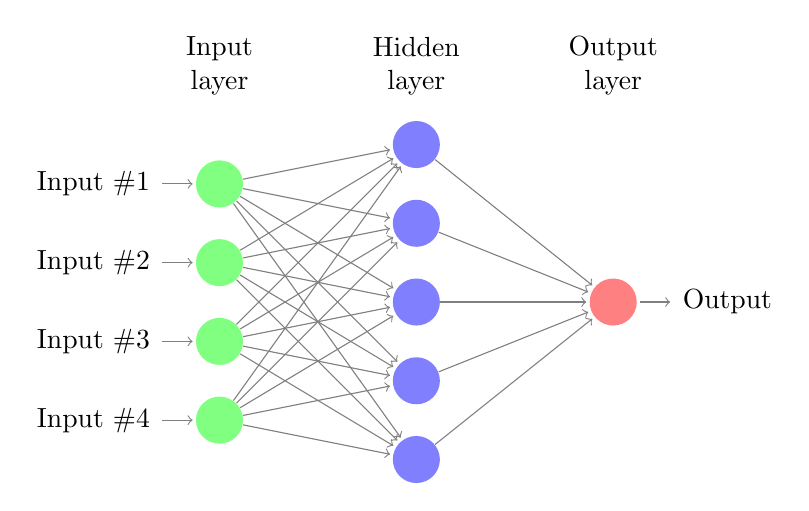
\begin{tikzpicture}[shorten >=1pt,->,draw=black!50, node distance=\layersep]
		\def\layersep{2.5cm}
		
		\tikzstyle{every pin edge}=[<-,shorten <=1pt]
		\tikzstyle{neuron}=[circle,fill=black!25,minimum size=17pt,inner sep=0pt]
		\tikzstyle{input neuron}=[neuron, fill=green!50];
		\tikzstyle{output neuron}=[neuron, fill=red!50];
		\tikzstyle{hidden neuron}=[neuron, fill=blue!50];
		\tikzstyle{annot} = [text width=4em, text centered]
		
		% Draw the input layer nodes
		\foreach \name / \y in {1,...,4}
		% This is the same as writing \foreach \name / \y in {1/1,2/2,3/3,4/4}
		\node[input neuron, pin=left:Input \#\y] (I-\name) at (0,-\y) {};
		
		% Draw the hidden layer nodes
		\foreach \name / \y in {1,...,5}
		\path[yshift=0.5cm]
		node[hidden neuron] (H-\name) at (\layersep,-\y cm) {};
		
		% Draw the output layer node
		\node[output neuron,pin={[pin edge={->}]right:Output}, right of=H-3] (O) {};
		
		% Connect every node in the input layer with every node in the
		% hidden layer.
		\foreach \source in {1,...,4}
		\foreach \dest in {1,...,5}
		\path (I-\source) edge (H-\dest);
		
		% Connect every node in the hidden layer with the output layer
		\foreach \source in {1,...,5}
		\path (H-\source) edge (O);
		
		% Annotate the layers
		\node[annot,above of=H-1, node distance=1cm] (hl) {Hidden layer};
		\node[annot,left of=hl] {Input layer};
		\node[annot,right of=hl] {Output layer};
	\end{tikzpicture}
	\caption{A common graphical representation of a neural network.}
	\label{figure:gr rep nn}
\end{figure}

A neural network is commonly graphically represented as seen in
figure \ref{figure:gr rep nn}. The reason the family
of functions are called neural networks is that
the graph resembles a biological neural network.\medskip

In practice a neural network is an alternating sequence between 
affine layers of the form $ f(x;A,b)=Ax+b $ for a weight 
$ (A,b)\in\RR^{m\times n}\times \RR^m $
and some choice of non-linear layers $ h:\RR^n\rightarrow\RR^m $,
such as the sigmoid function 
$ s:\RR\ra \RR;\,x\mapsto (1+\exp(-x))^{-1} $ or
the rectified linear unit function
$ \mathrm{ReLu}:\RR\ra \RR;\,x\mapsto\max\{0,x\} $
applied entry-wise to the input. These non-linear mappings
are called activation functions.\medskip

The approximation of the ideal function with some neural network
is prone to generalization errors. To combat this, we often add
a regularization function $ R:\RR^n\times \RR^m\ra \RR $. 
As an example we may demand that the 
output data to be sparse. In this case we could choose
$ R(x,\theta)=\abs{x_1}+\ldots+\abs{x_n} $ for 
$ (x,\theta)\in\RR^{n}\times\RR^m $. Our minimization
problem thus becomes 
\begin{align*}\label{equation:reg emp Bayes Risk}
	\minimize_{\theta\in \RR^k}
	\qquad &\qquad
	\int_{\rX\times \rY} L(f(x;\theta),y)+R(f(x;\theta),\theta)\,d\emMe(x,y).
	\tag{Reg-eBR}
\end{align*}

We extract two function definitions 
\begin{align*}
	\vp(\theta):=\int_{\rX\times \rY} L(f(x;\theta),y)\,d\emMe(x,y)
	\quad\text{ and }\quad
	\psi(\theta):=\int_{\rX\times \rY} R(f(x;\theta),\theta)\,d\emMe(x,y).
\end{align*}

and restate state our minimization problem as the general problem
\begin{align*}
	\minimize_{\theta\in \RR^k}
	\qquad &\qquad
	\vp(\theta)+\psi(\theta).
\end{align*}

Usually the only assumption we place on $ \vp $ is that
it is Lipschitz continuous. However for many applications 
we may assume that $ \vp $ is a proper convex
differentiable function and that $ \psi $ is a proper convex function
(cf. \cite[Section 3.1]{signoretto2014learning}).
In this case we know from 
% TODO find source
\cite{rockafellar2015convex} 
that $ \theta^{\ast}\in\RR^k $
is an optimal solution to the minimization problem
if and only if
\begin{align*}
	0\in \prt f(\theta^{\ast})+\prt g(\theta^{\ast}).
\end{align*} 
Provided that both $ \vp $ and $ \psi $ are l.s.c,
the operator $ A:=\prt f+\prt g $
is maximally monotone by 
corollary \ref{corollary:sub diff of pr lsc func is max mon op}.
We find the optimal solution by solving the evolution
equation \ref{equation:hom GSD}
with operator $ A $ and any
initial value $ \theta_0\in \RR^k $. In particular
we solve
\begin{align*}
	\begin{cases}
		\partial_t \theta+A\theta \ni 0 & \text{ on }[0,\plus\infty),\\
		\theta=\theta_0 & \text{ on }\{0\}.
	\end{cases}
\end{align*}

In practice it is far more efficient and suffices to approximate the solution
by the discrete gradient descent algorithm,
instead of solving the actual evolution
equation. The generalized discrete gradient
descent method is given by the forward Euler method  
\begin{align}\label{equation:disc grad desc meth}
	\begin{cases}
		\theta_t-(\idm_{\RR^k}-\alpha A)\theta_{t-1} \ni 0 & \text{ on }\NN,\\
		\theta_t=\theta_0 & \text{ on }\{0\}.
	\end{cases}
	\tag{gDGM}
\end{align}
for some user defined step size $ \alpha>0 $.
The theory of gradient flows applies
to non-convex functions as-well, however
fewer properties are known and the
asymptotic limit may change depending
on the initial value.

\subsection{Example Ridge Regression}
The paper \cite[Section 3.2]{signoretto2014learning} from M. Signoretto et al
mentions two examples of how the gradient descent method
can be applied, where the minimization function
is convex. Namely Ridge Regression \cite{hoerl1970ridge}
and Group Lasso \cite{jacob2009group}. We will present
an example of Ridge Regression as it is very simple,
a smooth and convex problem,
and it highlights important aspects of machine learning.
\smallskip

Ridge Regression is a method for solving the standard model for 
linear regression. Suppose that there
exists some unknown affine linear transformation
$ h:\RR^k\ra \RR $. We are given a finite dataset
$ (X_1,Y_1),\ldots,(X_n,Y_n)\in\RR^{k}\times \RR $
such that $ Y_i=h(X_i)+\varepsilon_i $ for
all $ 1\leq i\leq n $, where the variables
$ \varepsilon_1,\ldots,\varepsilon_n $
are unknown and are chosen i.i.d from some  
probability distribution.\smallskip

Naturally we will try to approximate the
linear functional $ h $ with a single
layer affine neural network defined by
$ f(x;a,b):=a^t x+b $ for any 
$ x,a\in\RR^k $ and $ b\in\RR $.\smallskip

We define our loss function $ L $ as the squared error 
\begin{align*}
	L(x,y):=\frac{1}{2}(x-y)^2
	\qquad\forall x,y\in\RR.
\end{align*}

We want to control the growth of
the weights $ a,b $ with some
user defined
parameter $ \lambda>0 $ by the 
regularization function
\begin{align*}
	R(a,b):=\frac{\lambda}{2}(a^ta+b^2)
	\qquad\forall (a,b)\in\RR^k\times\RR.
\end{align*}

Our problem statement \ref{equation:reg emp Bayes Risk}
thus becomes
\begin{align*}
	\minimize_{(a,b)\in \RR^n\times\RR}
	\qquad &\qquad
	\frac{\lambda}{2}(a^ta+b^2)+
	\frac{1}{2n}\sum_{i=1}^n (Y_i-f(X_i;a,b))^2.
\end{align*}

We use matrix notation to simplify the above expression.
To that end define $ X\in\RR^{n\times k} $ by $ X:=(X_1,\ldots, X_n)^t $,
define $ Y\in\RR^n $ by $ Y:=(Y_1,\ldots,Y_n) $ and define
the vector the constant one vector $ e:=(1,\ldots,1)\in\RR^n $. We compute
\begin{align*}
	\frac{1}{2n}\sum_{i=1}^n (Y_i-f(X_i;a,b))^2
	&=\frac{1}{2n}(Y-Xa-be)^t(Y-Xa-be)\\
	&=\frac{1}{2n}
	\begin{pmatrix}
		a \\ b
	\end{pmatrix}^t
	\begin{pmatrix}
		X^t X & 0\\
		0 & 1
	\end{pmatrix}
	\begin{pmatrix}
		a \\ b
	\end{pmatrix}
	-\frac{1}{n}
		Y^t 
	\begin{pmatrix}
		X & e
	\end{pmatrix}
	\begin{pmatrix}
		a \\ b
	\end{pmatrix}
	+\frac{1}{2n}Y^tY.
\end{align*}
Then the \ref{equation:reg emp Bayes Risk} equation can be simplified to

\begin{align*}
	\minimize_{(a,b)\in \RR^n\times\RR}
	\quad &\quad
	\begin{pmatrix}
		a \\ b
	\end{pmatrix}^t
	\left(
	\frac{\lambda}{2}
	\idm_{\RR^{k+1}}
	+
	\frac{1}{2n}
	\begin{pmatrix}
		X^t X & 0\\
		0 & 1
	\end{pmatrix}
	\right)
	\begin{pmatrix}
		a \\ b
	\end{pmatrix}
	-\frac{1}{n}
		Y^t
	\begin{pmatrix}
		X & e
	\end{pmatrix}
	\begin{pmatrix}
		a \\ b
	\end{pmatrix}
	+\frac{1}{2n}Y^tY.
\end{align*}
We see that we must minimize a quadratic polynomial, which happens
to be a proper convex smooth problem. Thus our theory is applicable.\smallskip

To deduce the discrete gradient descent method
we must simply compute the derivative of $ a $
and $ b $
\begin{align*}
	\Delta(a,b):=&\prt_{(a,b)}
	\begin{pmatrix}
		a \\ b
	\end{pmatrix}^t
	\left(
	\frac{\lambda}{2}
	\idm_{\RR^{k+1}}
	+
	\frac{1}{2n}
	\begin{pmatrix}
		X^t X & 0\\
		0 & 1
	\end{pmatrix}
	\right)
	\begin{pmatrix}
		a \\ b
	\end{pmatrix}
	-\frac{1}{n}
		Y^t
	\begin{pmatrix}
		X & e
	\end{pmatrix}
	\begin{pmatrix}
		a \\ b
	\end{pmatrix}
	+\frac{1}{2n}Y^tY\\
	&\qquad=\left(
	\lambda\idm_{\RR^{k+1}}
	+
	\frac{1}{n}
	\begin{pmatrix}
		X^t X & 0\\
		0 & 1
	\end{pmatrix}
	\right)
	\begin{pmatrix}
		a \\ b
	\end{pmatrix}
	-\frac{1}{n}
	\begin{pmatrix}
		X^t \\ e^t
	\end{pmatrix}
	Y.
\end{align*}

The discrete gradient descent method is therefore given by
\begin{align*}
	\begin{cases}
		(a_t,b_t)-(a_{t-1},b_{t-1})
		+\alpha \Delta(a_{t-1},b_{t-1}) = 0 & \text{ on }\NN,\\
		(a_t,b_t)=(a_0,b_0) & \text{ on }\{0\}.
	\end{cases}
\end{align*}

\subsubsection{Numerical Experiment}
We end the paper by presenting a concrete example of ridge
regression\footnote{all of the code that
was used in this experimenter is found in the following
GitHub repository}. Given some dimension $ k $, some fixed $ a_{\mathrm{real}}\in\RR^k $
and $ b_{\mathrm{real}}\in\RR $, we will use the discrete gradient descent method to
approximate the linear functional
$ h_{\mathrm{real}}(x):=a_{\mathrm{real}}^t x +b_{\mathrm{real}}$.
We choose $ n $ points $ X_1,\ldots,X_n $ independently under
a uniform distribution from an open subset $ \Omega\subseteq\RR^k $.
For some user defined $ \sigma>0 $, we draw $ n $
values $ \varepsilon_1,\ldots,\varepsilon_n $ independently 
from the normal distribution
$ \mathcal{N}(0,\sigma^2) $ and define $ Y_i:=h_{\mathrm{real}}(X_i)+\varepsilon_i $
for $ 1\leq i\leq n $. We choose the initial weights $ (a_0,b_0) $ uniformly
randomly from an open set $ \Theta\subseteq\RR^k\times\RR $.\medskip

This numerical experiment is conducted using MatLab
and the standard random number generator provided by MatLab.
The source code is available at this public
\href{https://github.com/JethroWarnettMath/Semester-Project-Gradient-Flow-HS2021}
{GitHub} repository.\medskip

For our experiment we set $ k=2 $, 
$a_{\mathrm{real}}=(1,-1)$, $ b_{\mathrm{real}}=2 $,
$ \Omega=[-10,10]^2 $ and $ \Theta=[-10,10]^3 $. 
With these parameters we let the discrete gradient descent
algorithm run for a $ 1000 $ iterations. We repeat the
experiment $ 10 $ times and plot the results in the
following figures:\smallskip 

In figure 3 %\ref{fig:exampleA} 
we show how the parameter $ a_t $ evolves depending
on its initial weight. We
see that for each starting value the graphs 
more or less converge in a straight line to 
the value $ a_{\mathrm{real}} $. \smallskip

In figure 4 we
present how the parameter $ b_t $ changes depending
on its initial weight. Again we
see that for each starting value the graphs 
converge to the value $ b_{\mathrm{real}} $. \smallskip

Finally in figure 5 we
present how the parameter $ a_b $ develops depending
on its initial weight. For each starting value the graphs 
decay linearly to $ 0 $.

\begin{figure}[H]
	\centering
	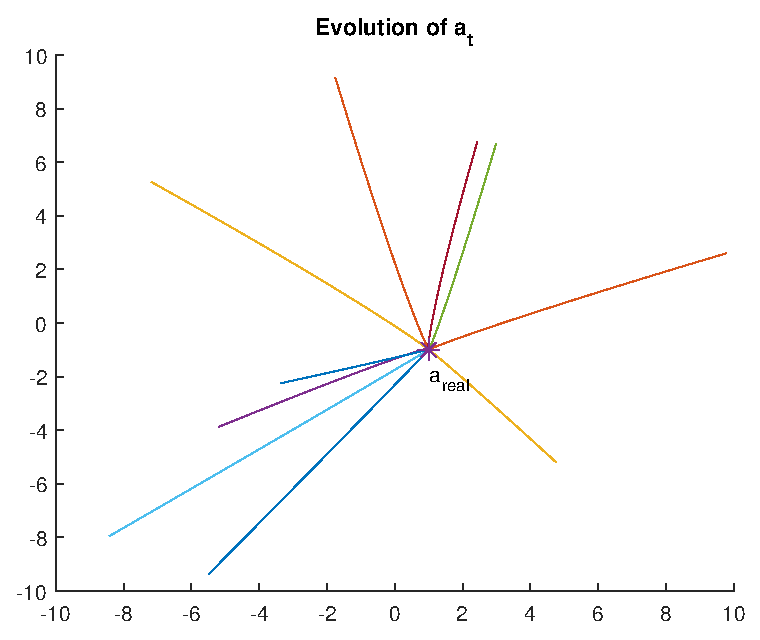
\includegraphics[width=0.5\linewidth]{EvolutionA}
	\caption{The evolution of $ a_t $ in the
	discrete gradient descent method for different
	initial values.}\label{fig:exampleA}
\end{figure}

\begin{figure}[H]
	\centering
	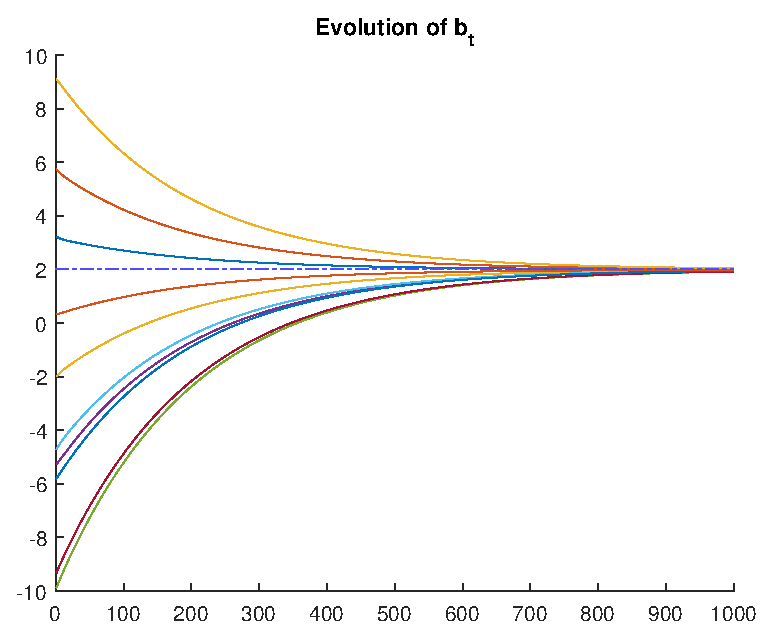
\includegraphics[width=0.5\linewidth]{EvolutionB}
	\caption{The evolution of $ b_t $ in the
		discrete gradient descent method for different
		initial values.}\label{fig:exampleB}
\end{figure}

\begin{figure}[H]
	\centering
	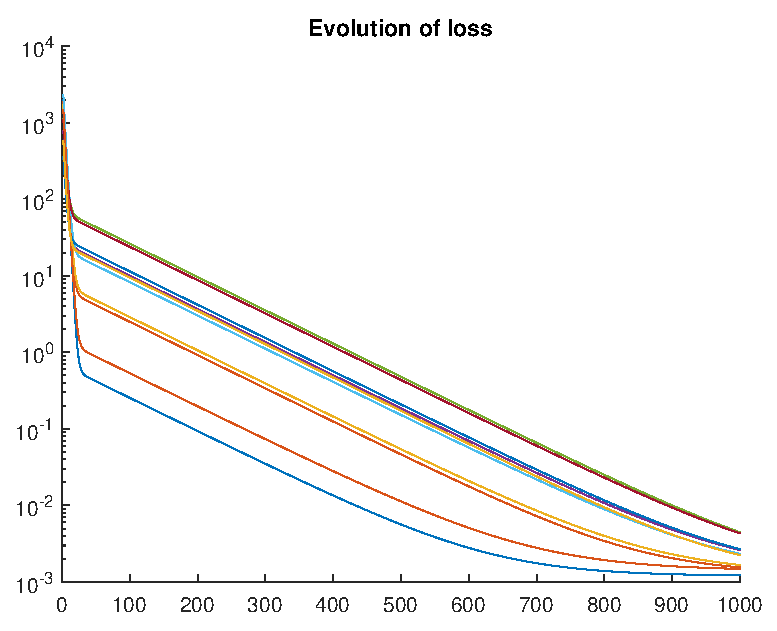
\includegraphics[width=0.5\linewidth]{EvolutionLoss}
	\caption{The evolution of the loss function in the
		discrete gradient descent method for different
		initial values. Note that the scale is logarithmic
		in the y axis.}\label{fig:exampleLoss}
\end{figure}
	\endgroup
	
	\bibliographystyle{plain}
	\bibliography{ref.bib} 
	
\end{document}